\chapter{Unfolding}\label{chap:conclusion}
  To correct for detector and imperfect reconstruction effects in a measurement, we often unfold, or transform the detector level distribution to the particle level; we can see these effects even in one dimension by comparing the reconstructed and generated distributions for the same events \ref{fig:genreco}. Unfolding is performed by creating an $n\times m$ response matrix, $\mathbf{M}$, from simulation, where axis $m$ corresponds to the particle level distibution and axis $n$ the detector level distribution. Naiveley, one would expect to be able to correct the detector level distribution to the particle level distribution by setting up the following equation,
  \begin{equation}
    \label{eq:unfold1}
    y_i = \Sigma_{i=1}^{m}A_{ij}x_j, \, 1 \leq i \leq n
  \end{equation}
  where $y_i$ represents the detector level distribution, or observed event counts, $A_{ij}$ is the probability matrix that describes the migration from a bin $j$ at the particle level to any bin at the detector level, and $x_j$ the true or particle level distribution, and solve for $x_j$ by inverting the probability matrix, $A_{ij}$. However, any statistical fluctuations in $y_i$ are amplified by this rudimentary method. We instead use the TUnfold algorithm \cite{tunfold} which employs a least squares approach to estimate the true distribution $\tilde{x_j}$.
  \begin{figure}[h!]
    \centering
    	\begin{subfigure}
		\centering
		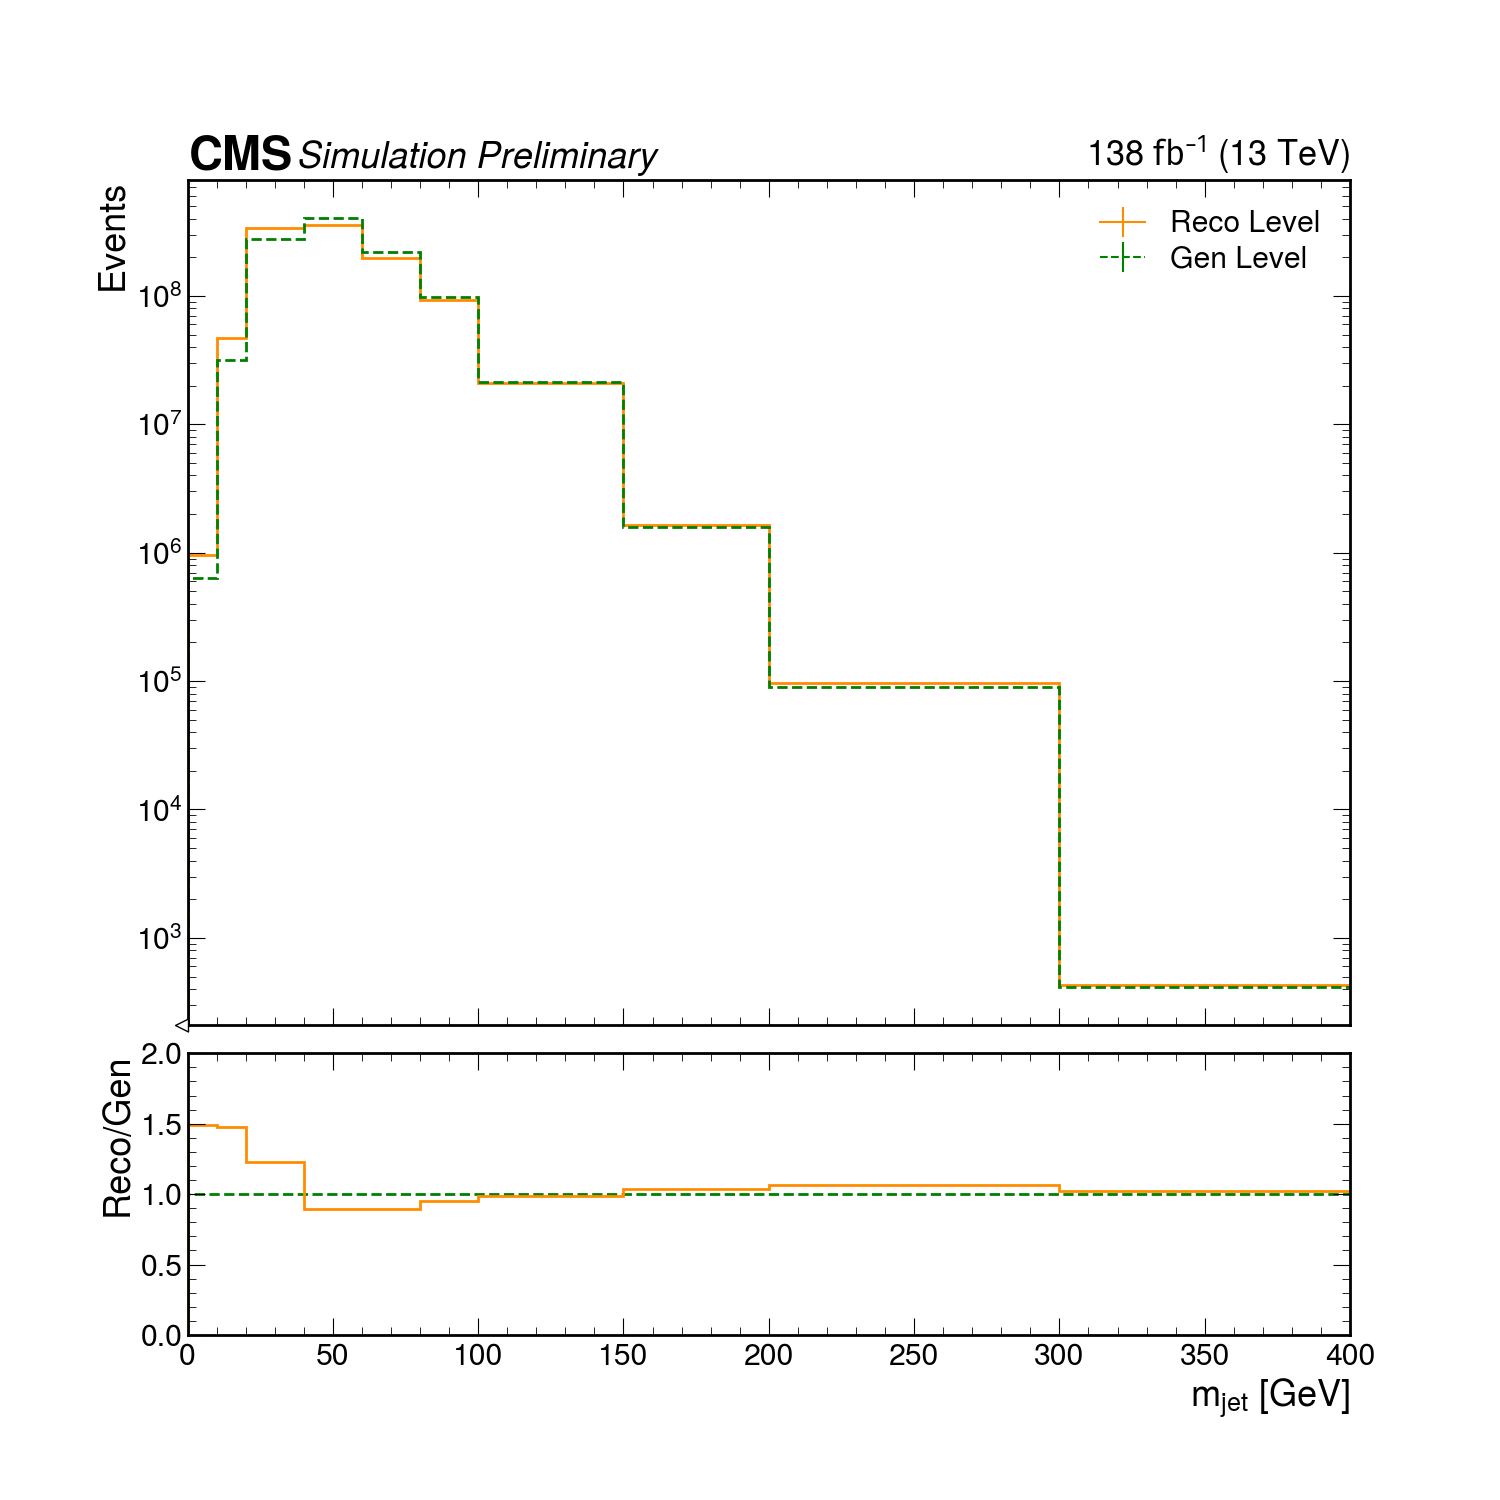
\includegraphics[width=0.45\textwidth]{figures/multijet/dijet/genreco_mjet.png}
              \end{subfigure}%
         \begin{subfigure}
		\centering
		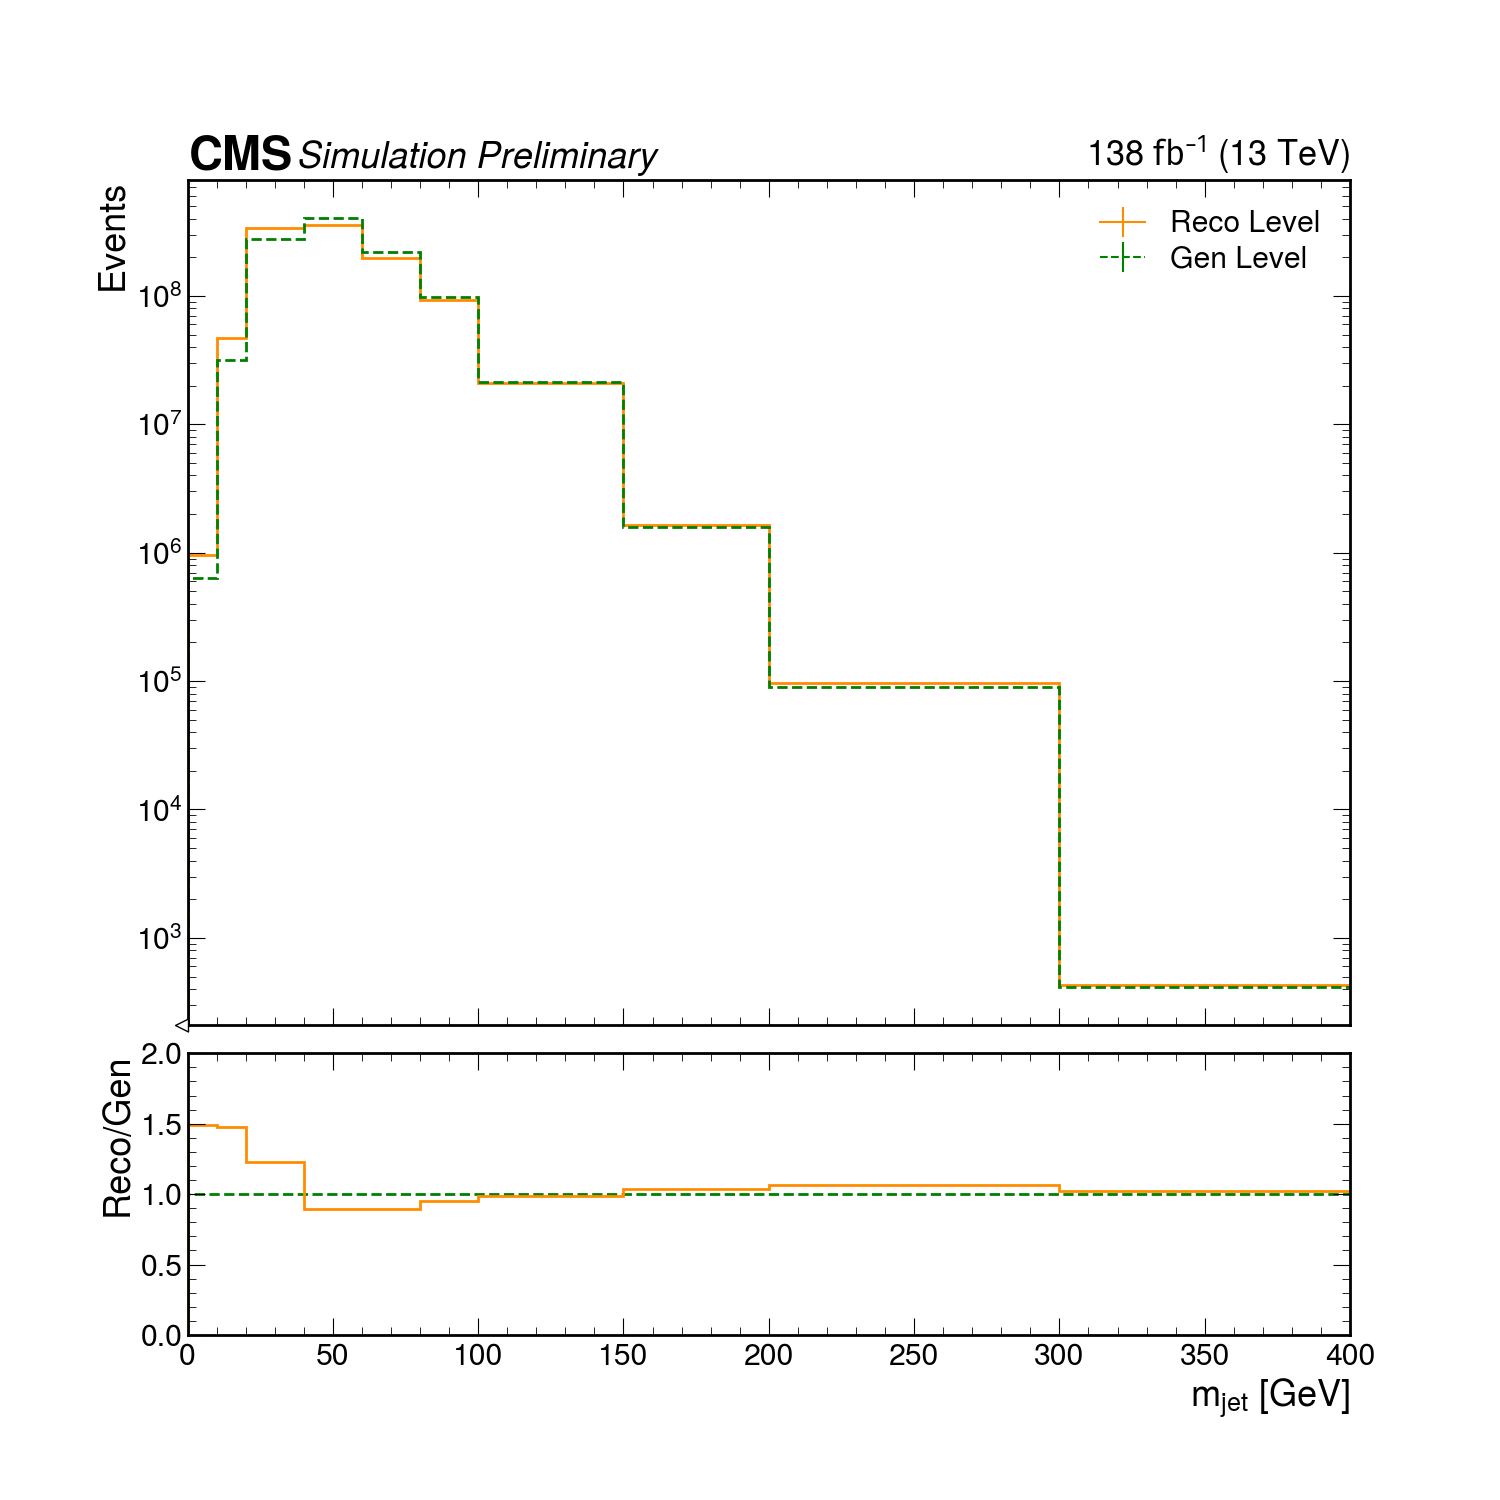
\includegraphics[width=0.45\textwidth]{figures/multijet/dijet/genreco_mjet.png}
	\end{subfigure}%
    \caption{Distributions of the generated (orange) and reconstructed (green) ungroomed mass distributions. The left is the dijet distribution and the right is the trijet.}
    \label{fig:genreco}
  \end{figure}
  \section{The TUnfold algorithm}
   The TUnfold algorithm, interfaced through ROOT \cite{root}, finds the true distribution while avoiding the inversion problem by finding $\mathbf{x}$ that minimizes the Lagrangian, $\mathcal{L}(x,\lambda)$.
 \begin{equation}
   \mathcal{L}(x, \lambda) = \mathcal{L}_1 + \mathcal{L}_2 + \mathcal{L}_3
 \end{equation}
  \begin{equation}
   \mathcal{L}_1 = (\mathbf{y}-\mathbf{A}\mathbf{x})^{\intercal}\mathbf{V_{yy}}^{-1} (\mathbf{y}-\mathbf{A}\mathbf{x})
 \end{equation}
  \begin{equation}
 \mathcal{L}_2 = \tau^2(\mathbf{x}-f_b\mathbf{x_0})^{\intercal}(\mathbf{L^{\intercal}L})(\mathbf{x}-f_b\mathbf{x_0})
 \end{equation}
  \begin{equation}
   \mathcal{L}_3 = \lambda(Y-\mathbf{e^{\intercal}x})
 \end{equation}
   \begin{equation}
     Y = \sum_iy_i
   \end{equation}
      \begin{equation}
     e_j = \sum_iA_{ij}
   \end{equation}
   $\mathcal{L}_1$ gives the output of the least squares minimisation without any additional regularisation or area constraint. The vector $\mathbf{y}$ is the data distribution of dimension n, $\mathbf{A}$ is the probability matrix; it describes the probability of bin row $j$ of $\mathbf{x}$ migrating to to bin $i$ of $\mathbf{y}$ and is an $n \cross m $ matrix. $\mathbf{x}$ is our unfolding result once this equation is minimised and is of length $m$. $\mathbf{V_{yy}}$ is the covariance matrix of $\mathbf{y}$ and holds the square of the statistical uncertainties of the data. \\
   $\mathcal{L}_2$ describes the regularisation, which damps the fluctuations in $\mathbf{x}$. These fluctuations originate from the statistical fluctuations on $\mathbf{y}$ that are amplified in the minimizing $\mathcal{L}(x, \lambda)$.$\tau$ is the regularisation strength. The bias vector $f_b\mathbf{x_o}$ is composed of a normalization factor $f_b$ and a vector $\mathcal{x_0}$, which is the true distribution from simulation. The matrix $\mathbf{L}$ encodes the dimensions of the regularisation. In the simplest case of regularising a one dimensional distribution with no bias ($f_b=0$), this is an $n\cross n$ unity matrix, but in any other case this is an $n_R \cross n$ matrix, with $n_R$ being the number of regularisation conditions. \\
   $\mathcal{L}_3$ describes the area constraint. If the area constraint is enforced, the result $\mathbf{x}$ is required to match the total event count of $\mathbf{y}$, $Y$, after normalisation and correction of the efficiency vector, $\mathbf{e}$. This procedure limits prossible biases on the normalisation present if the data, $\mathbf{y}$, followes Poission's statistics instead of a normaldistribution that the least squares ansatz is valid for. $\lambda$ is a free parameter; if it is set to zero, the stationary point of $\mathcal{L}$ is found by setting just the derivatives of $\mathcal{L}_1+\mathcal{L}_2$ with respect to $\mathbf{x}$ equal to zero.\\
   Since we are currently not using regularisation, the lagrangian simplifies to $\mathcal{L}(x, \lambda) = \mathcal{L}_1(x)$ and the stable point is found by simply taking the derivative of this equation w.r.t $\mathbf{x}$ and setting it equal to zero.\\
   \subsubsection{Normalisation of the probability matrix and treatment of misses}
   In most cases, the probability matrix $\mathbf{A}$ is determined from Monte Carlo simulation, and initialised as a response matrix $\mathbf{M}$ of event counts where $\mathbf{M}$ has $n+1$ rows and m columns, one more row than the $n\cross m$ probability matrix, $\mathbf{A}$. The extra row is used to count events htat are generated in a particular bin $j$, but not found in any of the reconstructed bins; i.e. misses. These are treated nin the ROOT TUnfold implementation as an underflow bin on the Reco axis in the two-dimensional histogram of migrations representing the response matrix.\\
   In the TUnfold algorithm, \mathbf{A} and \mathbf{x_0} are initialised from \mathbf{M} as
   \begin{equation}
     A_{ij} = \frac{M_{ij}}{s_j}
   \end{equation}
   \begin{equation}
     s_j = \sum_{i=0}^nM_{ij}
   \end{equation}
      \begin{equation}
\mathbf{x_0}_j=s_j
   \end{equation}
   In other words, the 'truth' vector $\mathbf{x_0}$ is taken as the projection along the generator axis of the response matrix, and the probability matrix is the response matrix divided by the truth vector. In this setup, all matrices and vectors begin from the index 1, and the misses are filled along $\mathbf{M_{0j}}$. \\
      We also consider any events which could be reconstructed in the bins of $\mathbf{y}$, but do not originate from any of the signal bins of $\mathbf{x}$ as a background that should be subtracted prior to unfolding. This includes any background physics properties, but also includes events that are reconstructed in the detector in simulation, but have no corresponding generated object; i.e. fakes. This background subtraction is implemented in TUnfold as
   \begin{equation}
     \mathbf{y} = \mathbf{y_0}-f_b\mathbf{b}
   \end{equation}
   \begin{equation}
     (\mathbf{V_{yy}})_{ij} =  (\mathbf{V_{yy}})^0_{ij} + \delta_{ij}(f_b(\mathbf{\delta b}}_i)^2+(\delta f_b)^2b_ib_j
 \end{equation}
 Where $\mathbf{y_0}$ and $(\mathbf{V_{yy}})^0$ is initial the reconstructed distribution and the correspondonding covariance matrix before subtracting the backgrounds, $mathbf{b}$ is the background distribution, $\mathbf{\delta b}$ is the uncertainties on this distribution, and $f_b$ and $\delta f_b$ are the normalisation factor and its uncertainty. As can be seen in the above equation, the uncertainties on the background shape only contribute to the diagonals of the covariance matrix $\mathbf{V_{yy}}$. \\
  In the dijet and trijet channels, we do not have any significant physics backgrounds as we are measuring purely QCD processes, so the only thing we subtract before unfolding are the fakes. The fake rates can be seen in Figures \ref{fig:fakeratesbinned_dijet_u} and \ref{fig:fakeratesbinned_dijet_u} for the dijet channel and in Figures \ref{fig:fakeratesbinned_trijet_u} and \ref{fig:fakeratesbinned_trijet_g} for the trijet channel.
    \begin{figure}[htp!]
	\centering
	\begin{subfigure}
		\centering
		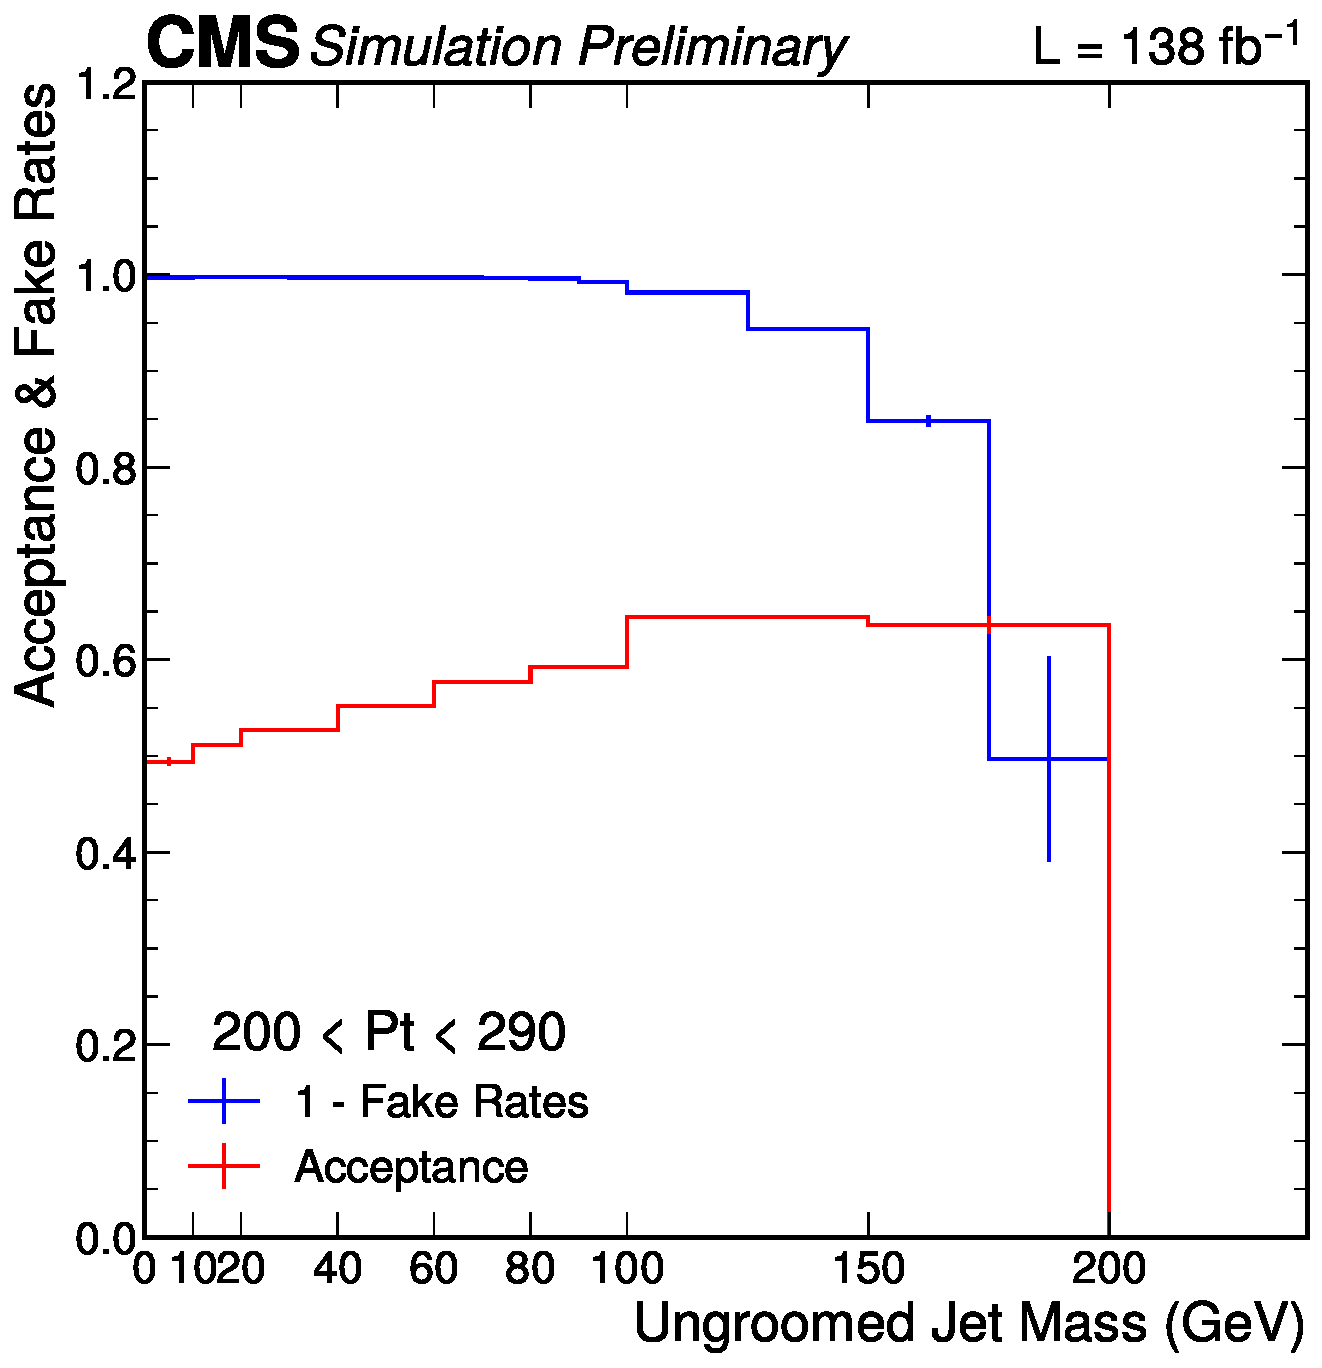
\includegraphics[width=0.45\textwidth]{figures/multijet/dijet/fakerates_ungroomed_0.pdf}
              \end{subfigure}%
                \begin{subfigure}
		\centering
		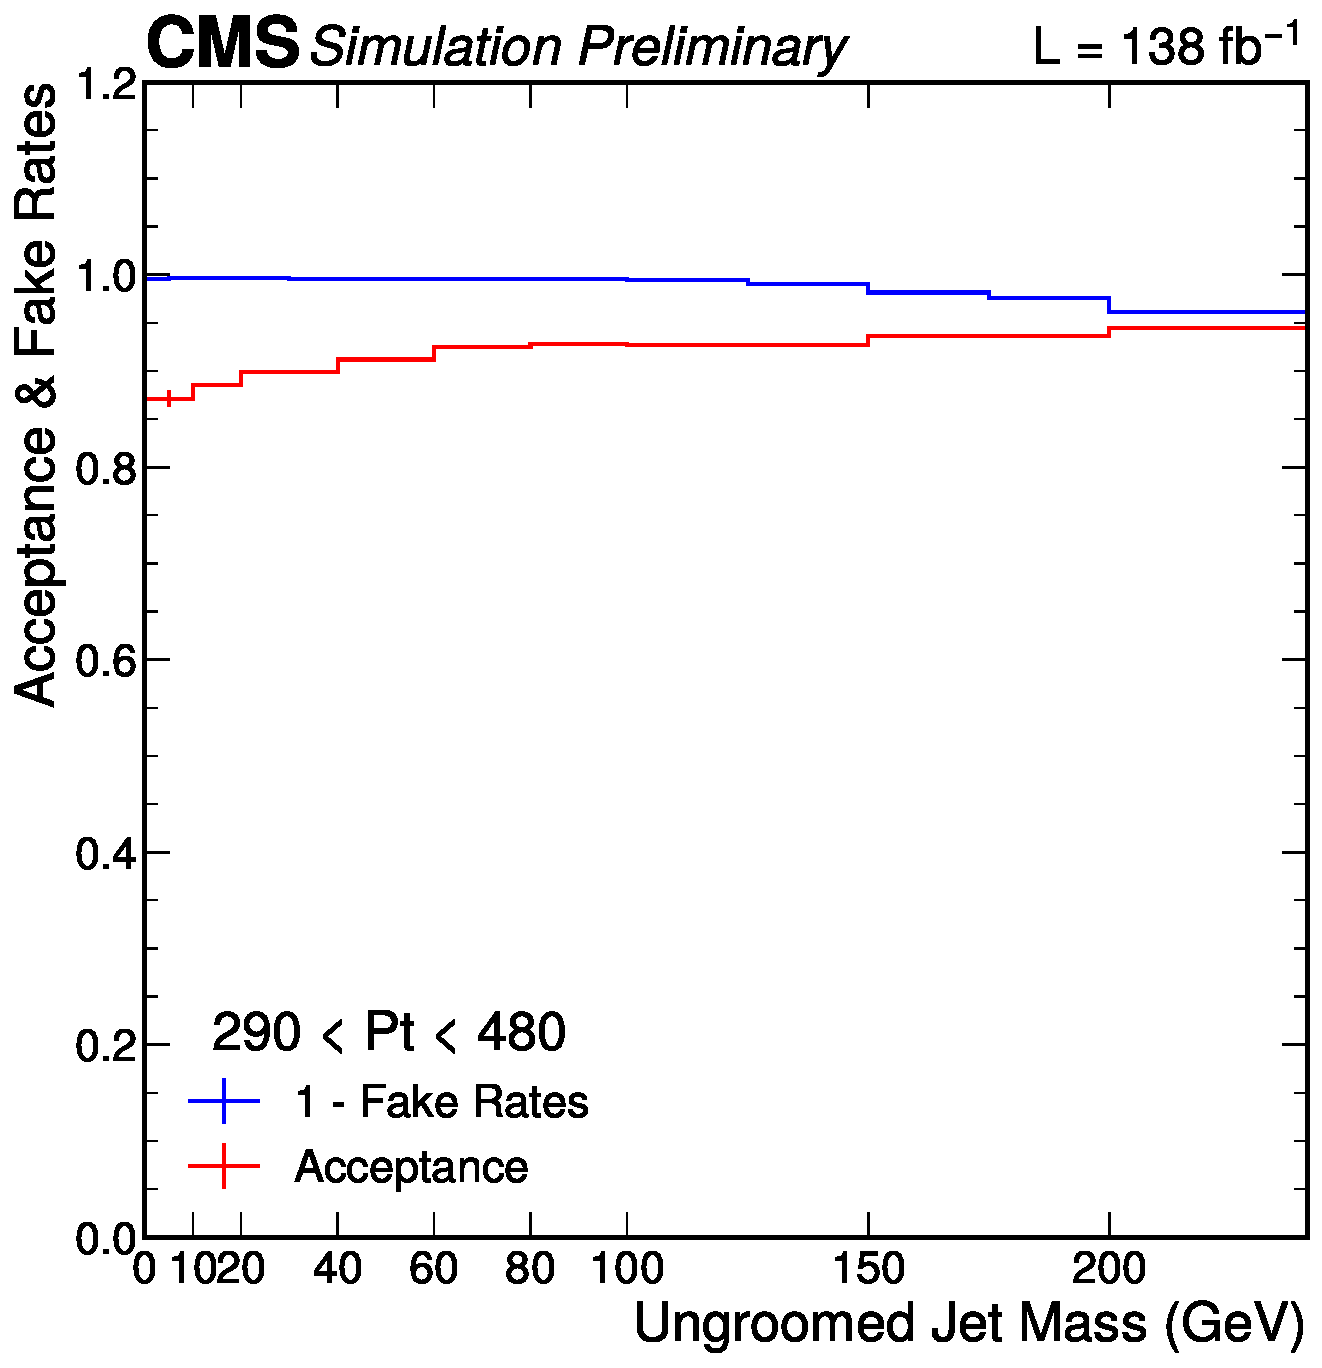
\includegraphics[width=0.45\textwidth]{figures/multijet/dijet/fakerates_ungroomed_1.pdf}
              \end{subfigure}\\
              \begin{subfigure}
		\centering
		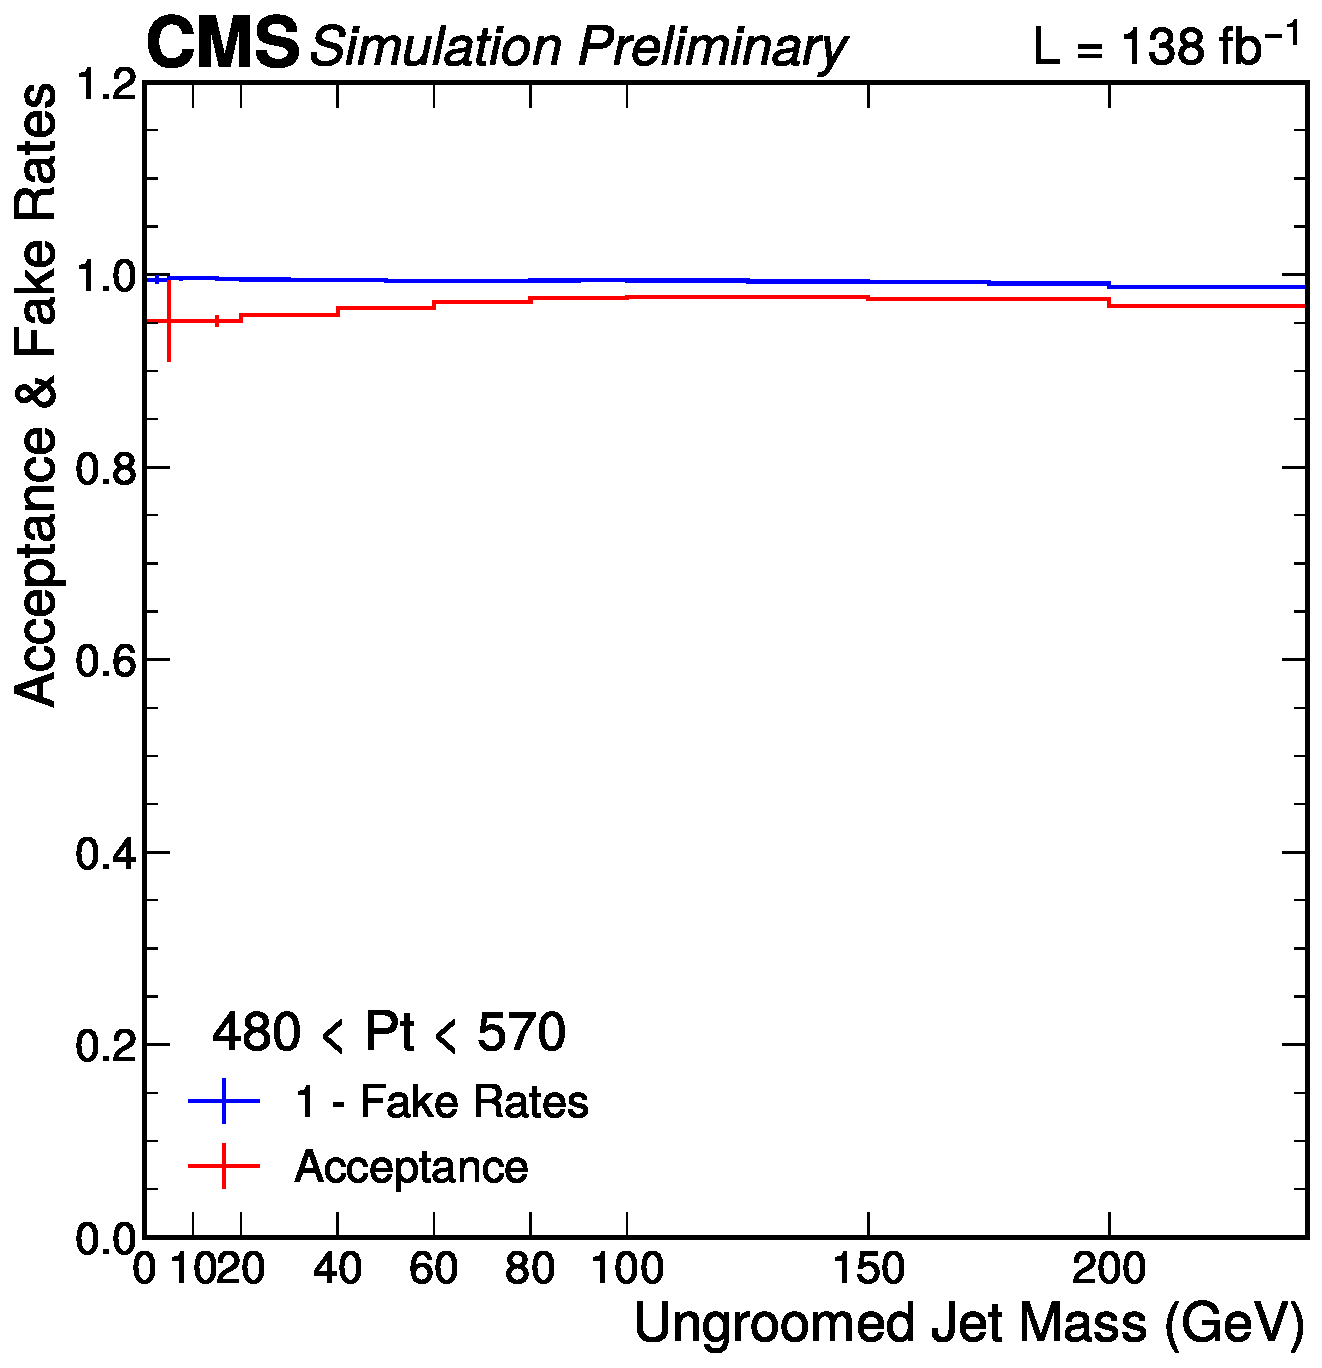
\includegraphics[width=0.45\textwidth]{figures/multijet/dijet/fakerates_ungroomed_2.pdf}
              \end{subfigure}
              \begin{subfigure}
		\centering
		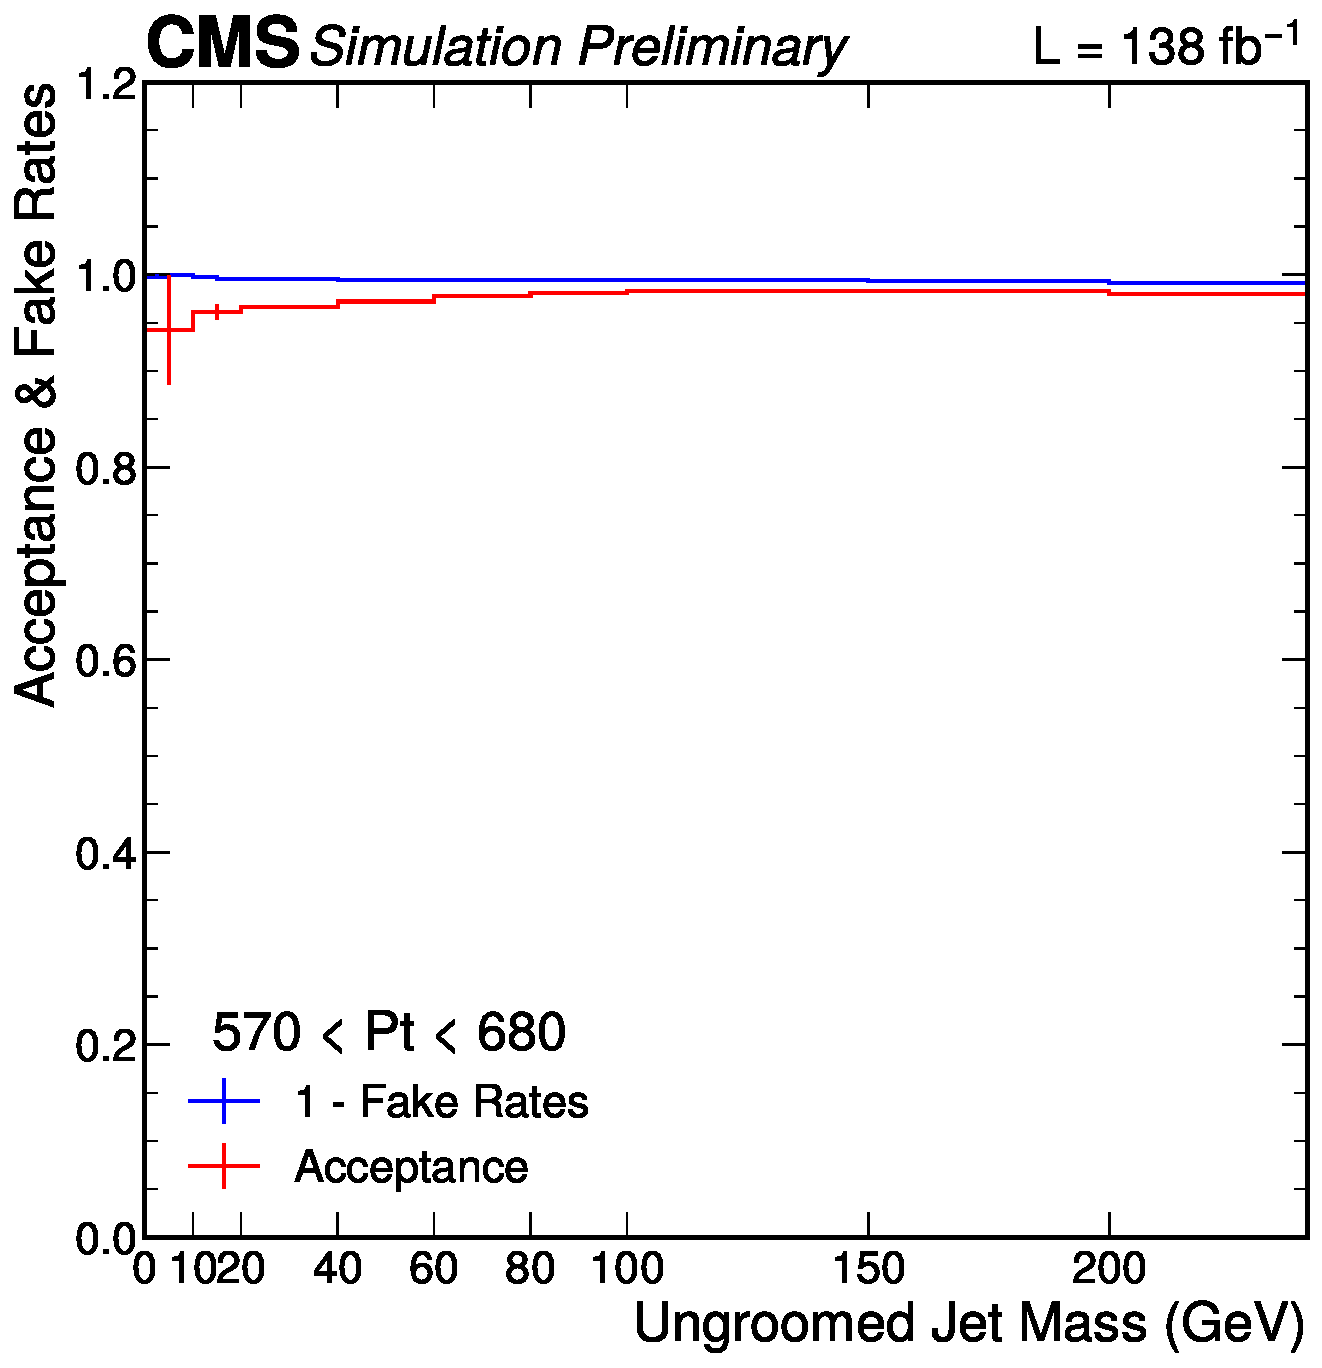
\includegraphics[width=0.45\textwidth]{figures/multijet/dijet/fakerates_ungroomed_3.pdf}
              \end{subfigure}\\
              \begin{subfigure}
		\centering
		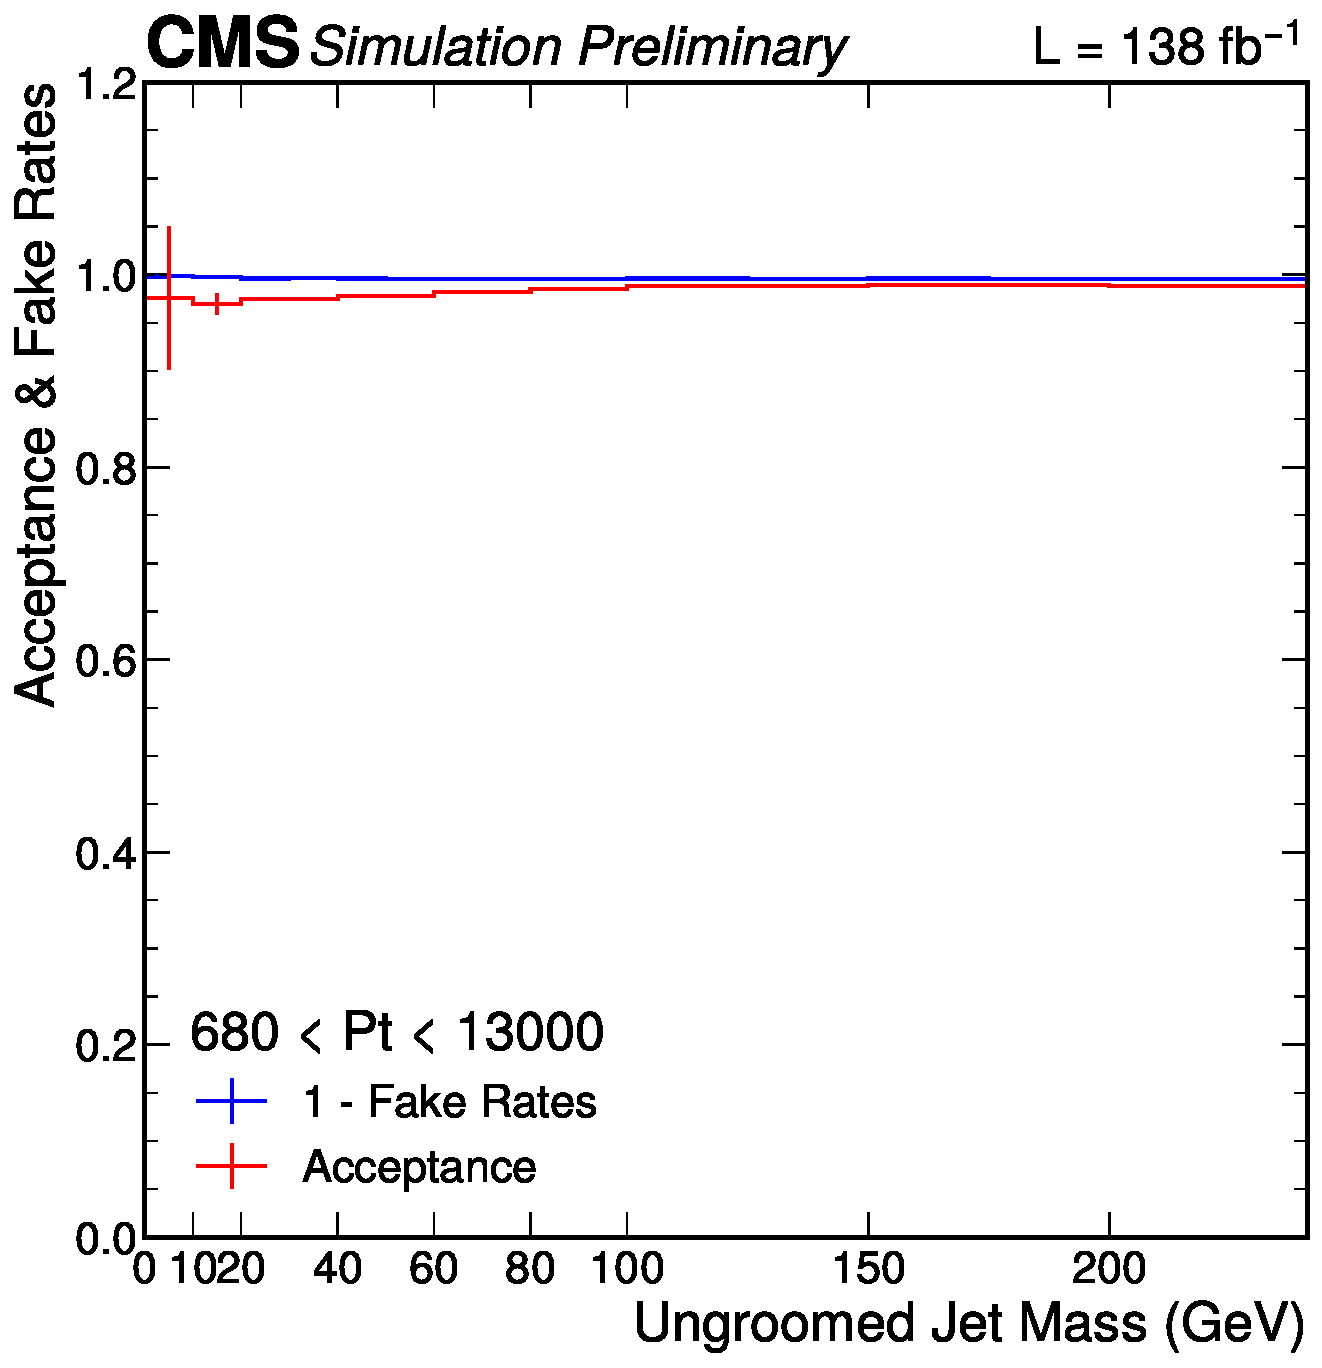
\includegraphics[width=0.45\textwidth]{figures/multijet/dijet/fakerates_ungroomed_4.pdf}
              \end{subfigure}
              	\caption{Fake and acceptance rates as a function of ungroomed jet mass for each pt bin for the dijet channel.}
	\label{fig:fakeratesbinned_dijet_u}
      \end{figure}
      
      \begin{figure}[htp!]
        \begin{subfigure}
          \centering
          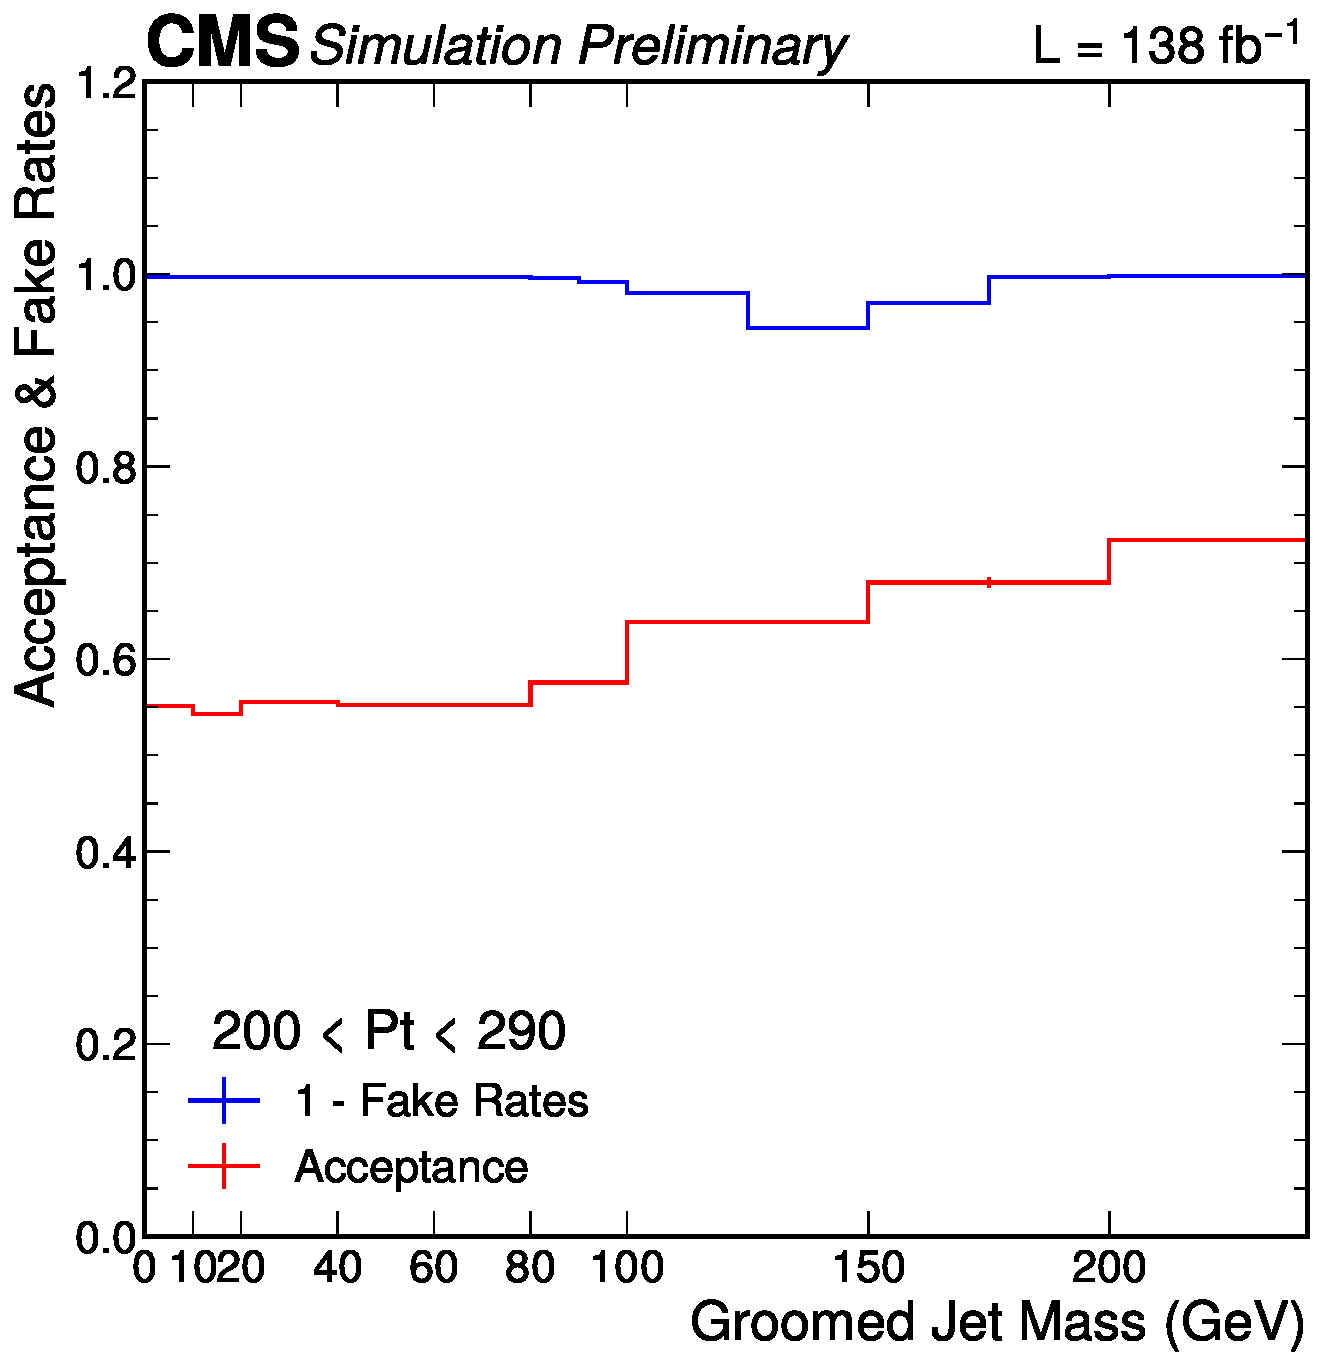
\includegraphics[width=0.45\textwidth]{figures/multijet/dijet/fakerates_groomed_0.pdf}
        \end{subfigure} 
        \begin{subfigure}
          \centering
          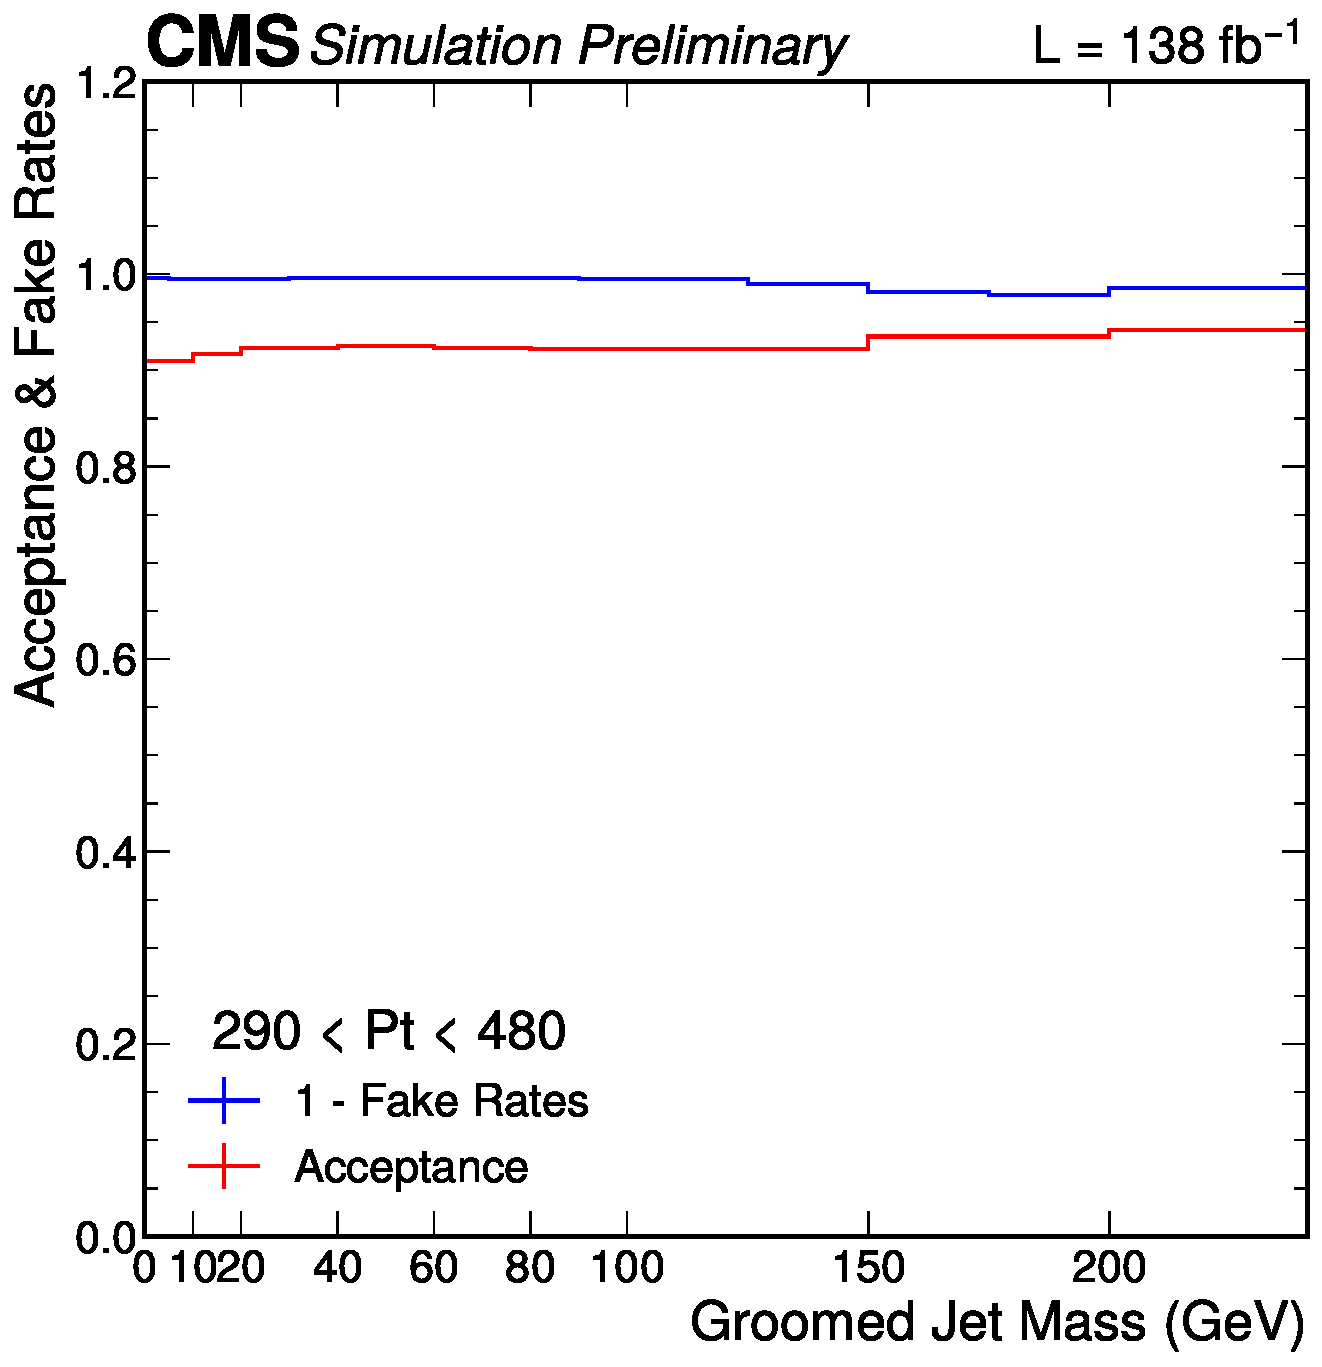
\includegraphics[width=0.45\textwidth]{figures/multijet/dijet/fakerates_groomed_1.pdf}
        \end{subfigure} \\
        \begin{subfigure}
          \centering
          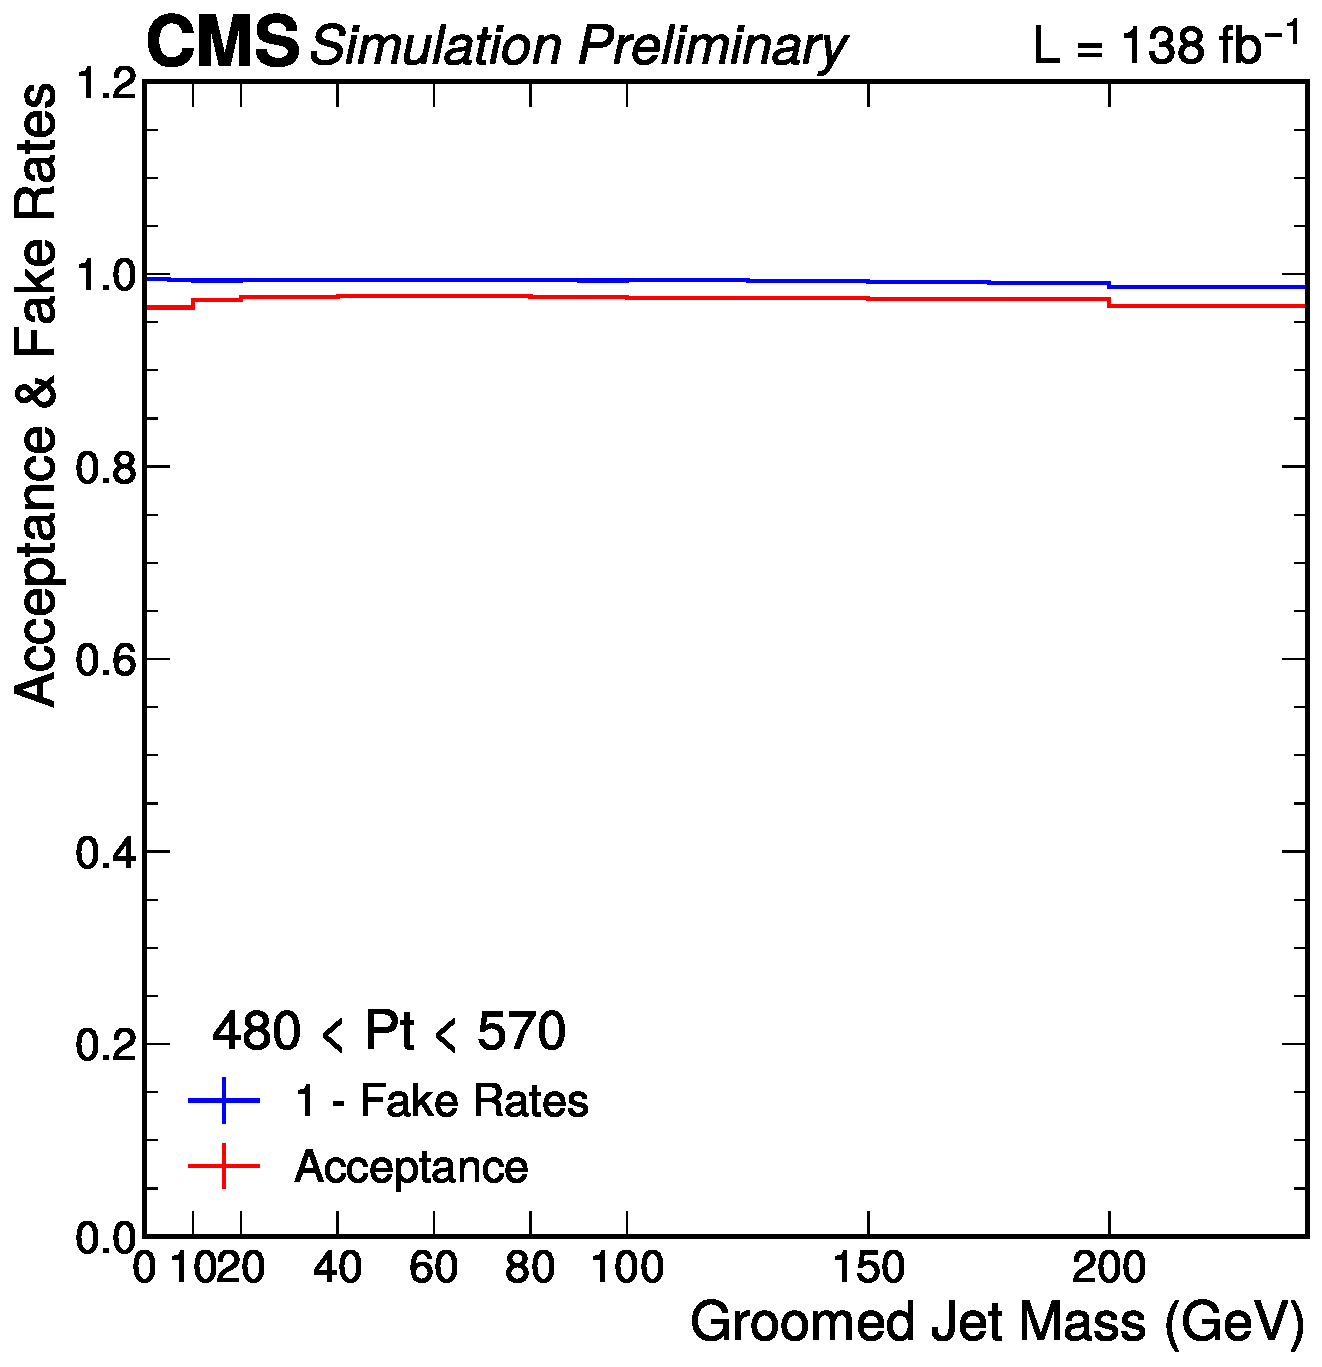
\includegraphics[width=0.45\textwidth]{figures/multijet/dijet/fakerates_groomed_2.pdf}
        \end{subfigure} 
        \begin{subfigure}
          \centering
          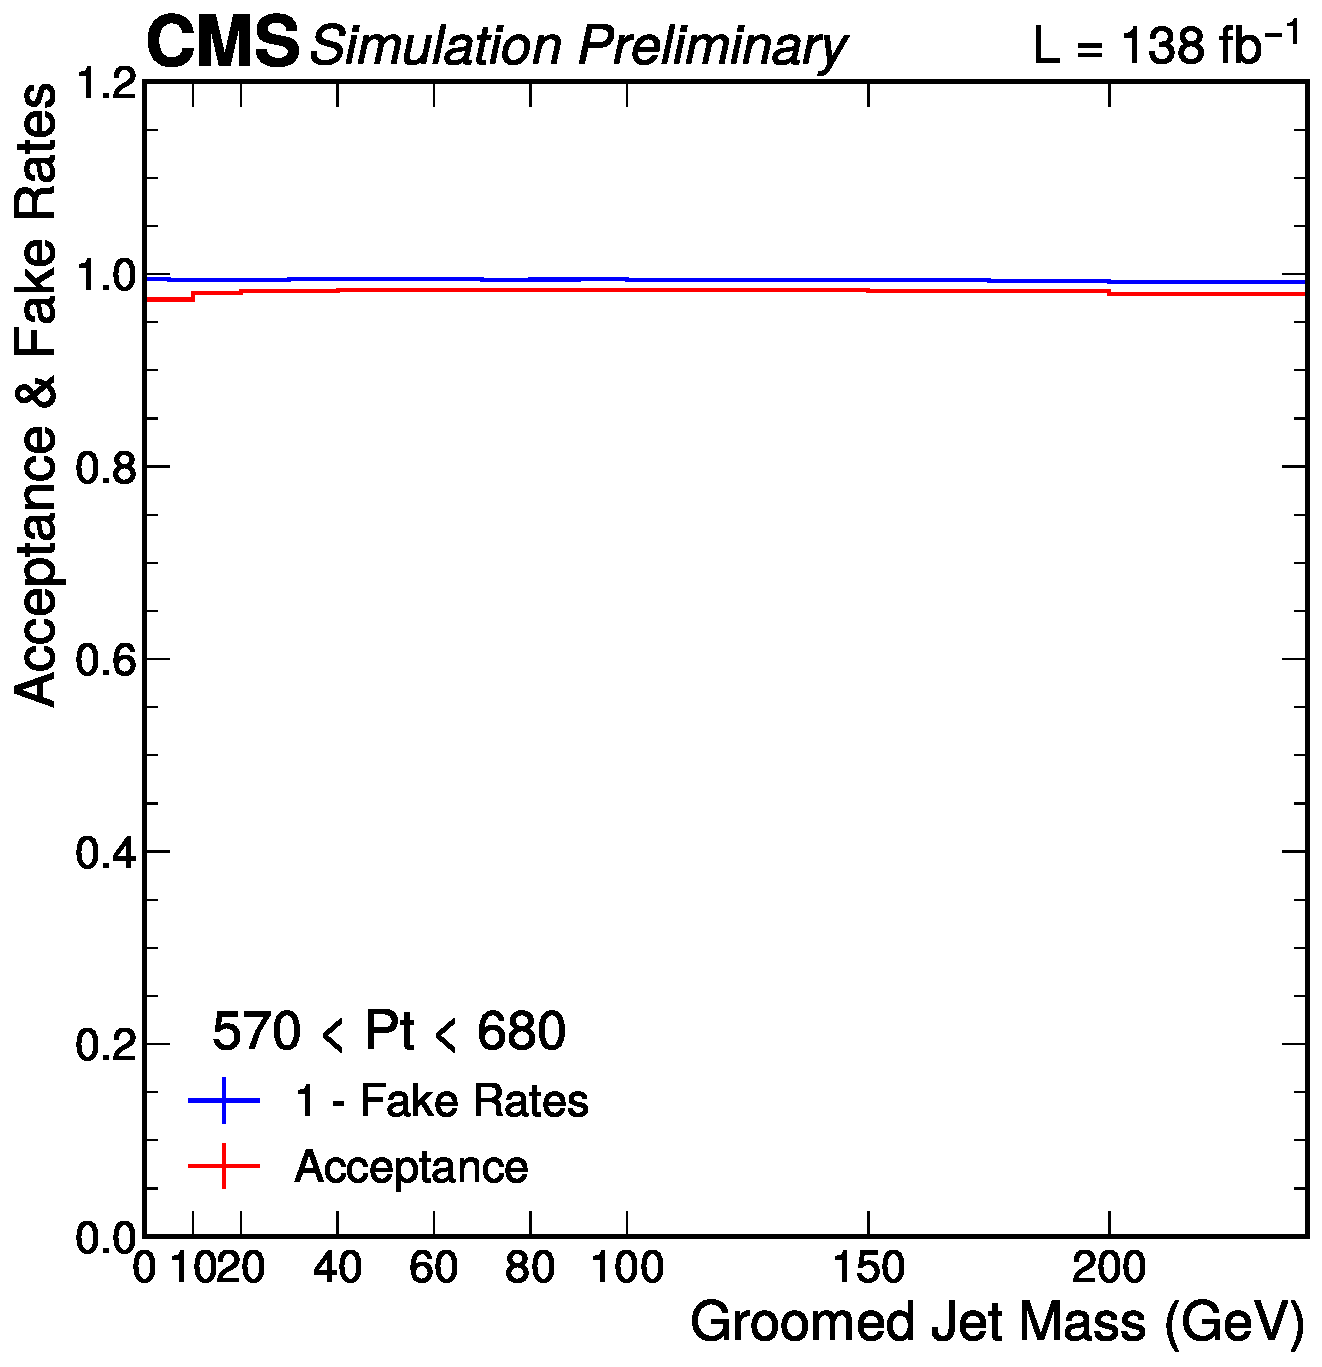
\includegraphics[width=0.45\textwidth]{figures/multijet/dijet/fakerates_groomed_3.pdf}
        \end{subfigure} \\
        \begin{subfigure}
          \centering
          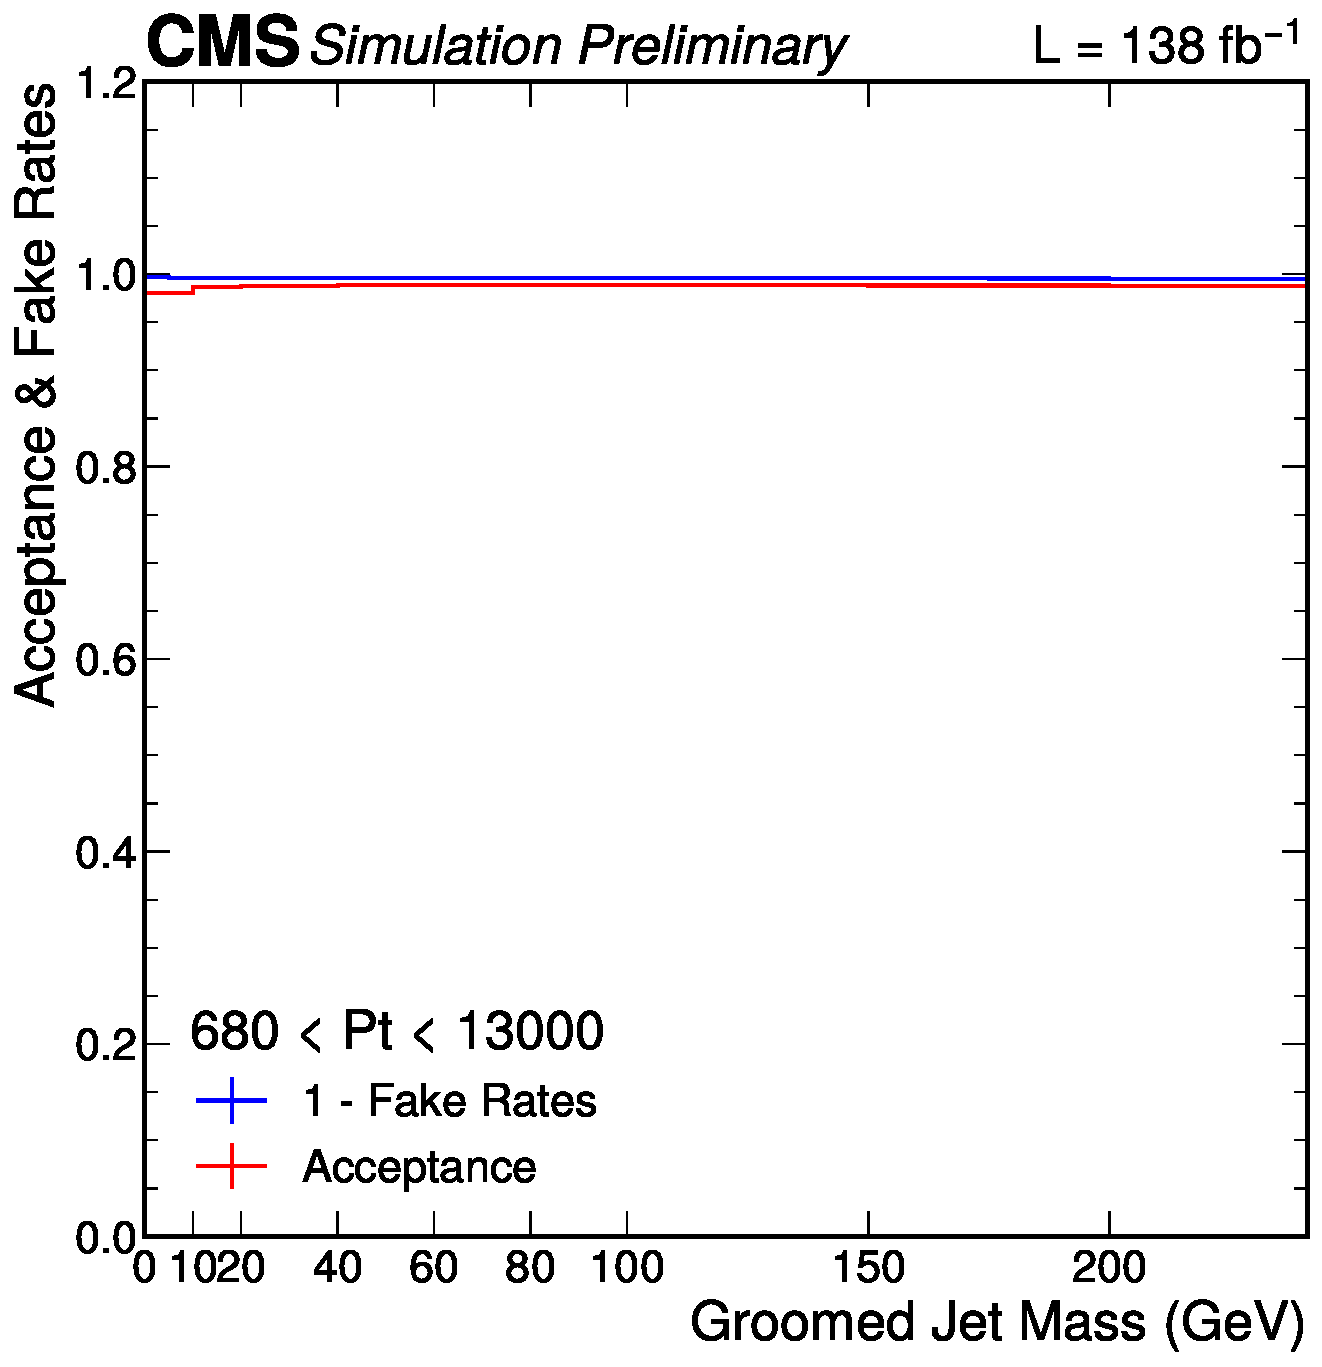
\includegraphics[width=0.45\textwidth]{figures/multijet/dijet/fakerates_groomed_4.pdf}
        \end{subfigure}
	\caption{Fake and acceptance rates as a function of  groomed jet mass for each pt bin for the dijet channel.}
	\label{fig:fakeratesbinned_dijet_g}
      \end{figure}
      
      \begin{figure}[htp!]
	\centering
	\begin{subfigure}
          \centering
          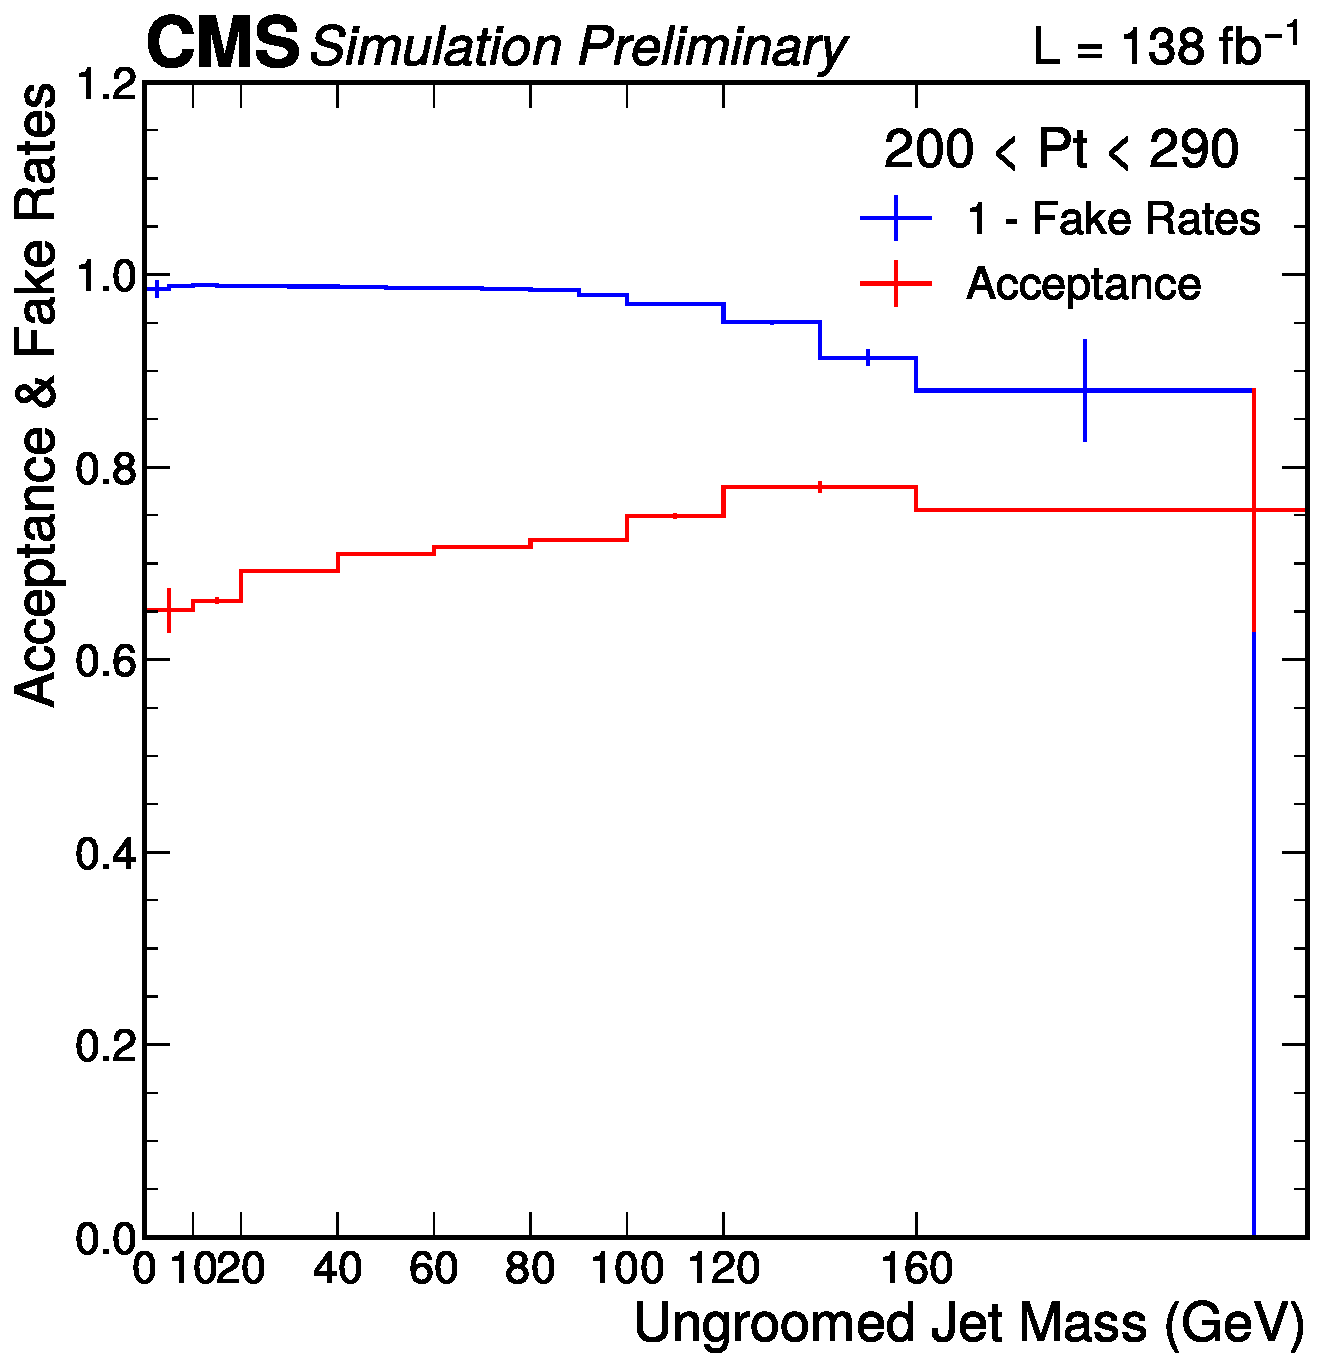
\includegraphics[width=0.45\textwidth]{figures/multijet/trijet/fakerates_ungroomed_0.pdf}
        \end{subfigure}%
        \begin{subfigure}
          \centering
          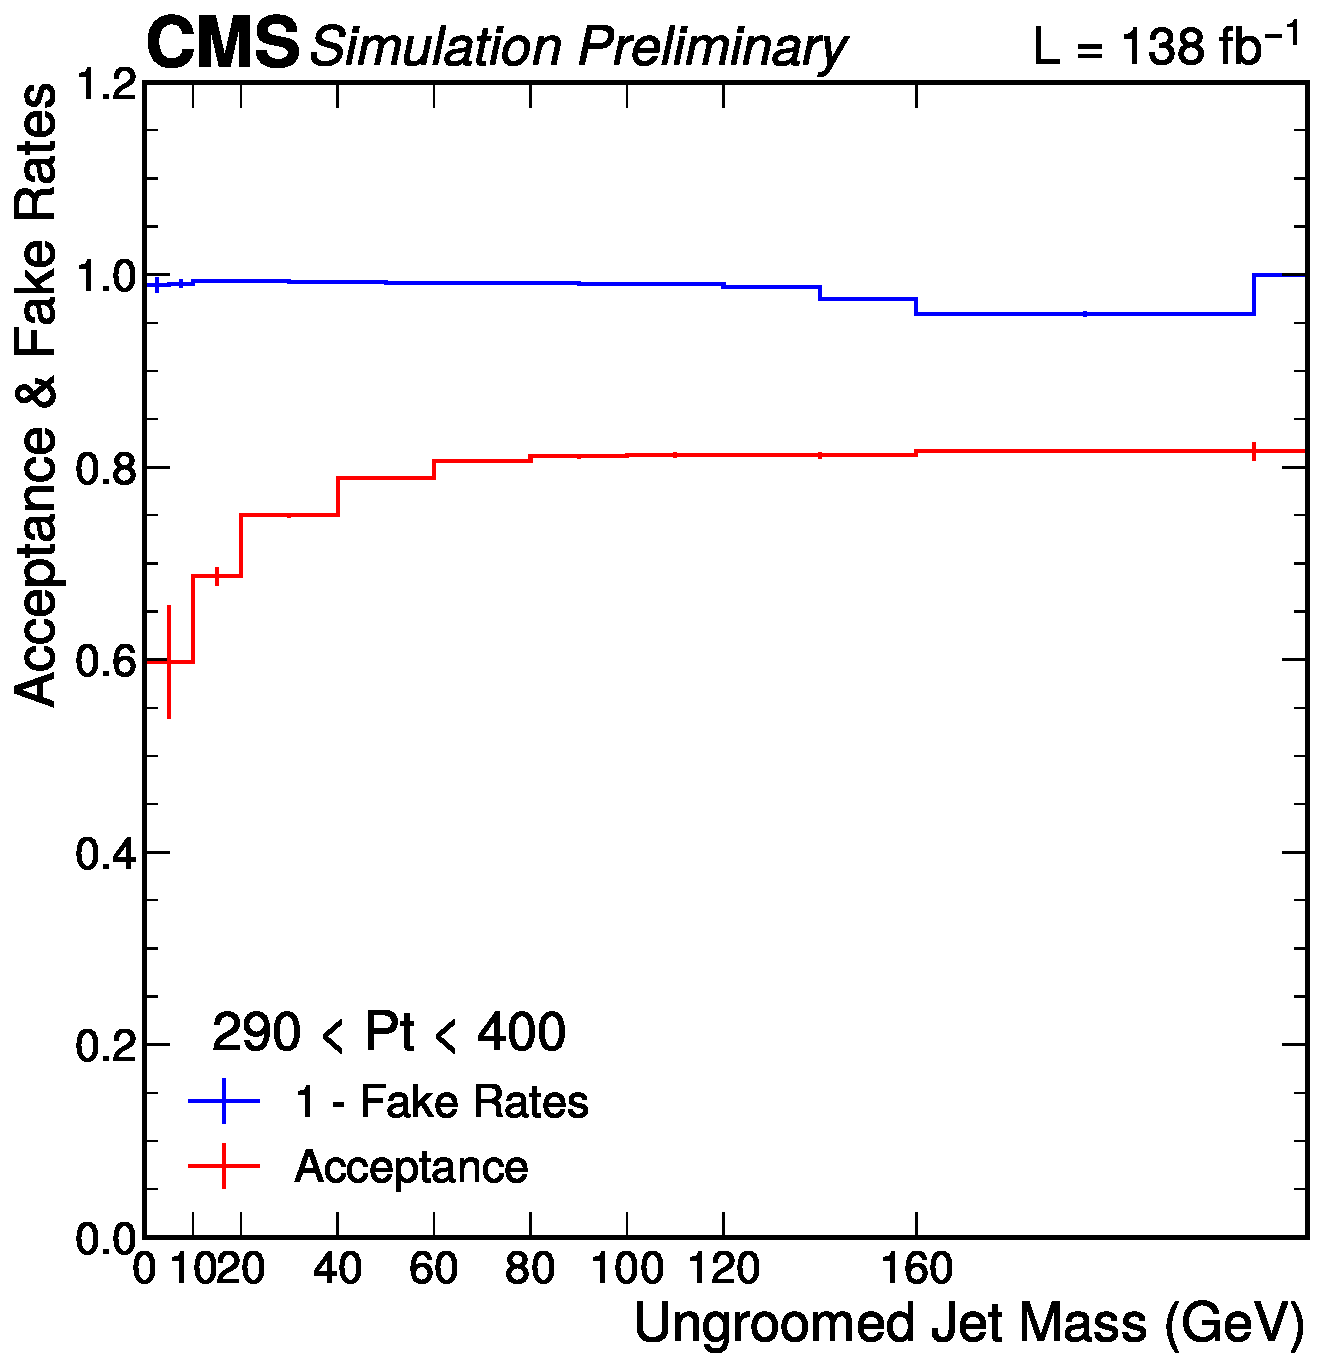
\includegraphics[width=0.45\textwidth]{figures/multijet/trijet/fakerates_ungroomed_1.pdf}
        \end{subfigure}%
        \begin{subfigure}
          \centering
          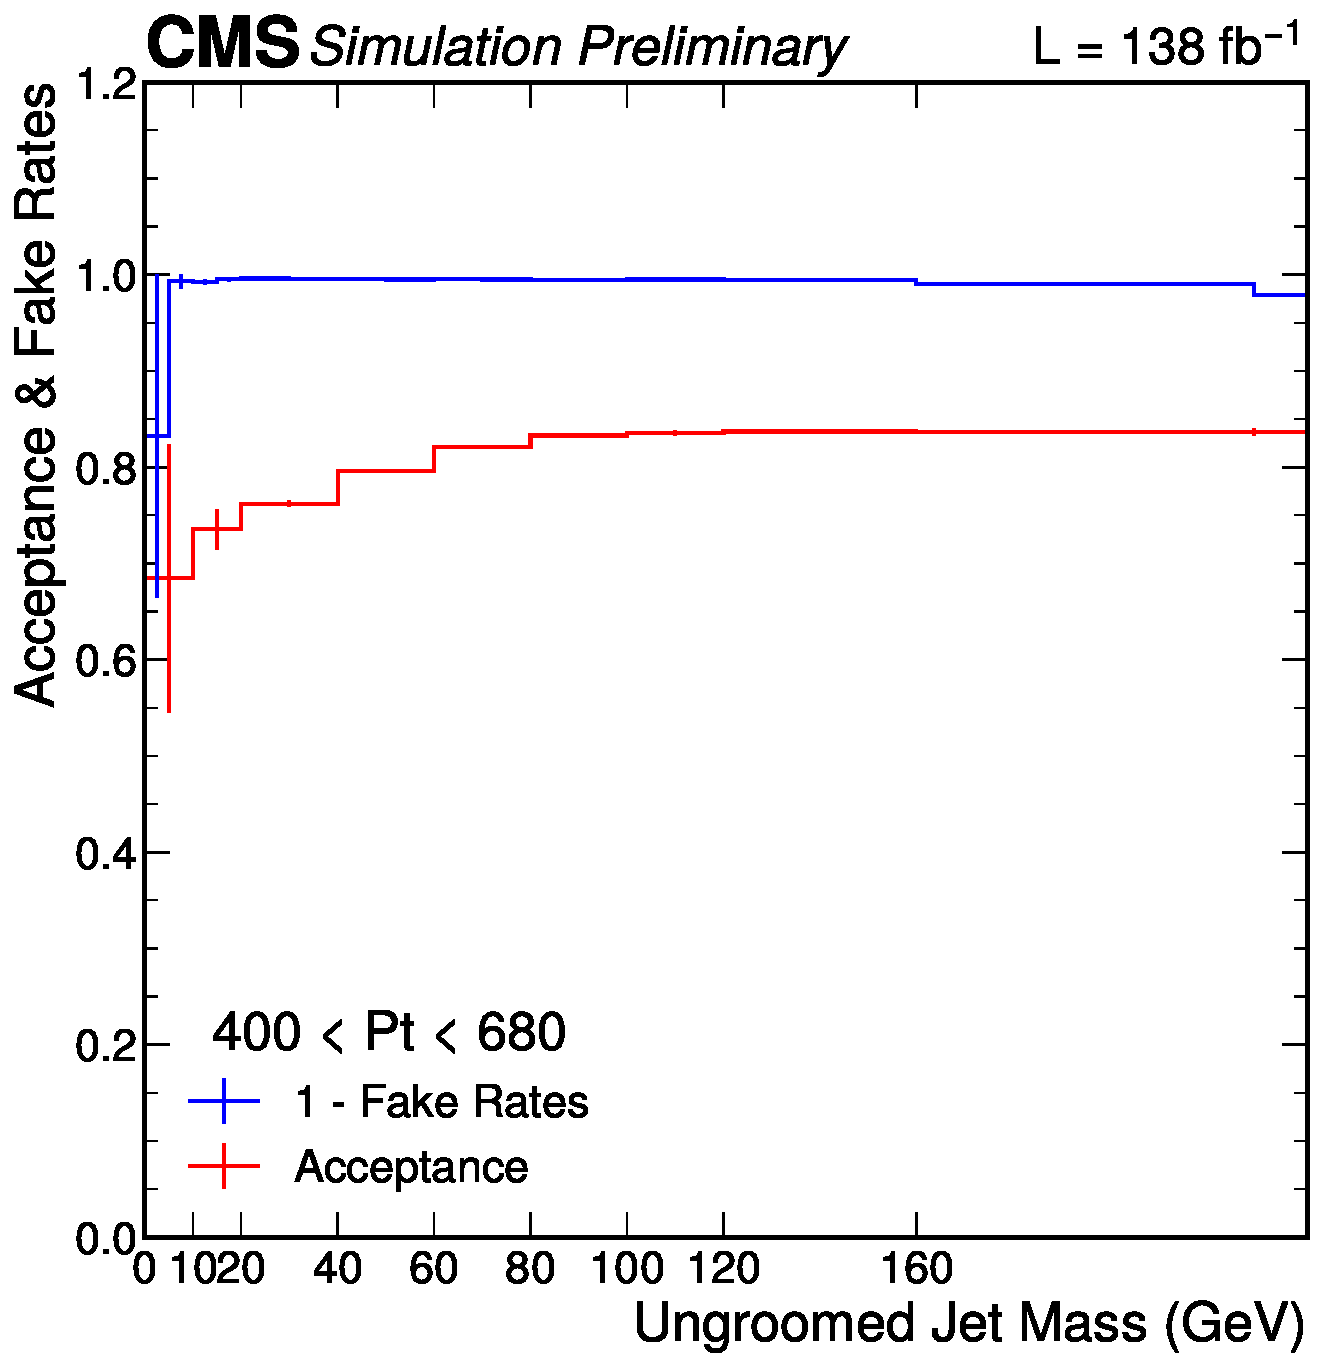
\includegraphics[width=0.45\textwidth]{figures/multijet/trijet/fakerates_ungroomed_2.pdf}
        \end{subfigure}%
        \begin{subfigure}
          \centering
          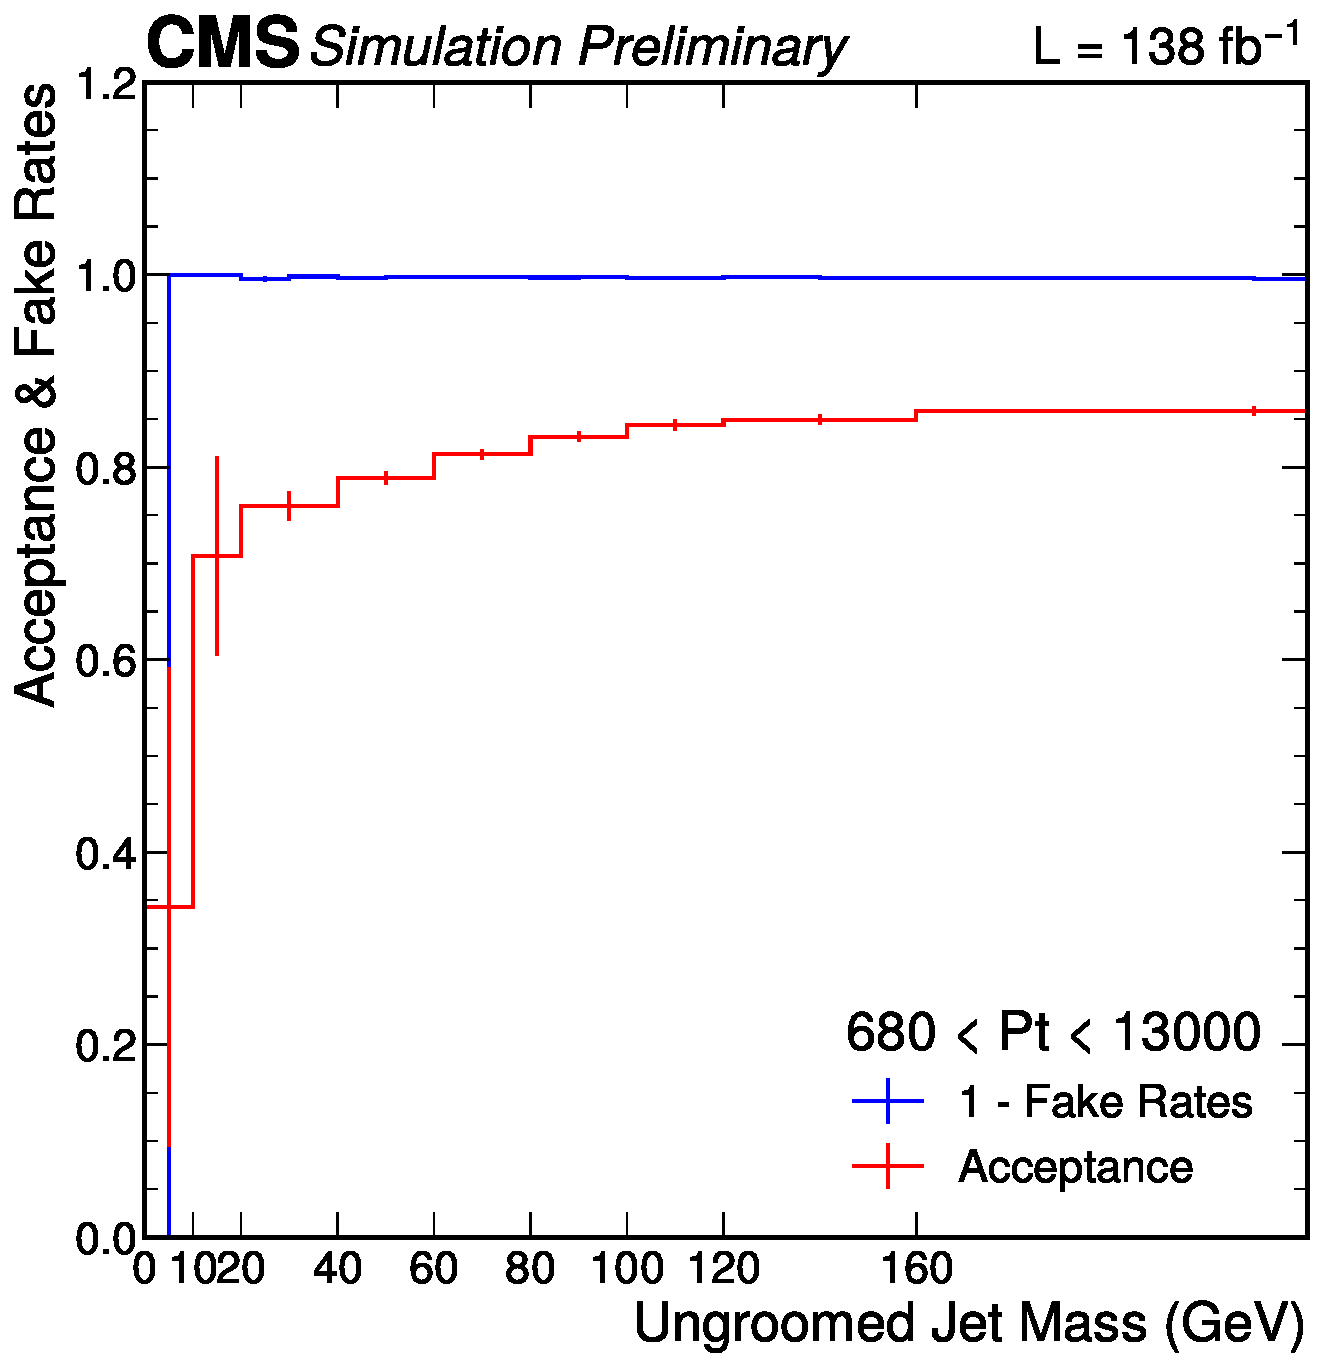
\includegraphics[width=0.45\textwidth]{figures/multijet/trijet/fakerates_ungroomed_3.pdf}
        \end{subfigure}
        \caption{Fake and acceptance rates as a function of ungroomed jet mass for each pt bin for the trijet channel.}
	\label{fig:fakeratesbinned_trijet_u}
      \end{figure}

      \begin{figure}[htp!]
        \begin{subfigure}
          \centering
          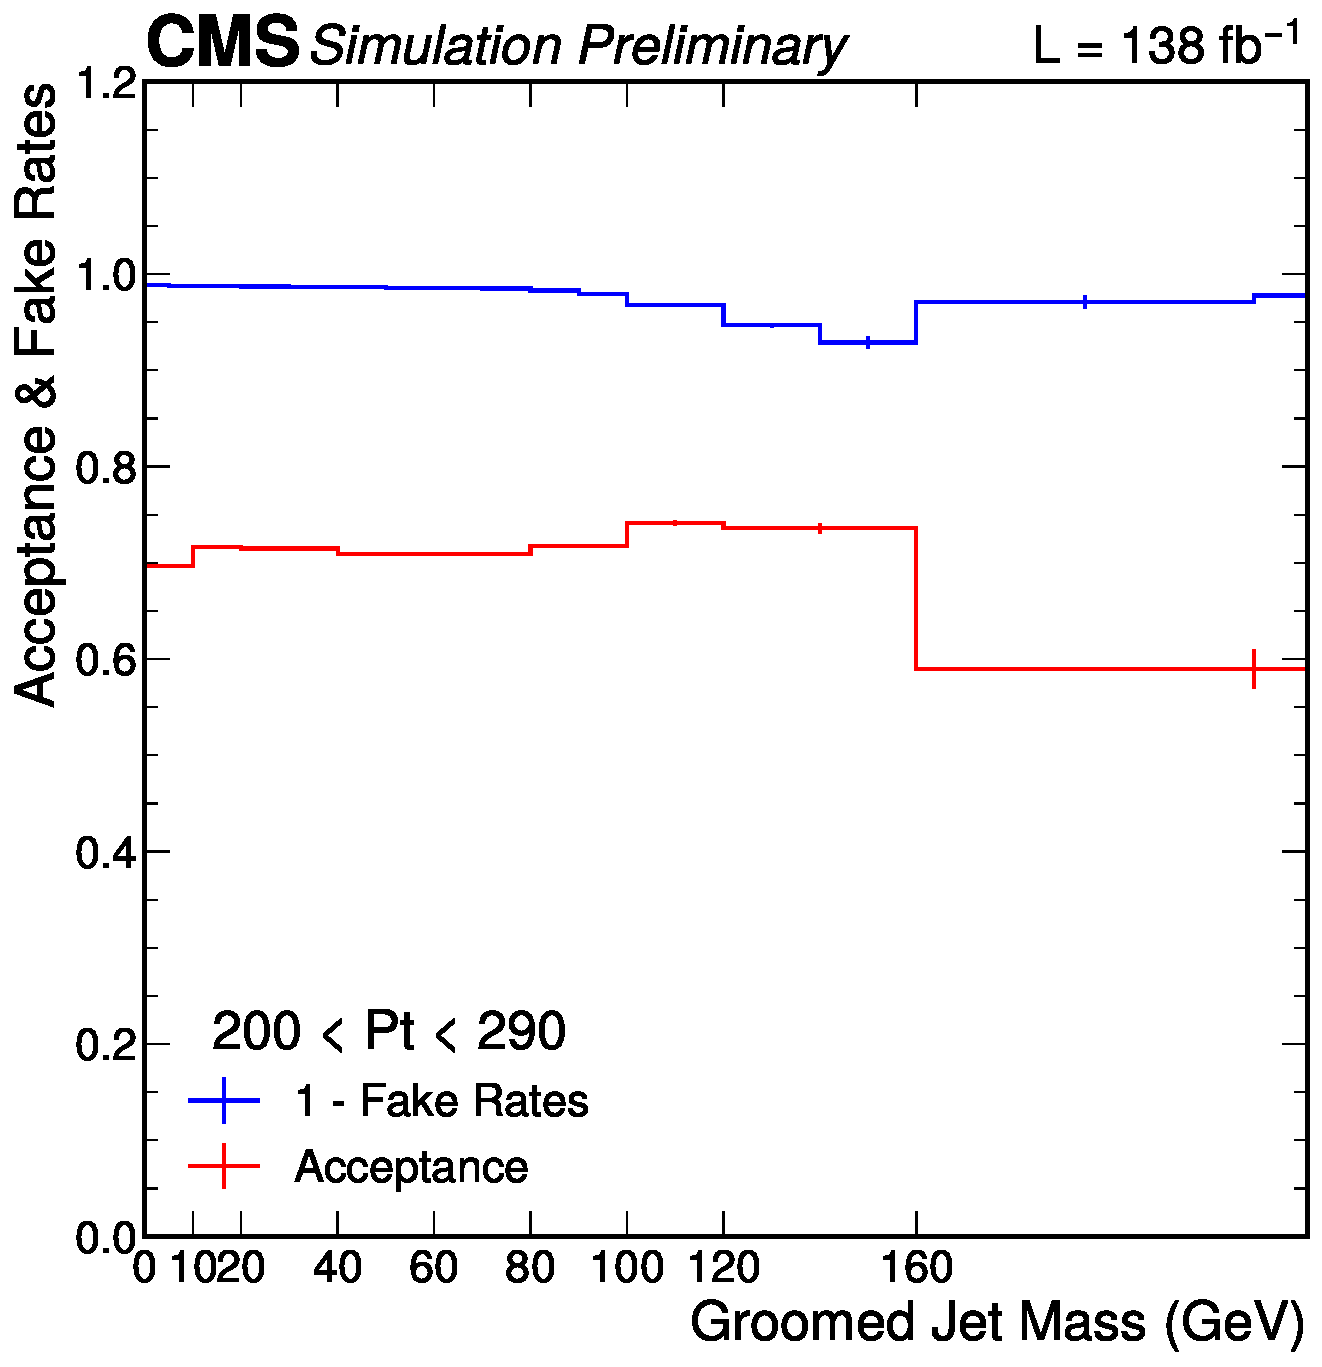
\includegraphics[width=0.45\textwidth]{figures/multijet/trijet/fakerates_groomed_0.pdf}
        \end{subfigure} 
        \begin{subfigure}
          \centering
          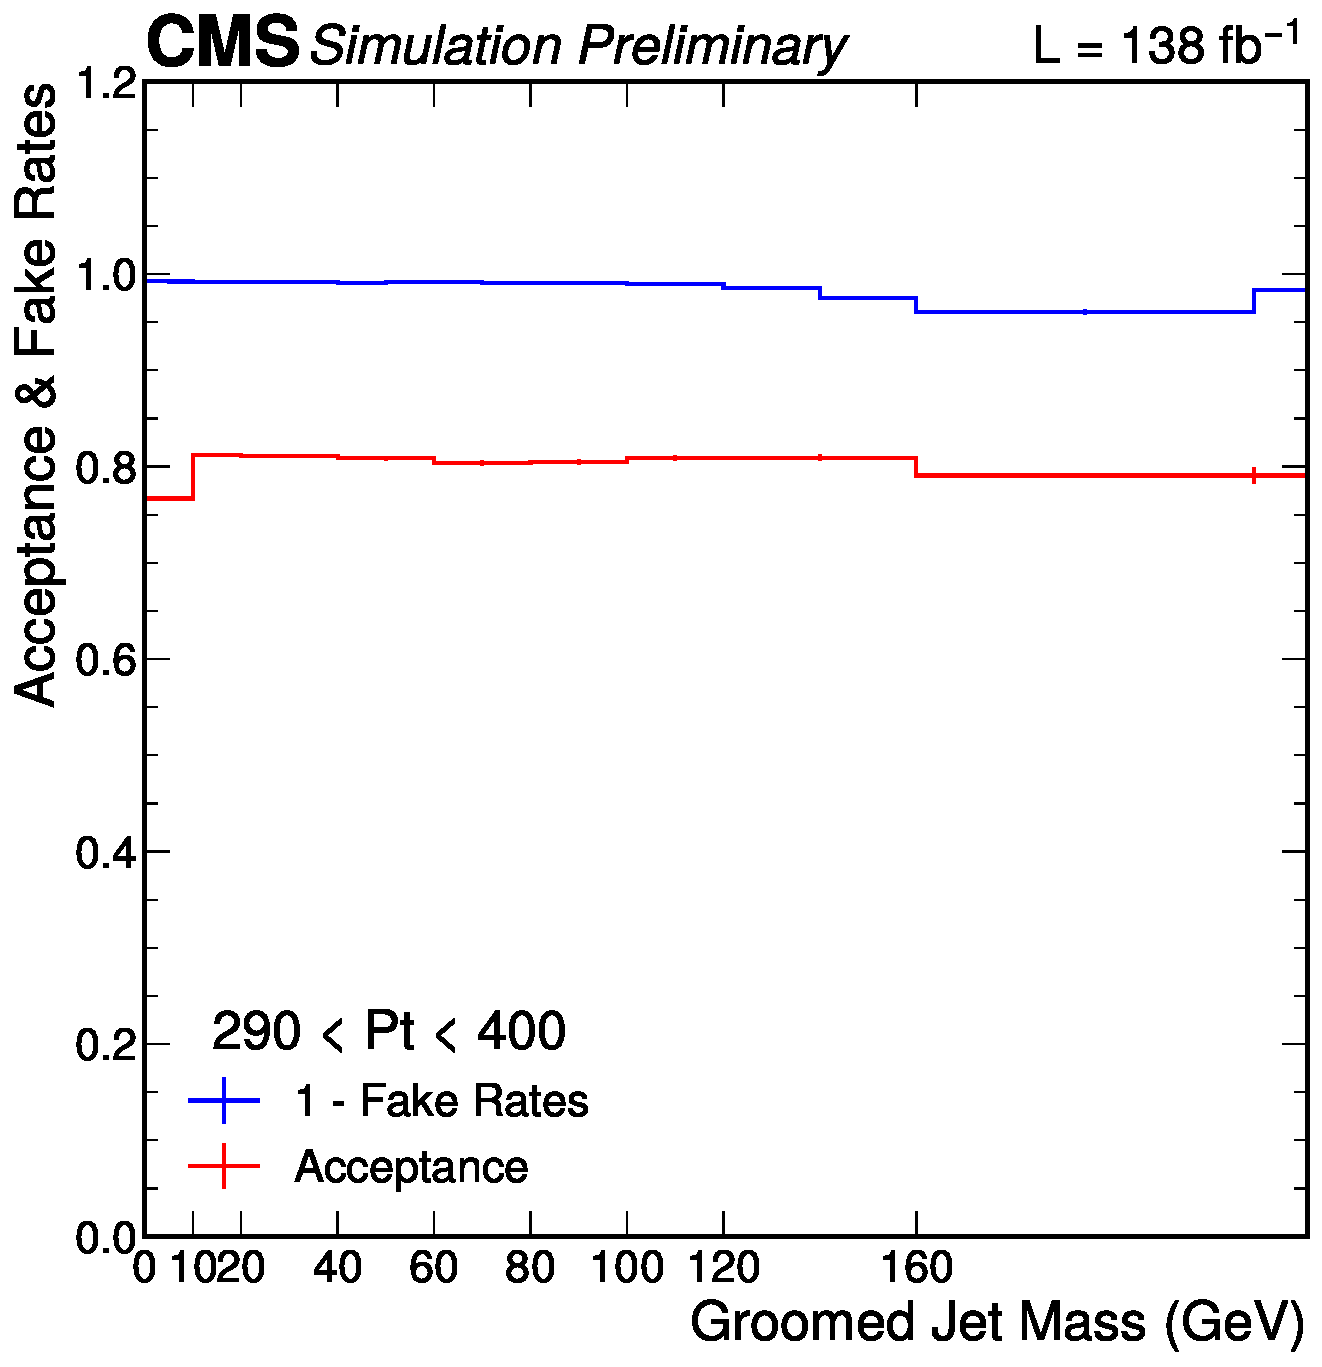
\includegraphics[width=0.45\textwidth]{figures/multijet/trijet/fakerates_groomed_1.pdf}
        \end{subfigure}
        \begin{subfigure}
          \centering
          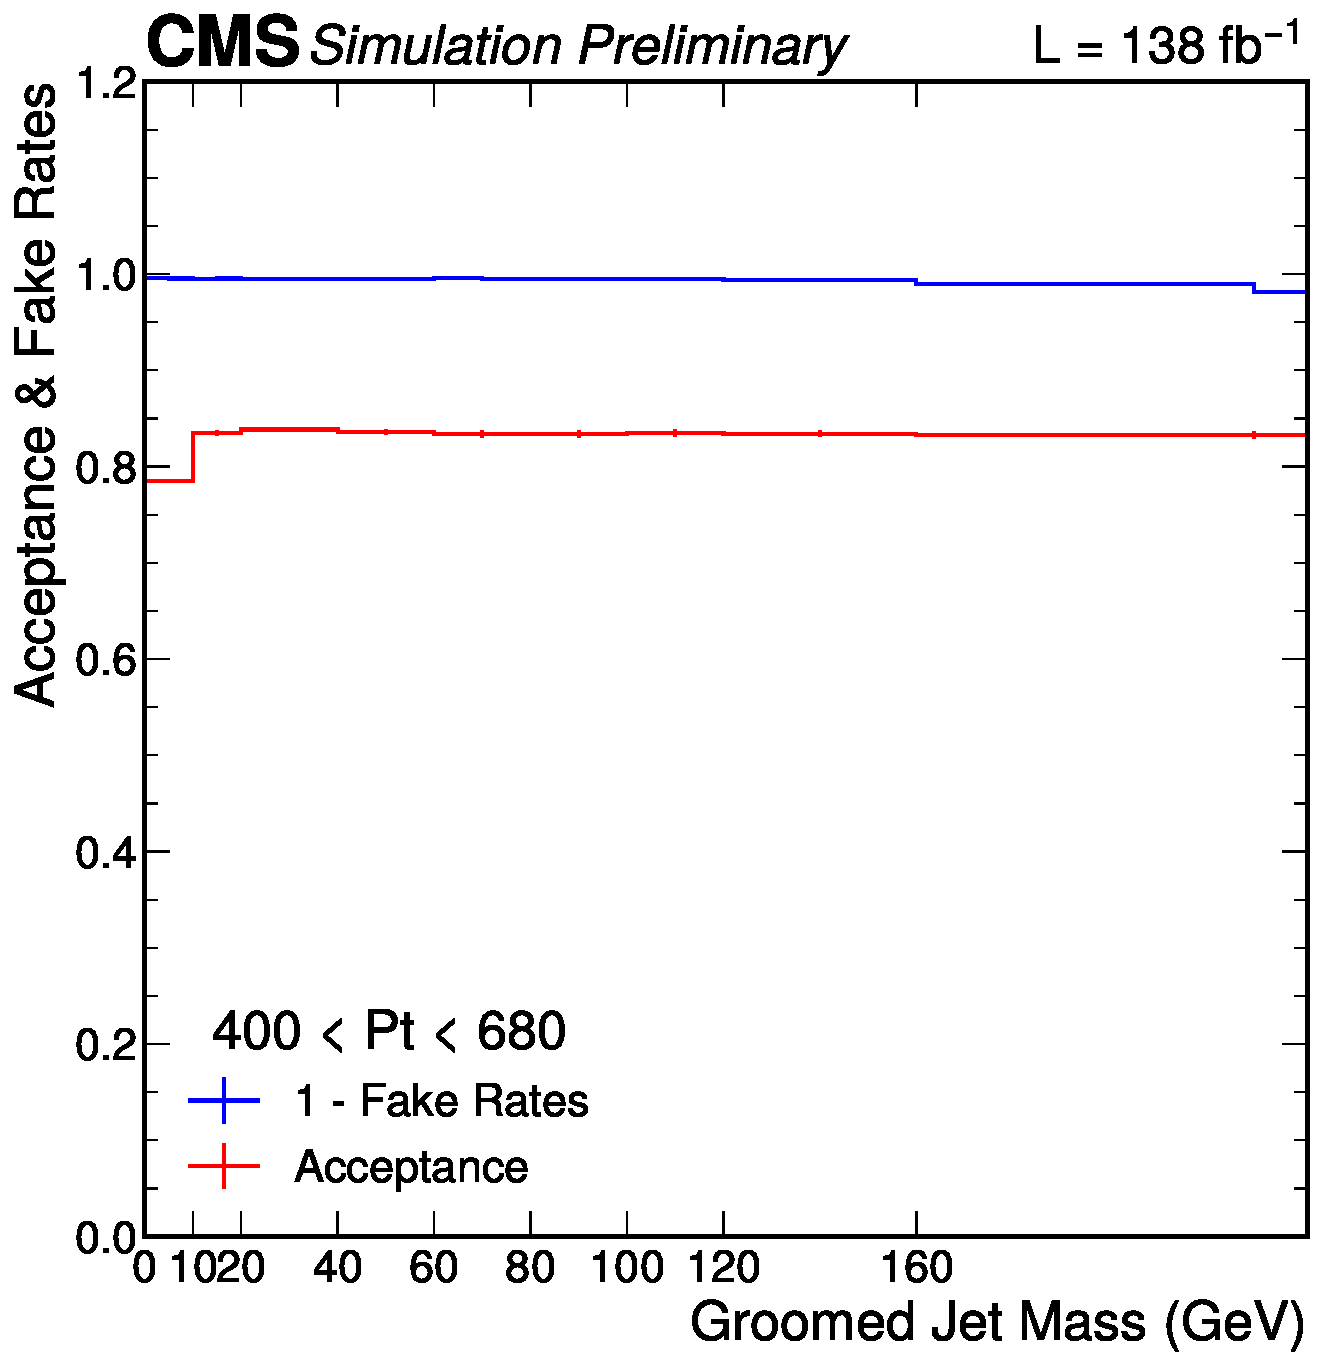
\includegraphics[width=0.45\textwidth]{figures/multijet/trijet/fakerates_groomed_2.pdf}
        \end{subfigure} 
        \begin{subfigure}
          \centering
          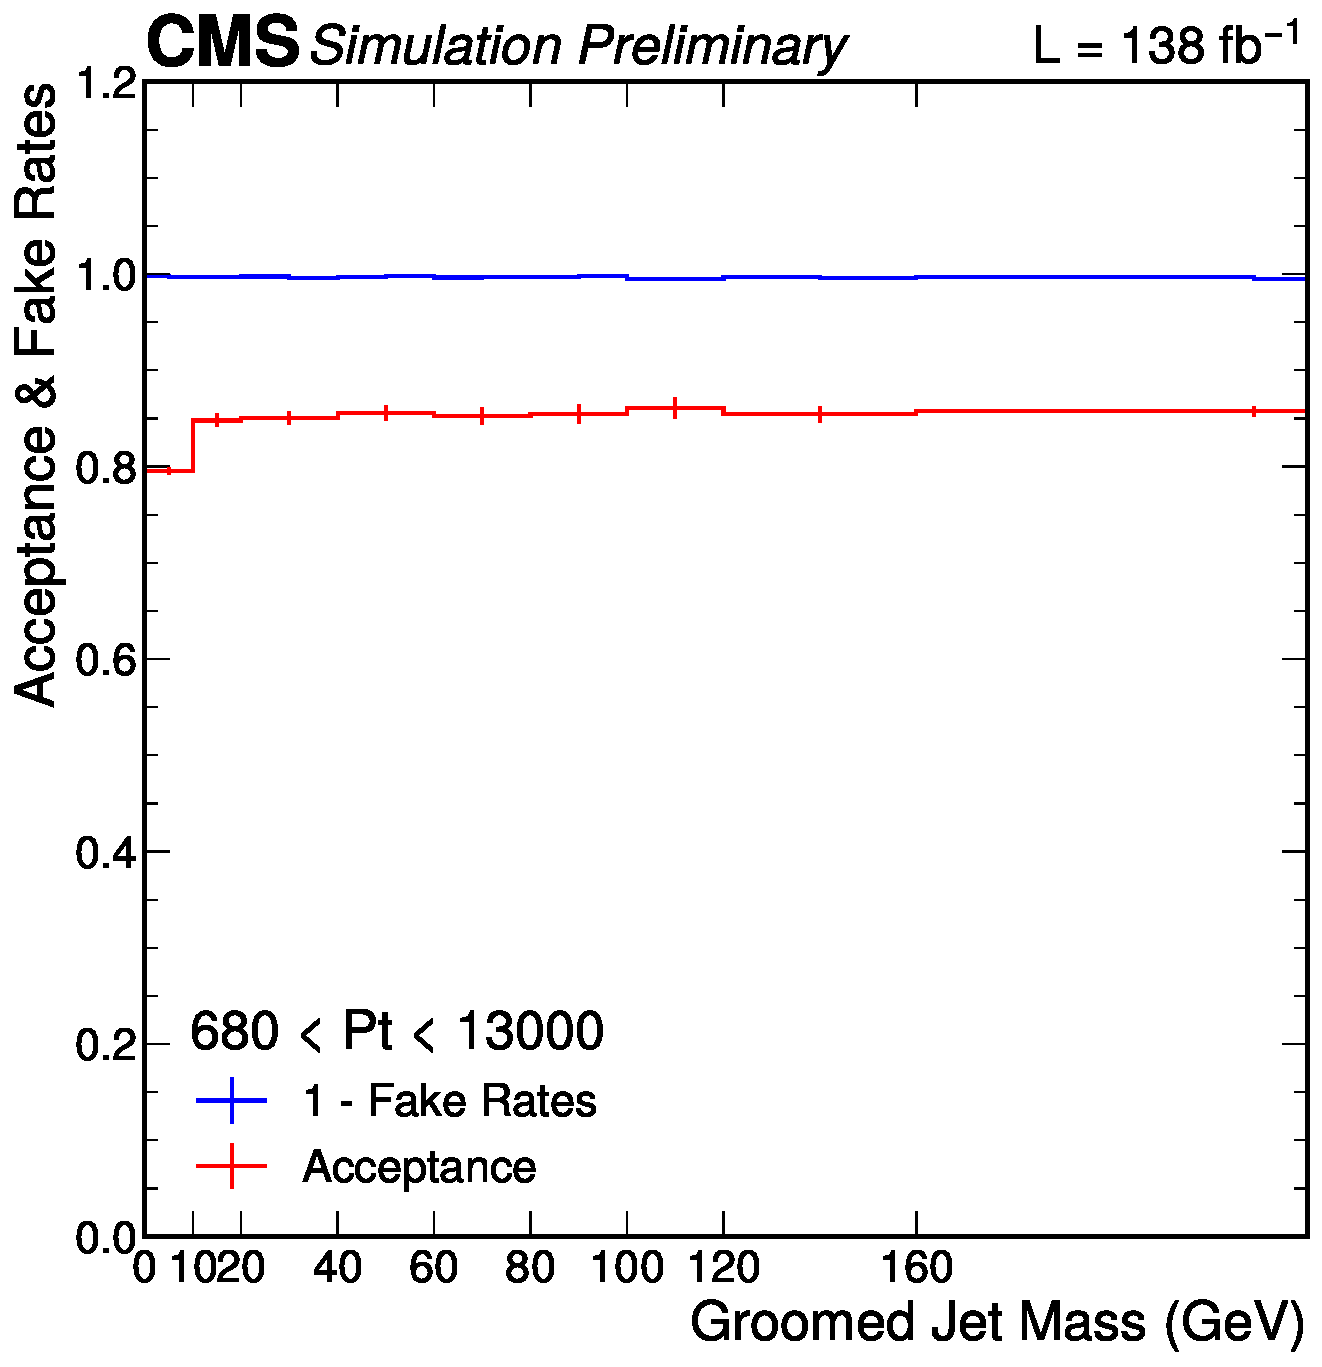
\includegraphics[width=0.45\textwidth]{figures/multijet/trijet/fakerates_groomed_3.pdf}
        \end{subfigure} \\
	\caption{Fake and acceptance rates as a function of groomed jet mass for each pt bin for the trijet channel.}
	\label{fig:fakeratesbinned_trijet_g}
      \end{figure}
      
      \subsection{Closure and bias tests}
      The simplest consistency check on whether the unfolding is stable is done by unfolding the reconstructed events of the same simulated data that was used to produce the response matrices. The output of this test should be identical to the generator level distribution. We can see in Figures \ref{fig:dijetclosurebinned_u} - \ref{fig:trijetclosurebinned_g} that we have perfect self-closure.\\
        The next test is to unfold a sample simulated with a different generator with the same Pythia8 response matrix and see how successful it is to show that the response matrix is not overly biased by the model used to produce it. We do this by unfolding Madgraph+HERWIG samples using the same Madgraph+Pythia8 response matrix that will be used to unfold the data. The result of this test can be seen in Figures \ref{fig:dijetherwigclosurebinned_u} - \ref{fig:trijetherwigclosurebinned_g} and from these we see that the for the majority of the bins Herwig sample has agreeable results with the truth after unfolding showing that our matrix is not overly biased towards one model. We see the unfolding break down in the highest bin of the trijet sample, but as can be seen in Figure \ref{fig:herwig}, we see that the \pt sprecta vary greatly between the two models. We account for any biases introduced by the model by including a parton shower and shape uncertainty using the difference between the normalized Pythia and Herwig samples as a systematic uncertainty as described in Sec. \ref{systematics}.
      
      \begin{figure}[htp!]
	\centering
	\begin{subfigure}
          \centering
          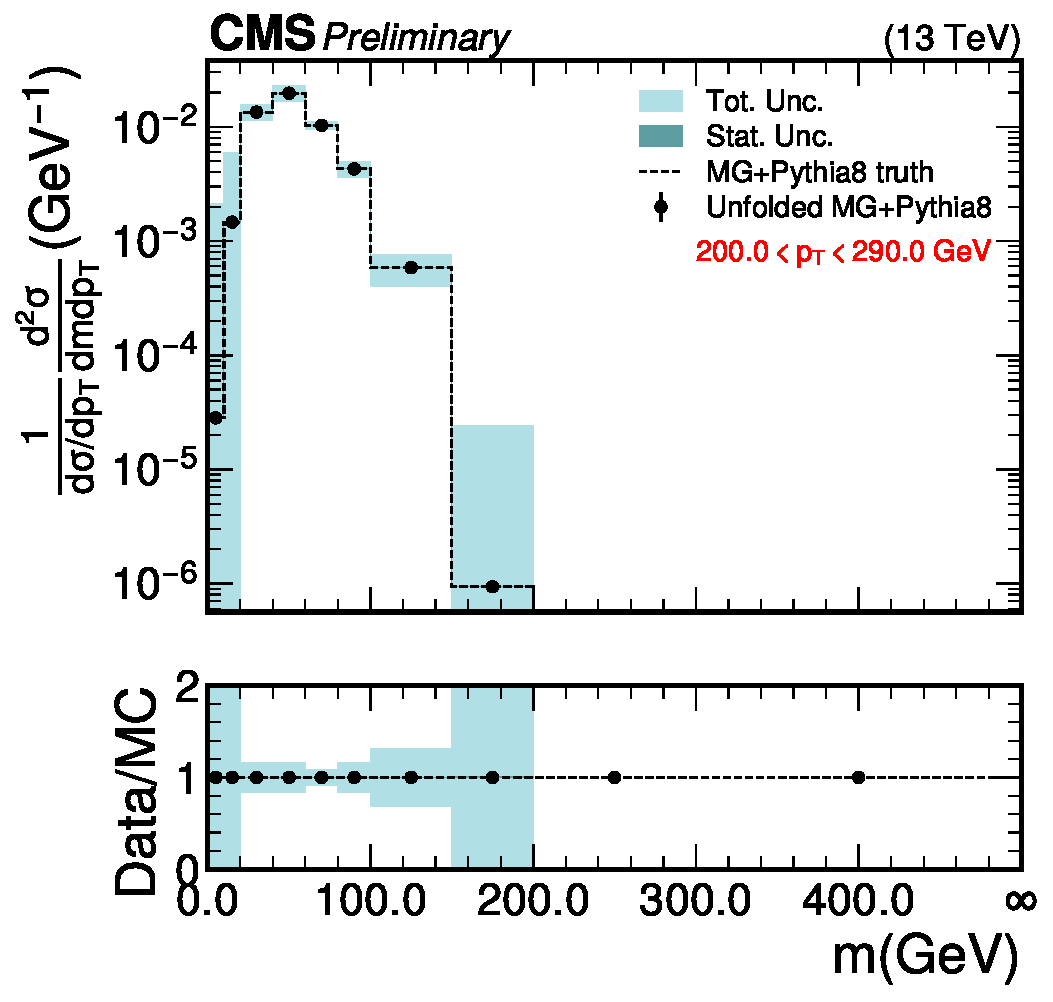
\includegraphics[width=0.45\textwidth]{figures/multijet/unfolding/dijet/closure_binnedResult_ungroomed_0.pdf}
        \end{subfigure}%
        \begin{subfigure}
          \centering
          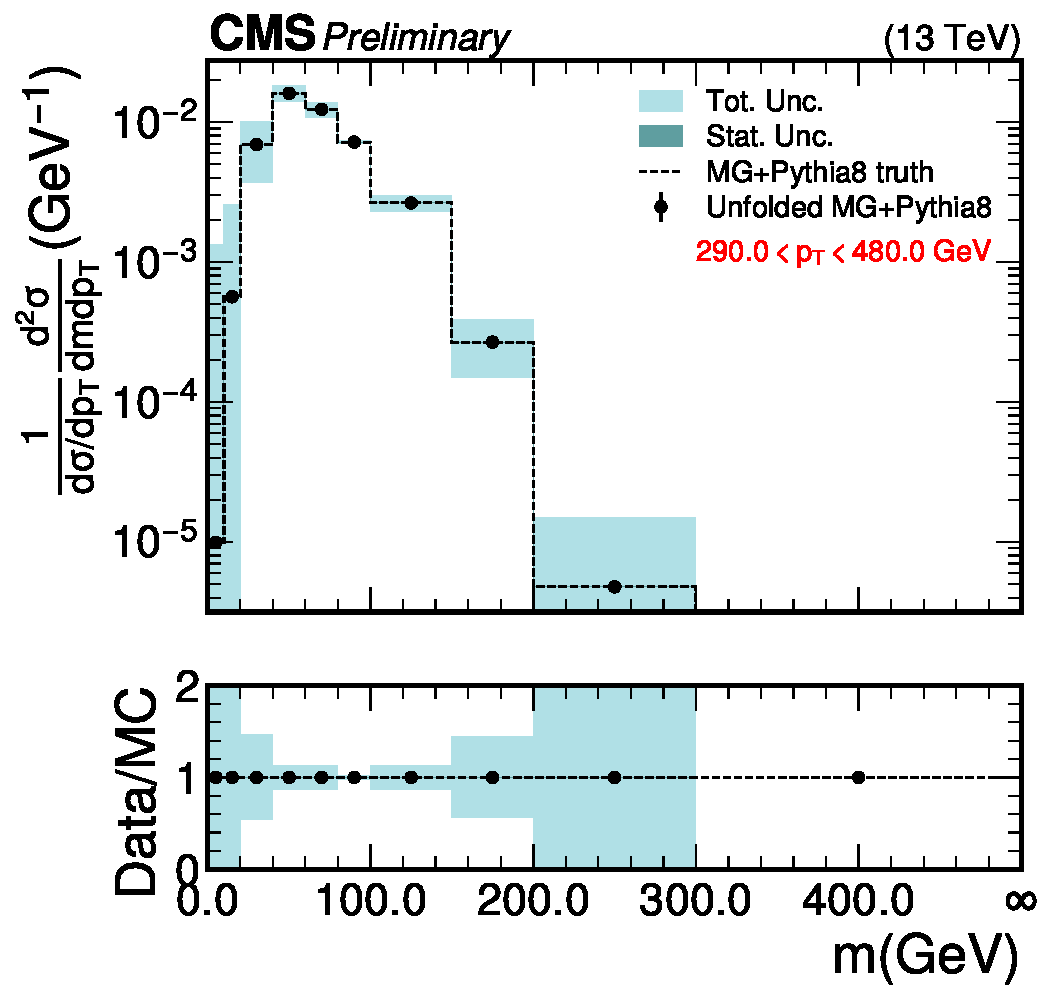
\includegraphics[width=0.45\textwidth]{figures/multijet/unfolding/dijet/closure_binnedResult_ungroomed_1.pdf}
        \end{subfigure}%
        \begin{subfigure}
          \centering
          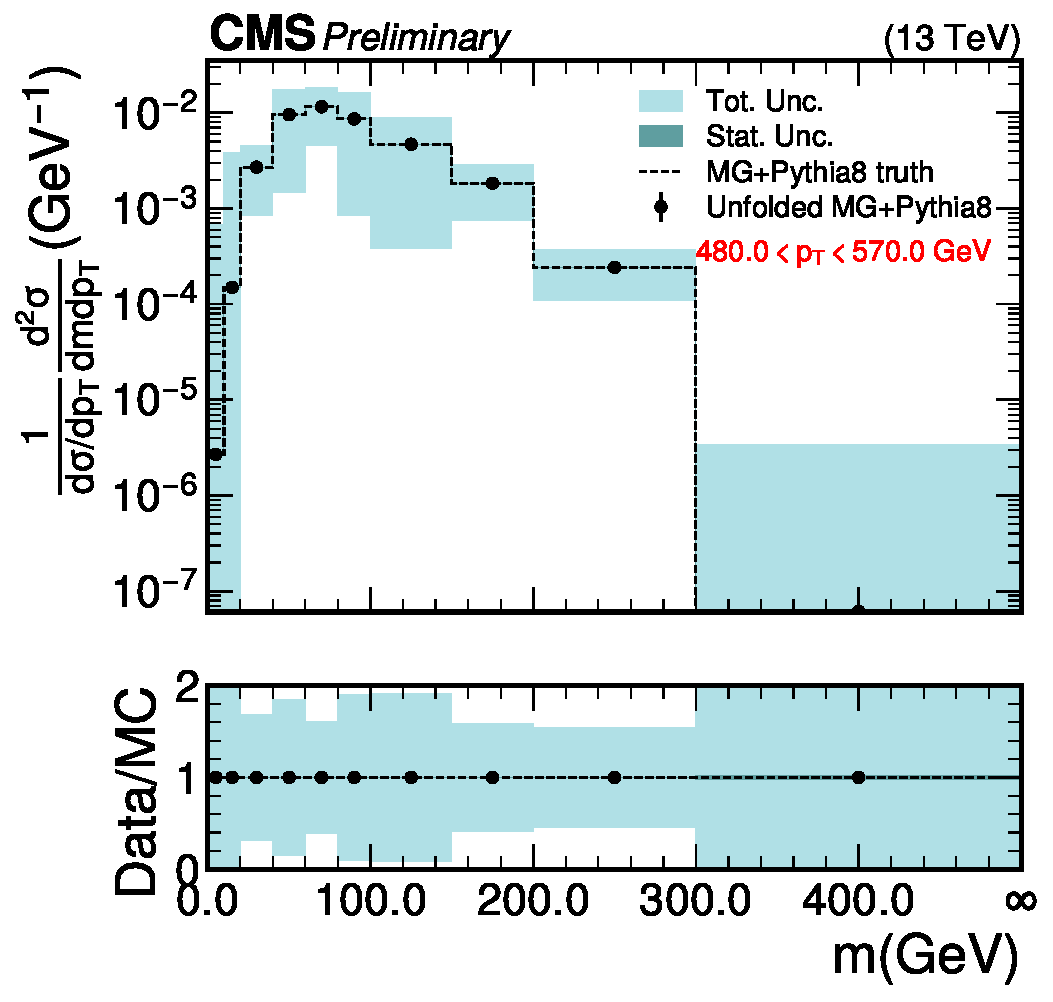
\includegraphics[width=0.45\textwidth]{figures/multijet/unfolding/dijet/closure_binnedResult_ungroomed_2.pdf}
        \end{subfigure}%
        \begin{subfigure}
          \centering
          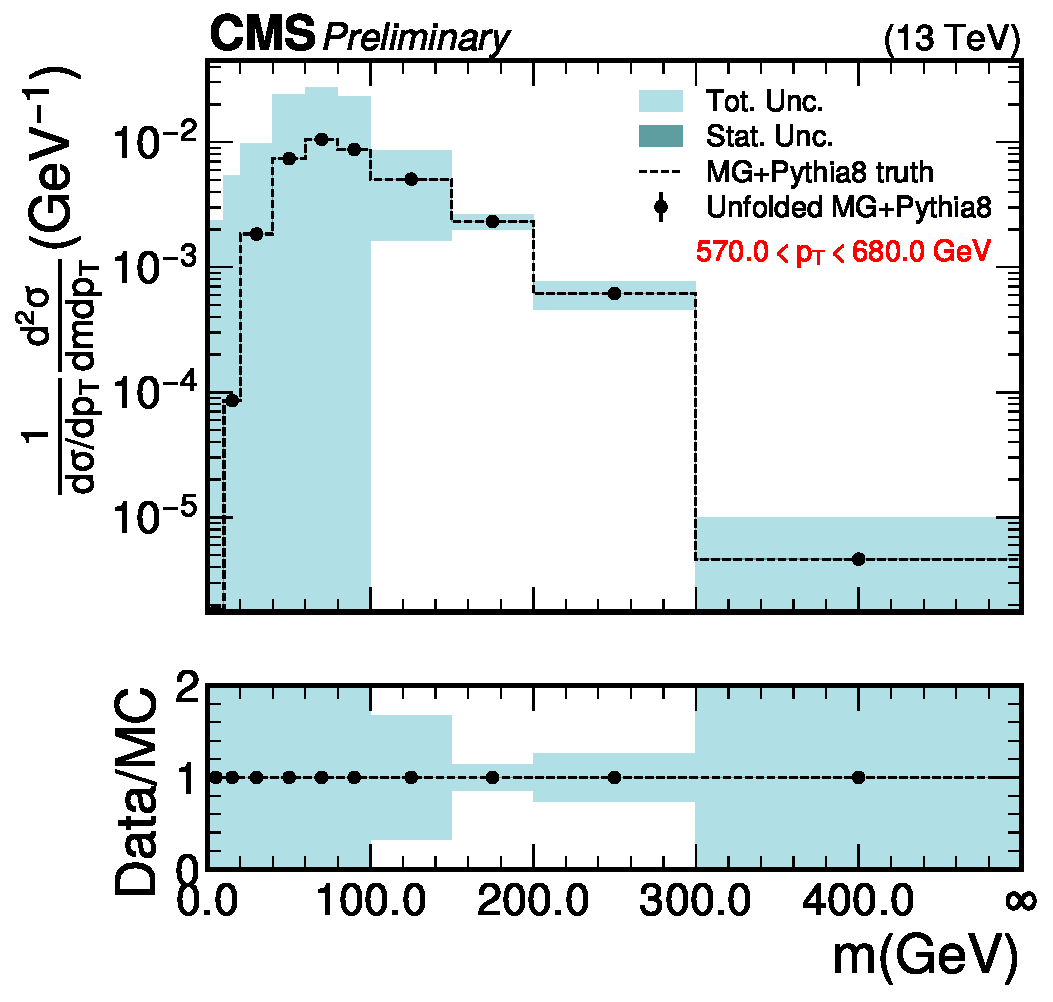
\includegraphics[width=0.45\textwidth]{figures/multijet/unfolding/dijet/closure_binnedResult_ungroomed_3.pdf}
        \end{subfigure}
        \begin{subfigure}
          \centering
          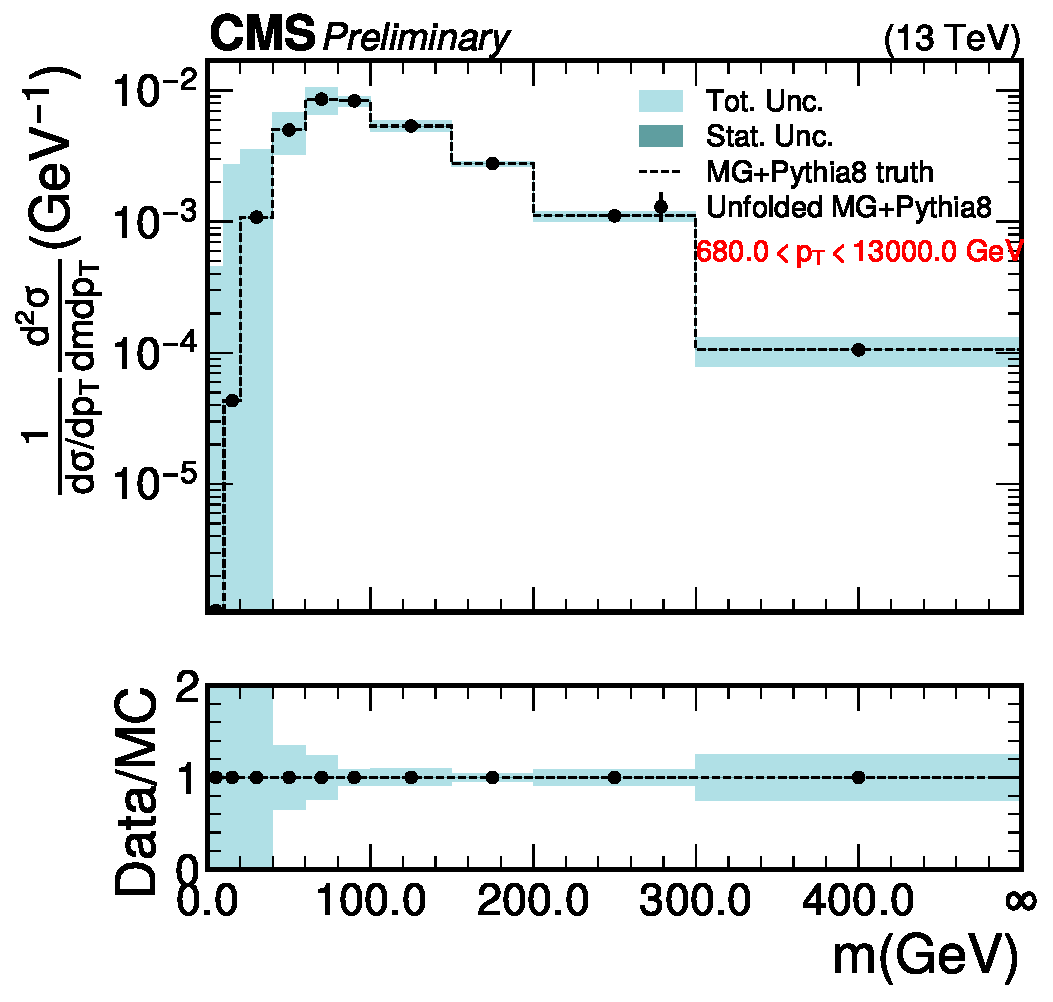
\includegraphics[width=0.45\textwidth]{figures/multijet/unfolding/dijet/closure_binnedResult_ungroomed_4.pdf}
        \end{subfigure}
        \caption{Dijet self-closure test results for the ungroomed jet mass.}
	\label{fig:dijetclosurebinned_u}
      \end{figure}

      \begin{figure}[htp!]
        \begin{subfigure}
          \centering
          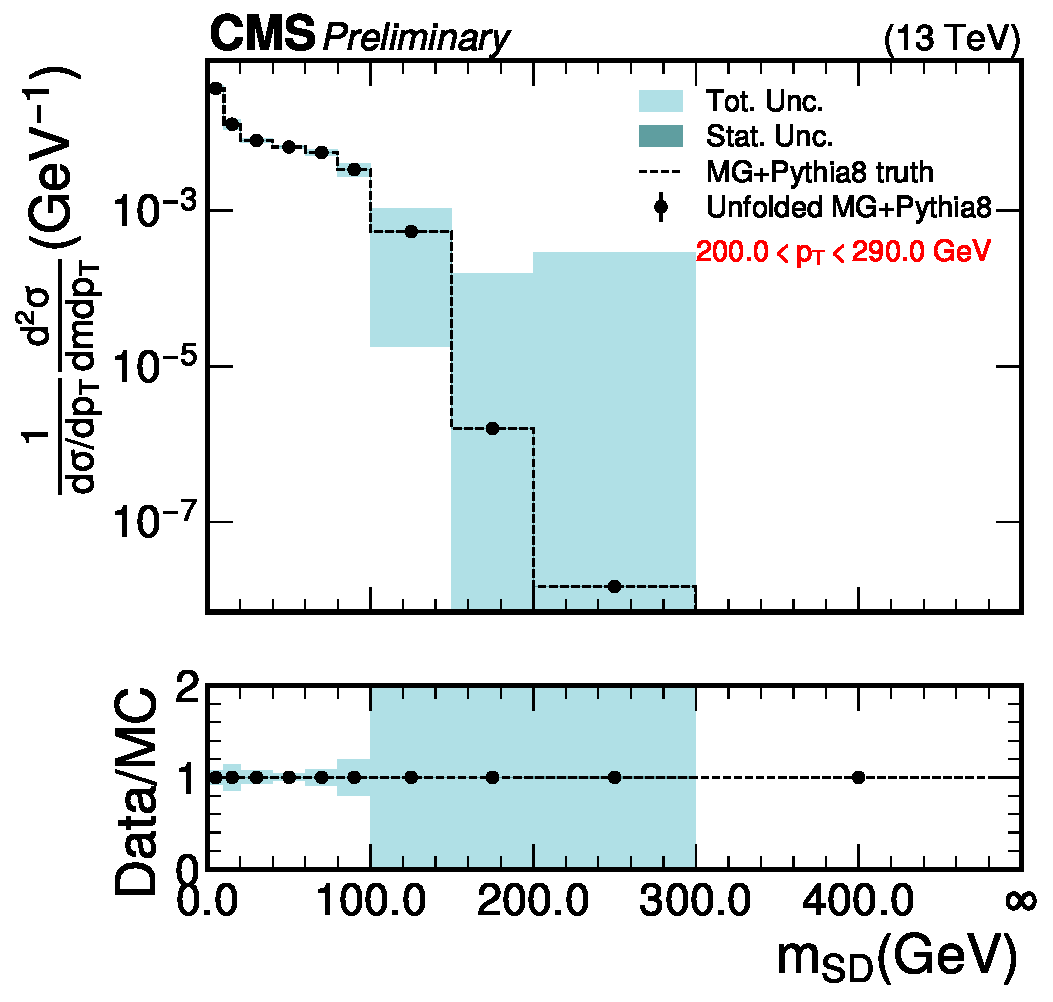
\includegraphics[width=0.45\textwidth]{figures/multijet/unfolding/dijet/closure_binnedResult_groomed_0.pdf}
        \end{subfigure} 
        \begin{subfigure}
          \centering
          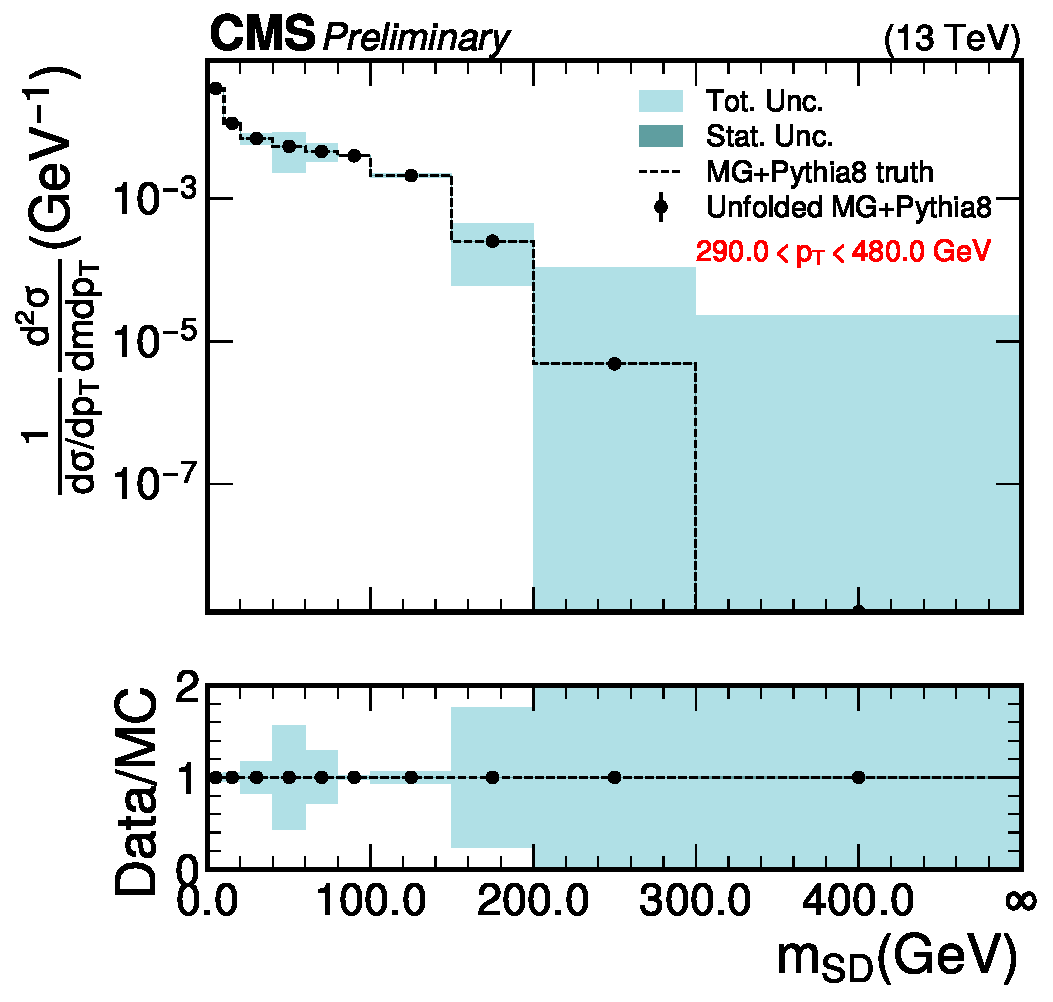
\includegraphics[width=0.45\textwidth]{figures/multijet/unfolding/dijet/closure_binnedResult_groomed_1.pdf}
        \end{subfigure}
        \begin{subfigure}
          \centering
          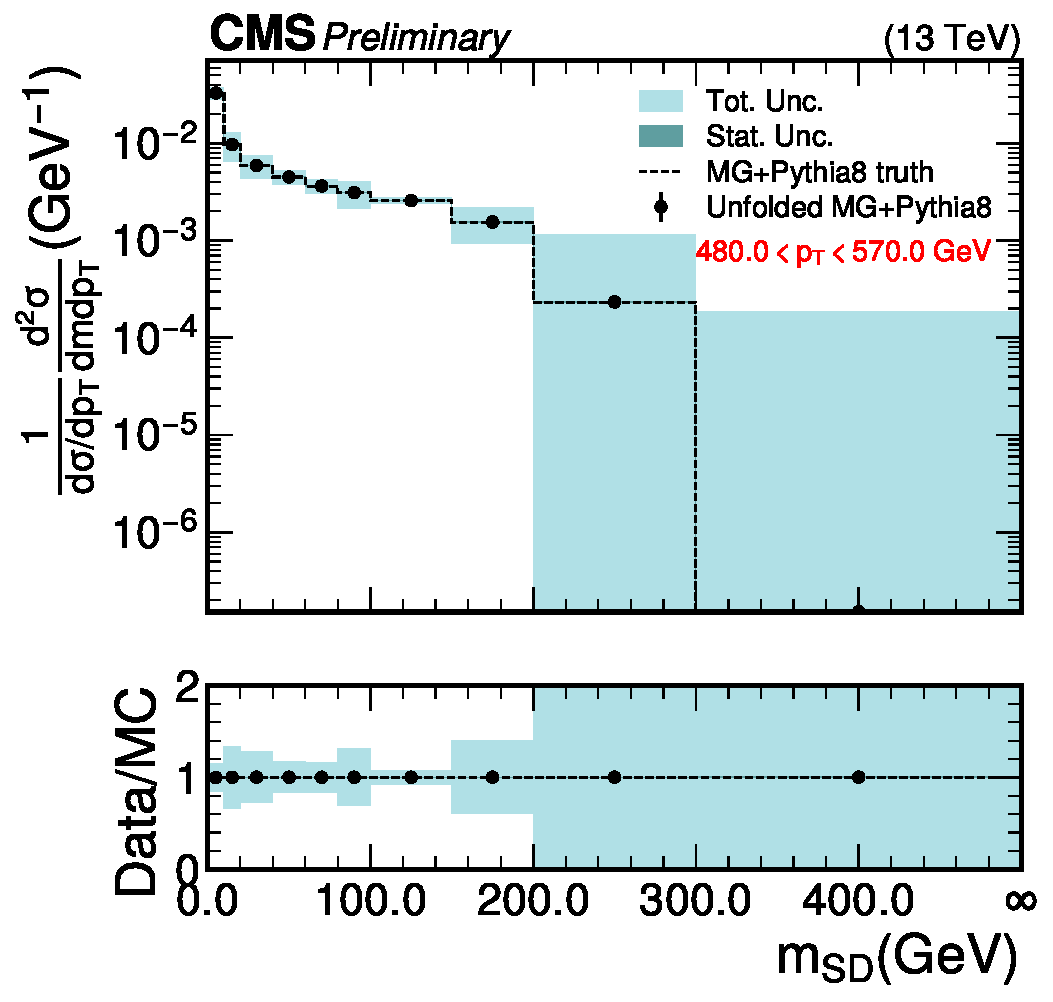
\includegraphics[width=0.45\textwidth]{figures/multijet/unfolding/dijet/closure_binnedResult_groomed_2.pdf}
        \end{subfigure} 
        \begin{subfigure}
          \centering
          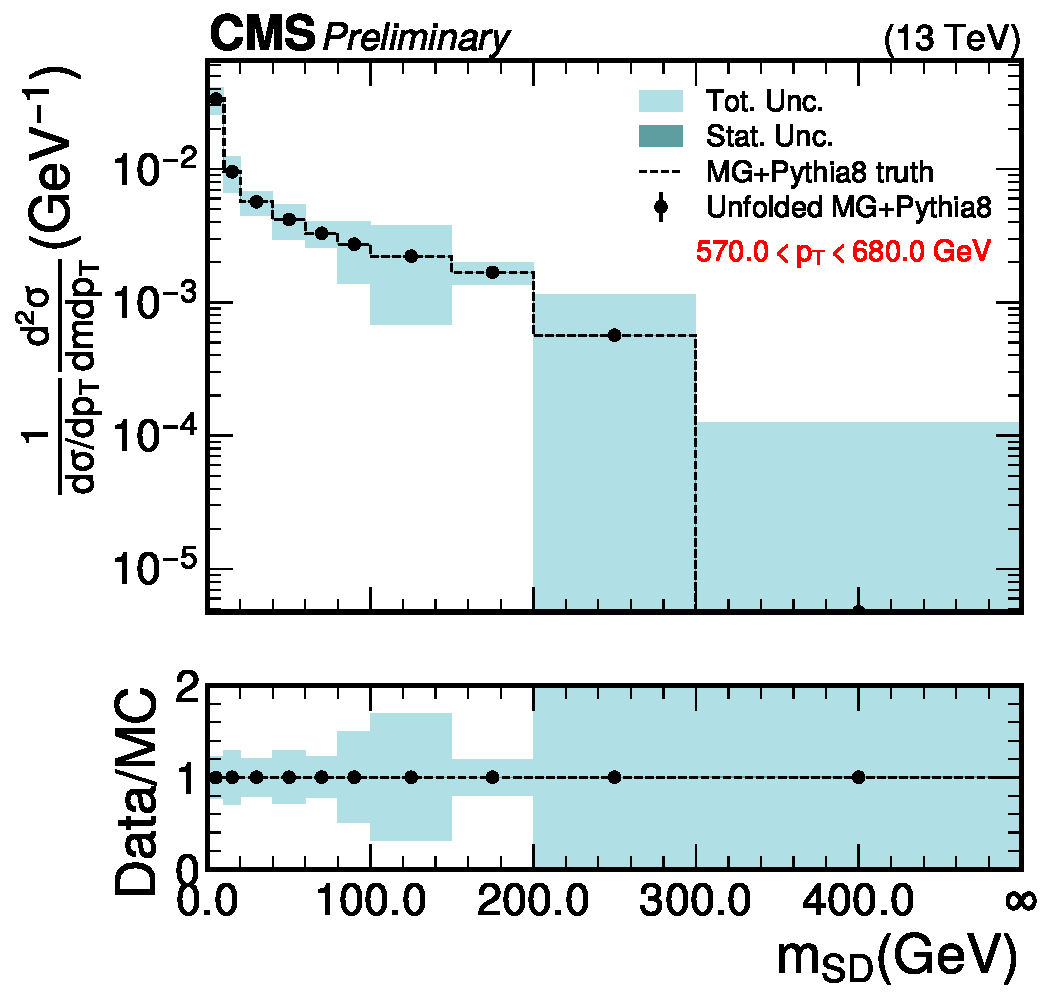
\includegraphics[width=0.45\textwidth]{figures/multijet/unfolding/dijet/closure_binnedResult_groomed_3.pdf}
        \end{subfigure}
        \begin{subfigure}
          \centering
          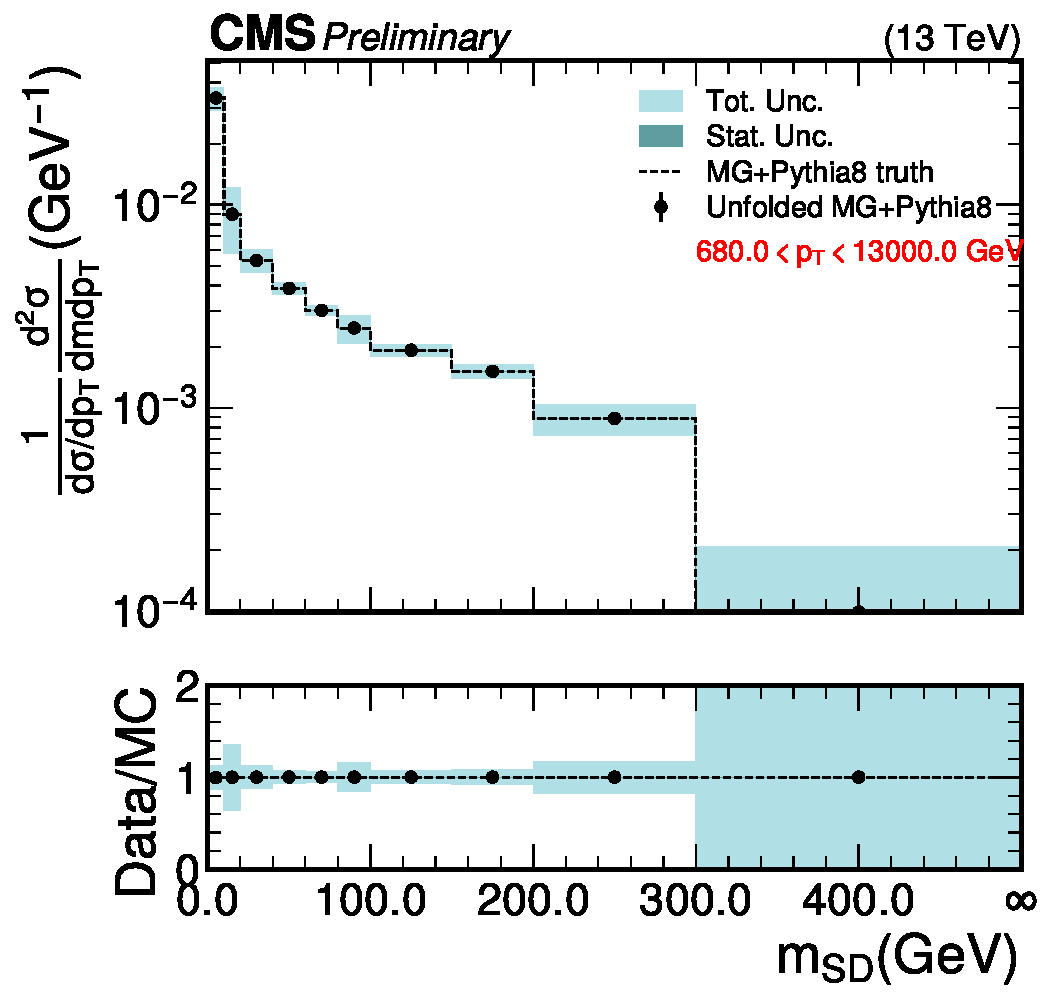
\includegraphics[width=0.45\textwidth]{figures/multijet/unfolding/dijet/closure_binnedResult_groomed_4.pdf}
        \end{subfigure}\\
	\caption{Dijet self-closure test results for the groomed jet mass.}
	\label{fig:dijetclosurebinned_g}
      \end{figure}
      
      \begin{figure}[htp!]
	\centering
	\begin{subfigure}
          \centering
          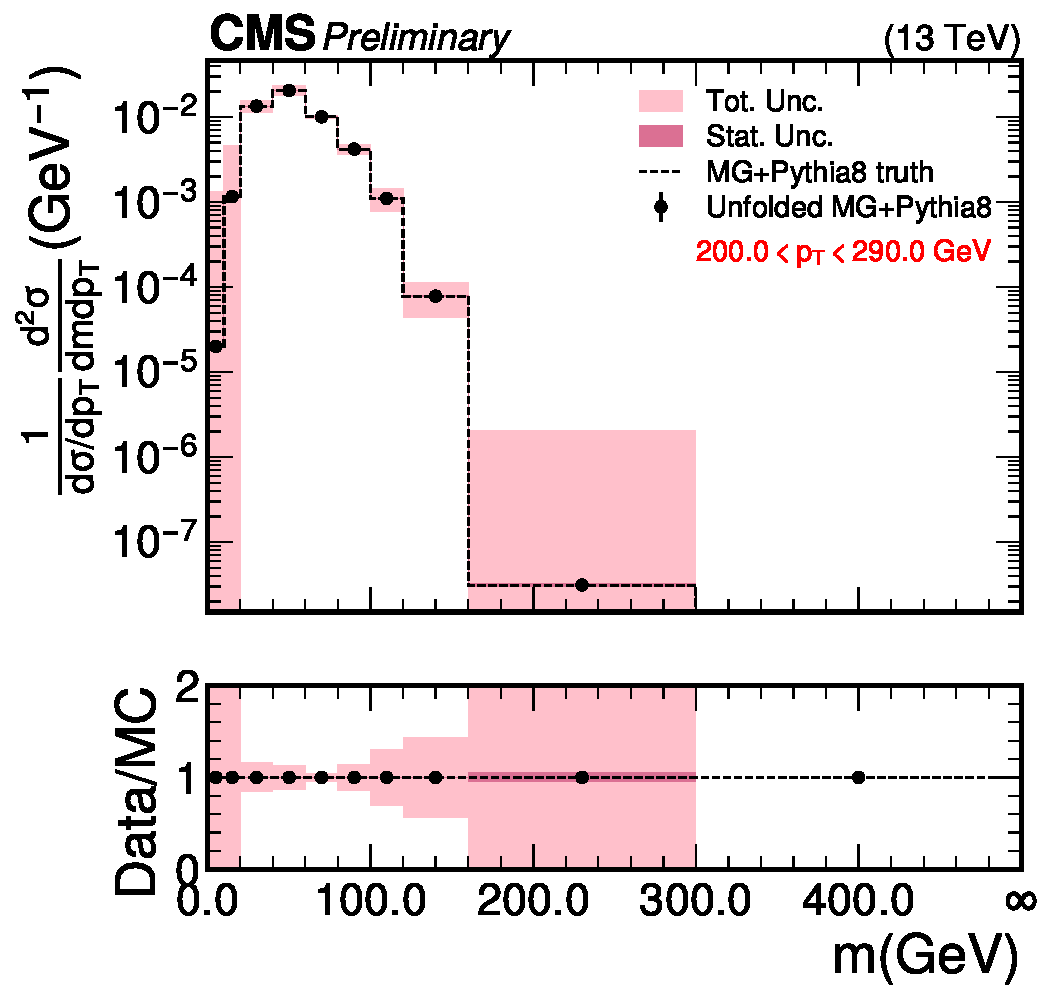
\includegraphics[width=0.45\textwidth]{figures/multijet/unfolding/trijet/closure_binnedResult_ungroomed_0.pdf}
        \end{subfigure}%
        \begin{subfigure}
          \centering
          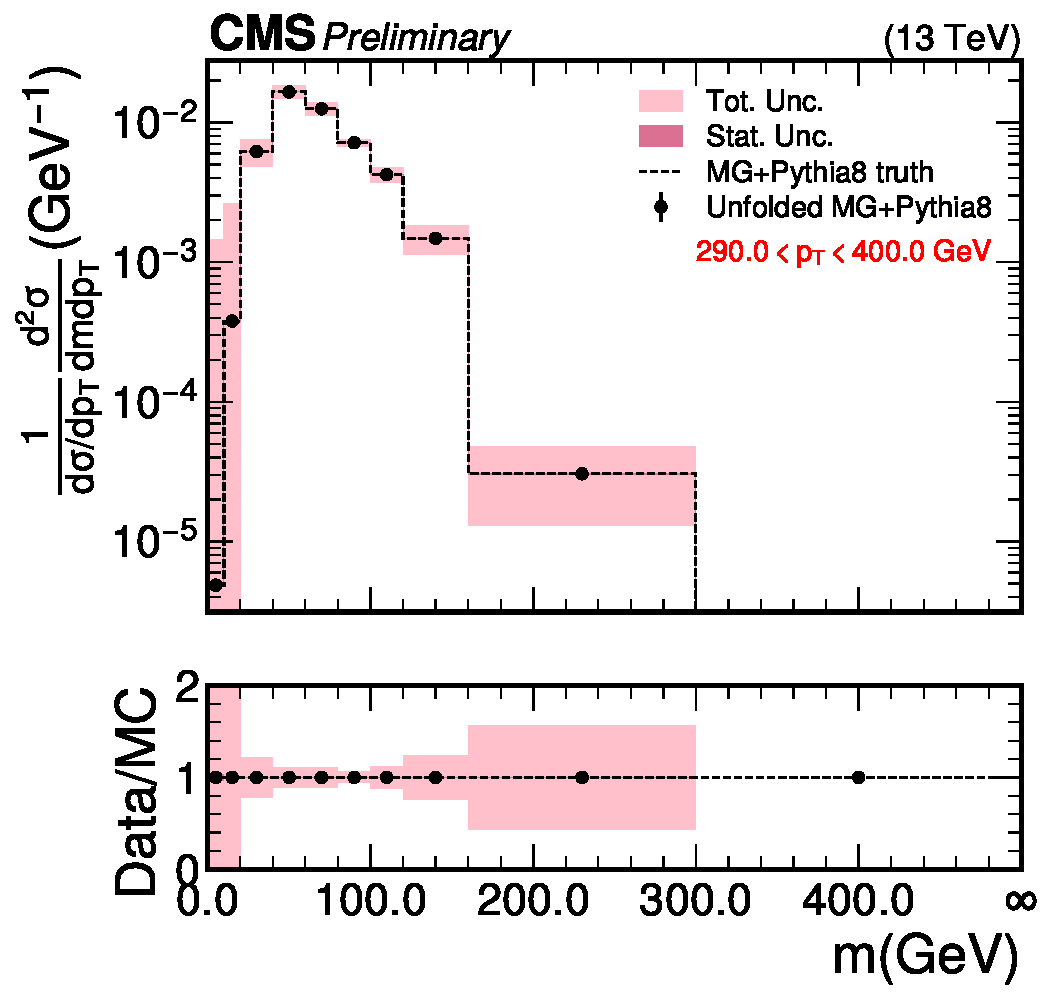
\includegraphics[width=0.45\textwidth]{figures/multijet/unfolding/trijet/closure_binnedResult_ungroomed_1.pdf}
        \end{subfigure}%
        \begin{subfigure}
          \centering
          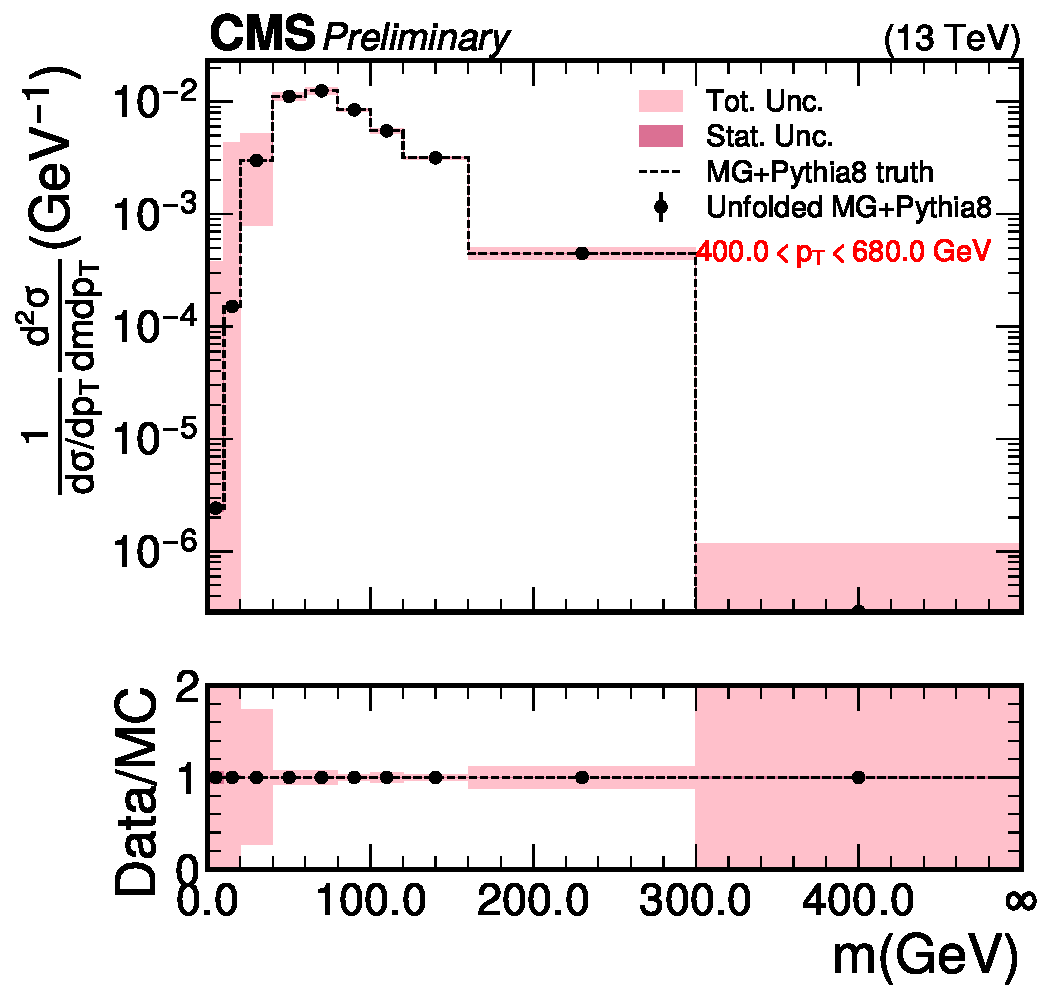
\includegraphics[width=0.45\textwidth]{figures/multijet/unfolding/trijet/closure_binnedResult_ungroomed_2.pdf}
        \end{subfigure}%
        \begin{subfigure}
          \centering
          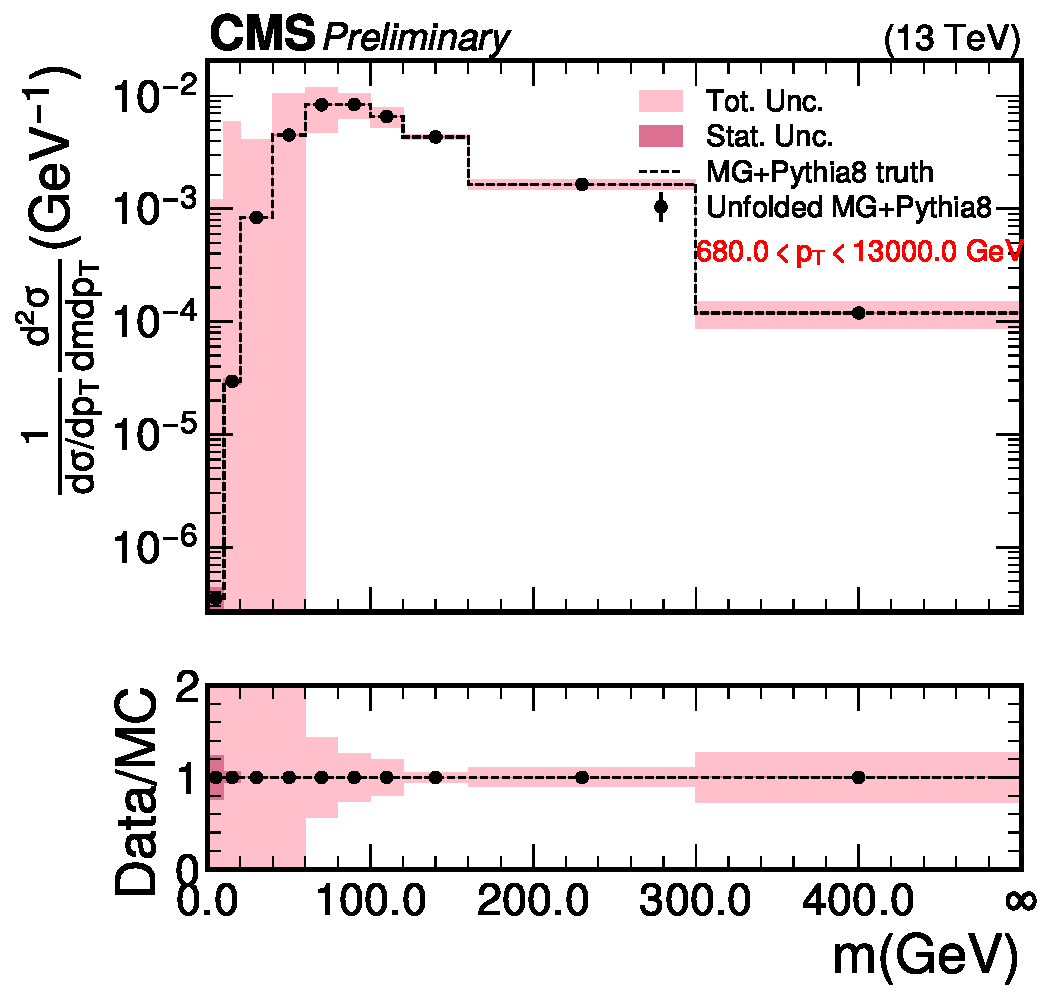
\includegraphics[width=0.45\textwidth]{figures/multijet/unfolding/trijet/closure_binnedResult_ungroomed_3.pdf}
        \end{subfigure}
        \caption{Trijet self-closure test results for the ungroomed jet mass.}
	\label{fig:trijetclosurebinned_u}
      \end{figure}

      \begin{figure}[htp!]
        \begin{subfigure}
          \centering
          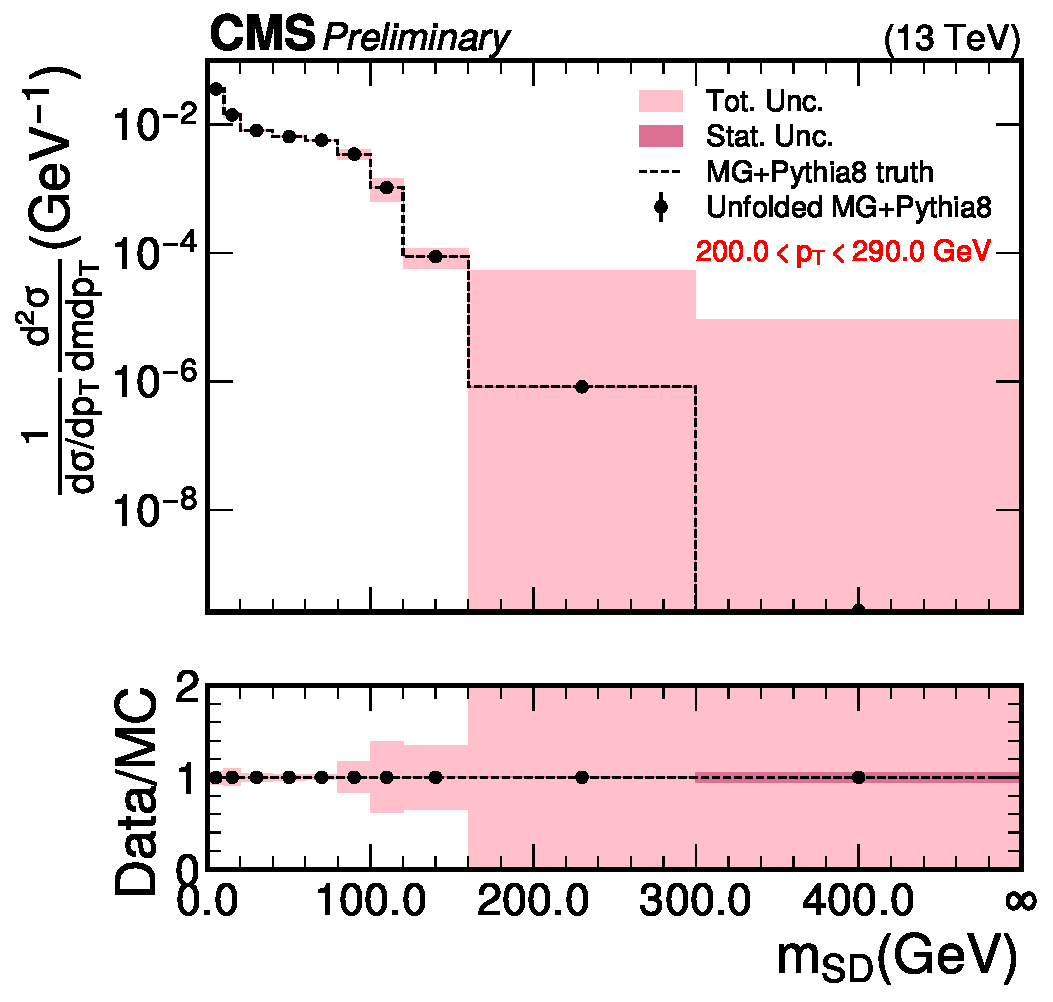
\includegraphics[width=0.45\textwidth]{figures/multijet/unfolding/trijet/closure_binnedResult_groomed_0.pdf}
        \end{subfigure} 
        \begin{subfigure}
          \centering
          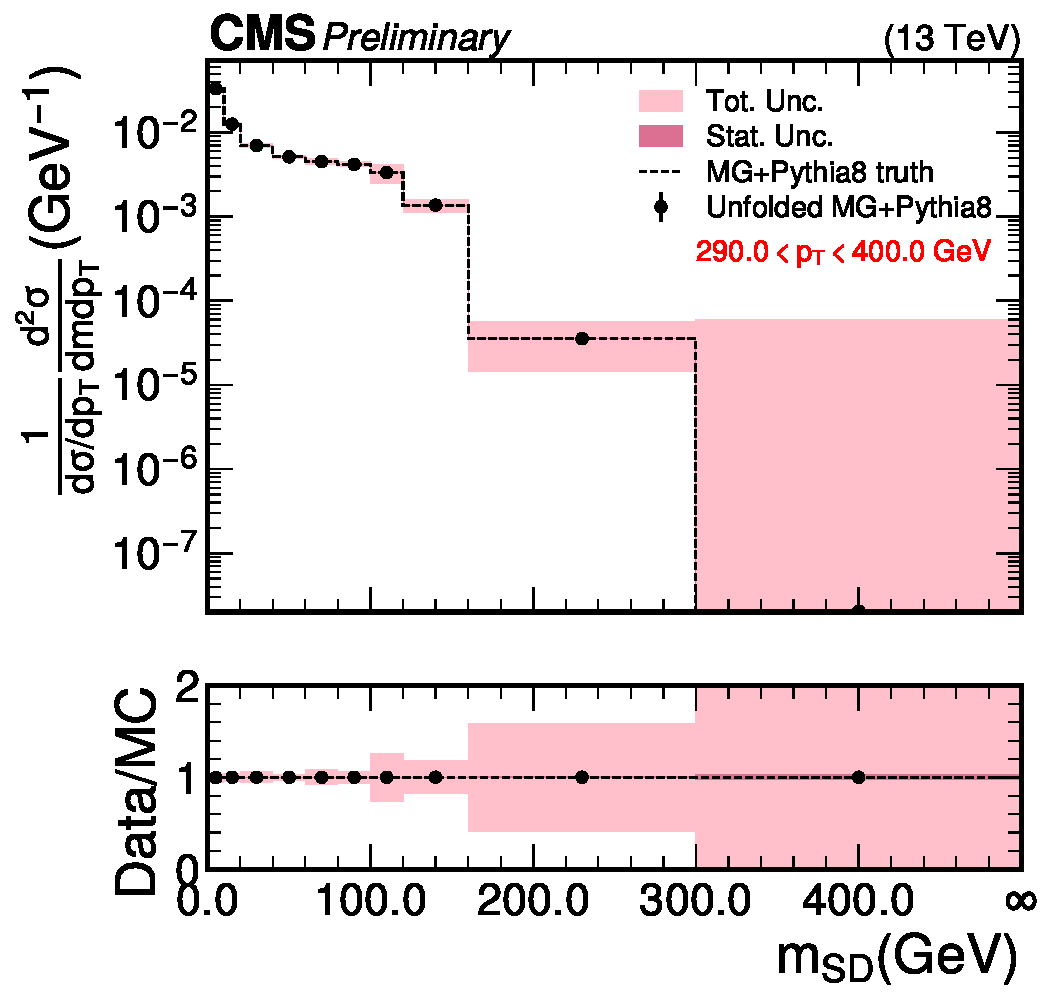
\includegraphics[width=0.45\textwidth]{figures/multijet/unfolding/trijet/closure_binnedResult_groomed_1.pdf}
        \end{subfigure}
        \begin{subfigure}
          \centering
          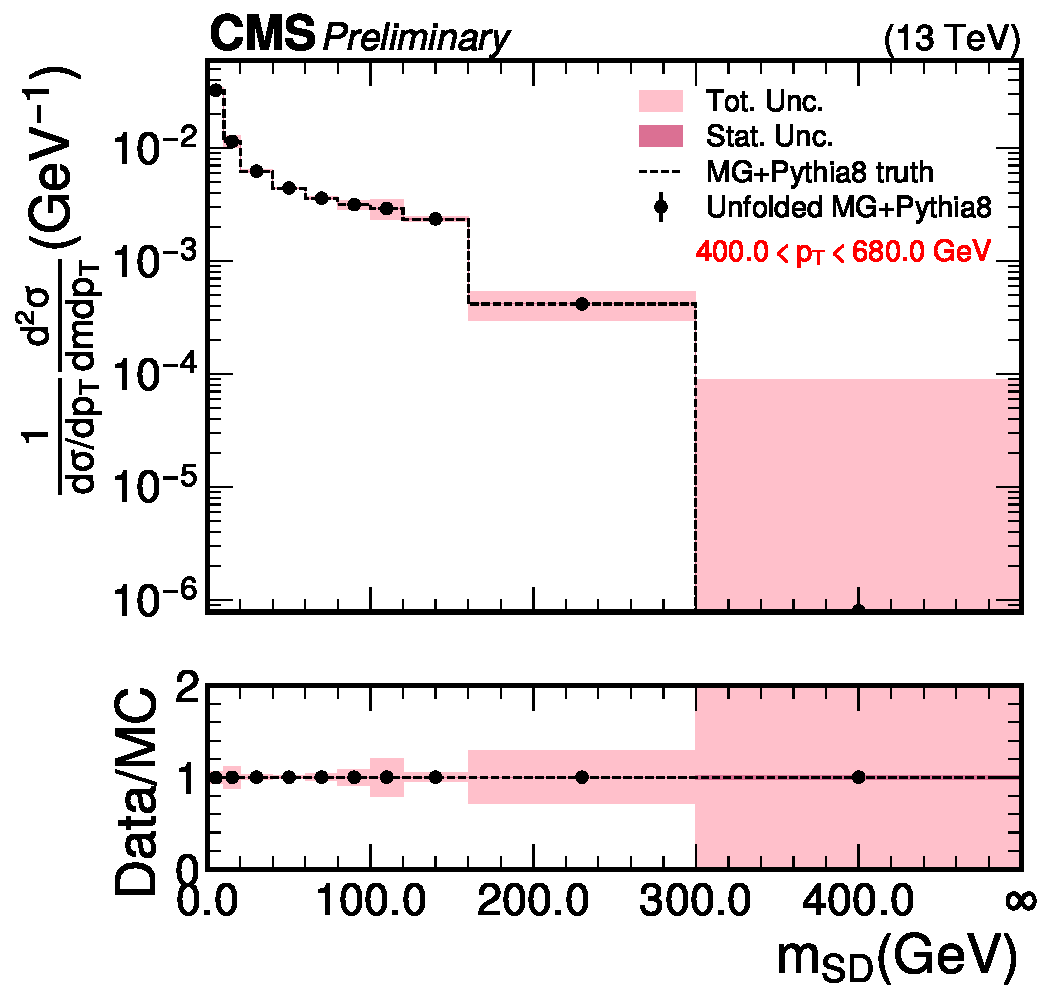
\includegraphics[width=0.45\textwidth]{figures/multijet/unfolding/trijet/closure_binnedResult_groomed_2.pdf}
        \end{subfigure} 
        \begin{subfigure}
          \centering
          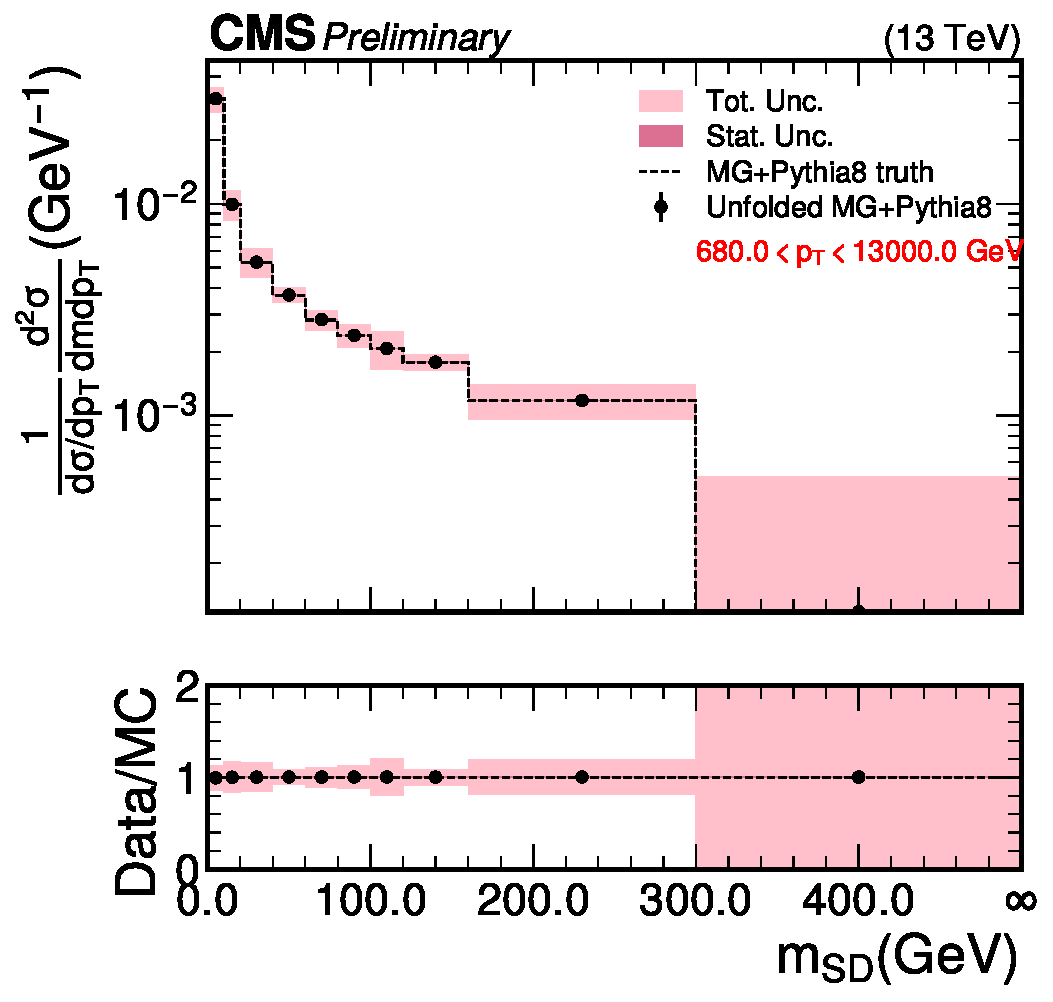
\includegraphics[width=0.45\textwidth]{figures/multijet/unfolding/trijet/closure_binnedResult_groomed_3.pdf}
        \end{subfigure} \\
	\caption{Trijet self-closure test results for the groomed jet mass.}
	\label{fig:trijetclosurebinned_g}
      \end{figure}
 \begin{figure}[htp!]
	\centering
	\begin{subfigure}
          \centering
          \includegraphics[width=0.45\textwidth]{figures/multijet/unfolding/dijet/closure_herwig_binnedResult_ungroomed_0.pdf}
        \end{subfigure}%
        \begin{subfigure}
          \centering
          \includegraphics[width=0.45\textwidth]{figures/multijet/unfolding/dijet/closure_herwig_binnedResult_ungroomed_1.pdf}
        \end{subfigure}%
        \begin{subfigure}
          \centering
          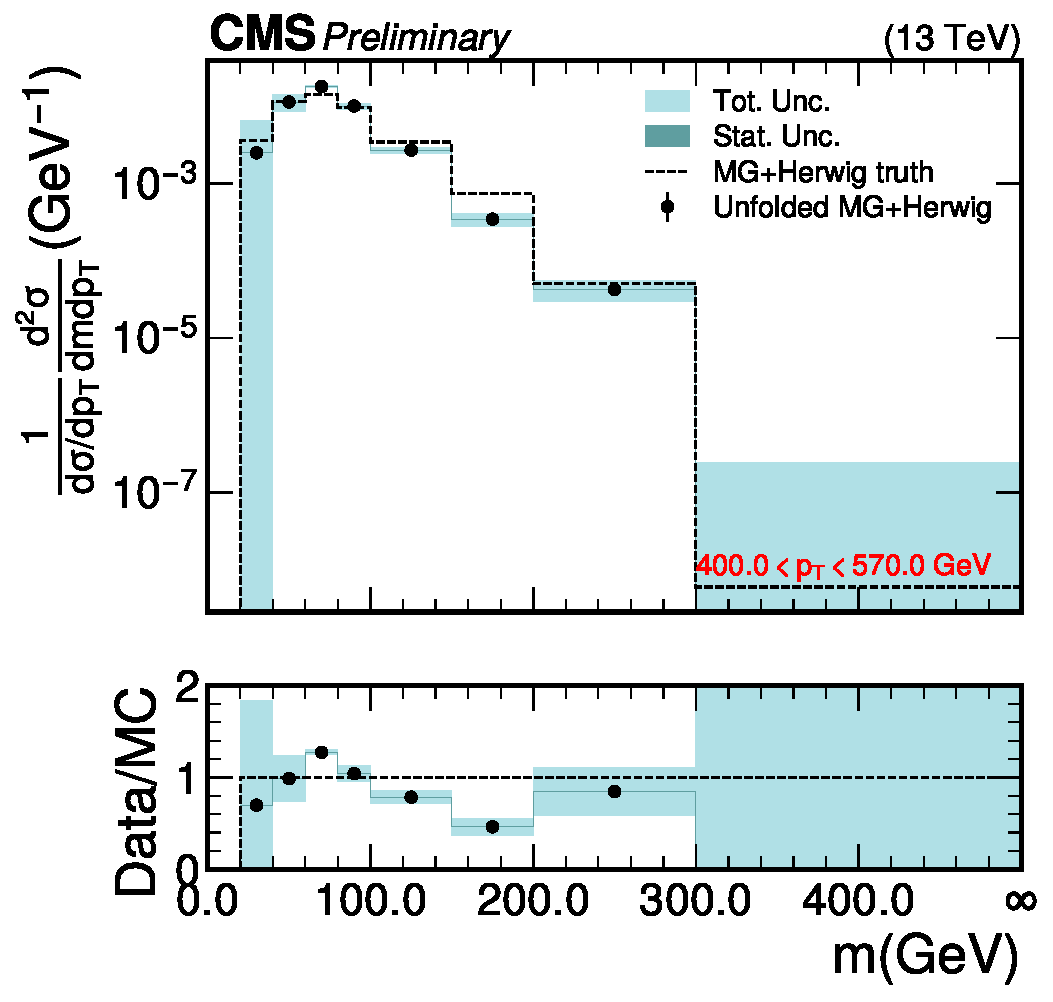
\includegraphics[width=0.45\textwidth]{figures/multijet/unfolding/dijet/closure_herwig_binnedResult_ungroomed_2.pdf}
        \end{subfigure}%
        \begin{subfigure}
          \centering
          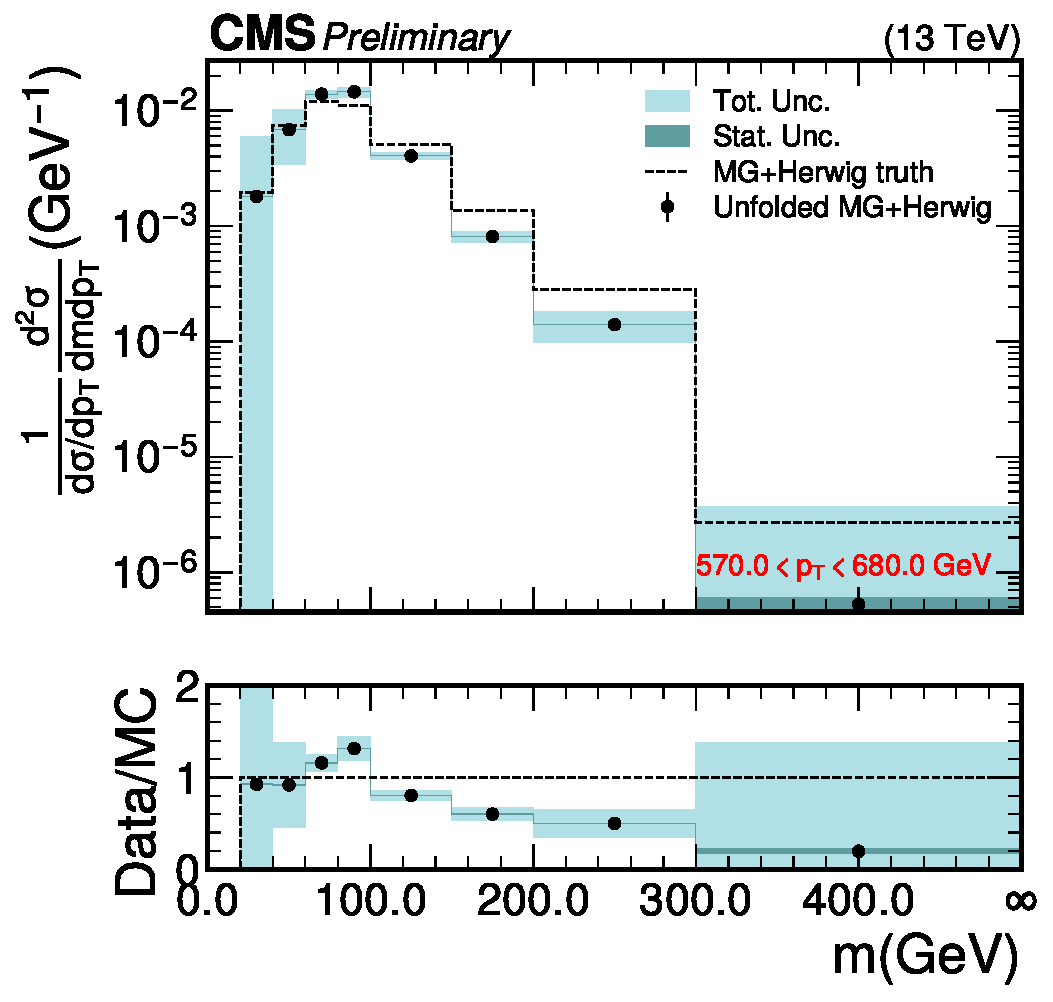
\includegraphics[width=0.45\textwidth]{figures/multijet/unfolding/dijet/closure_herwig_binnedResult_ungroomed_3.pdf}
        \end{subfigure}
        \begin{subfigure}
          \centering
          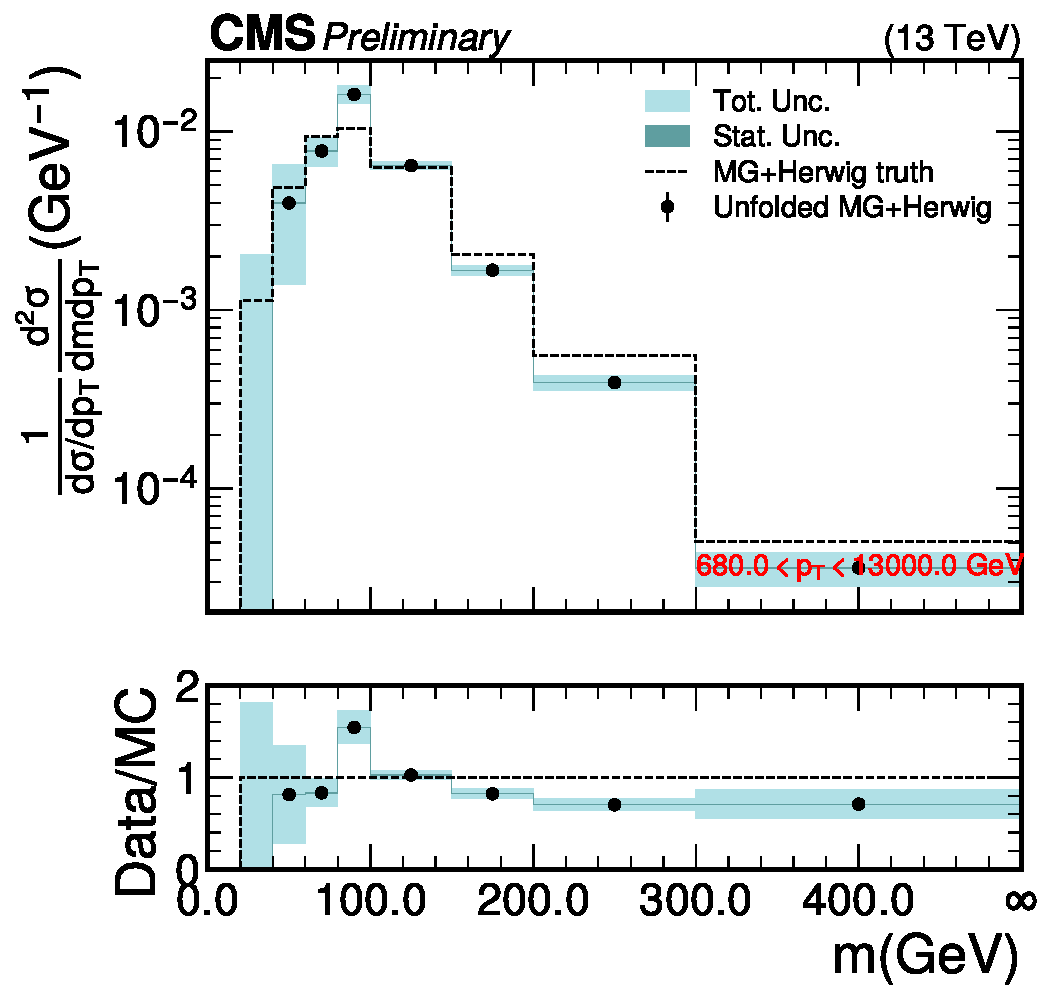
\includegraphics[width=0.45\textwidth]{figures/multijet/unfolding/dijet/closure_herwig_binnedResult_ungroomed_4.pdf}
        \end{subfigure}
        \caption{Dijet MG+HERWIG samples unfolded with the MG+Pythia8 response matrix compared to MG+HERWIG truth for the ungroomed jet mass.}
	\label{fig:dijetherwigclosurebinned_u}
      \end{figure}

      \begin{figure}[htp!]
        \begin{subfigure}
          \centering
          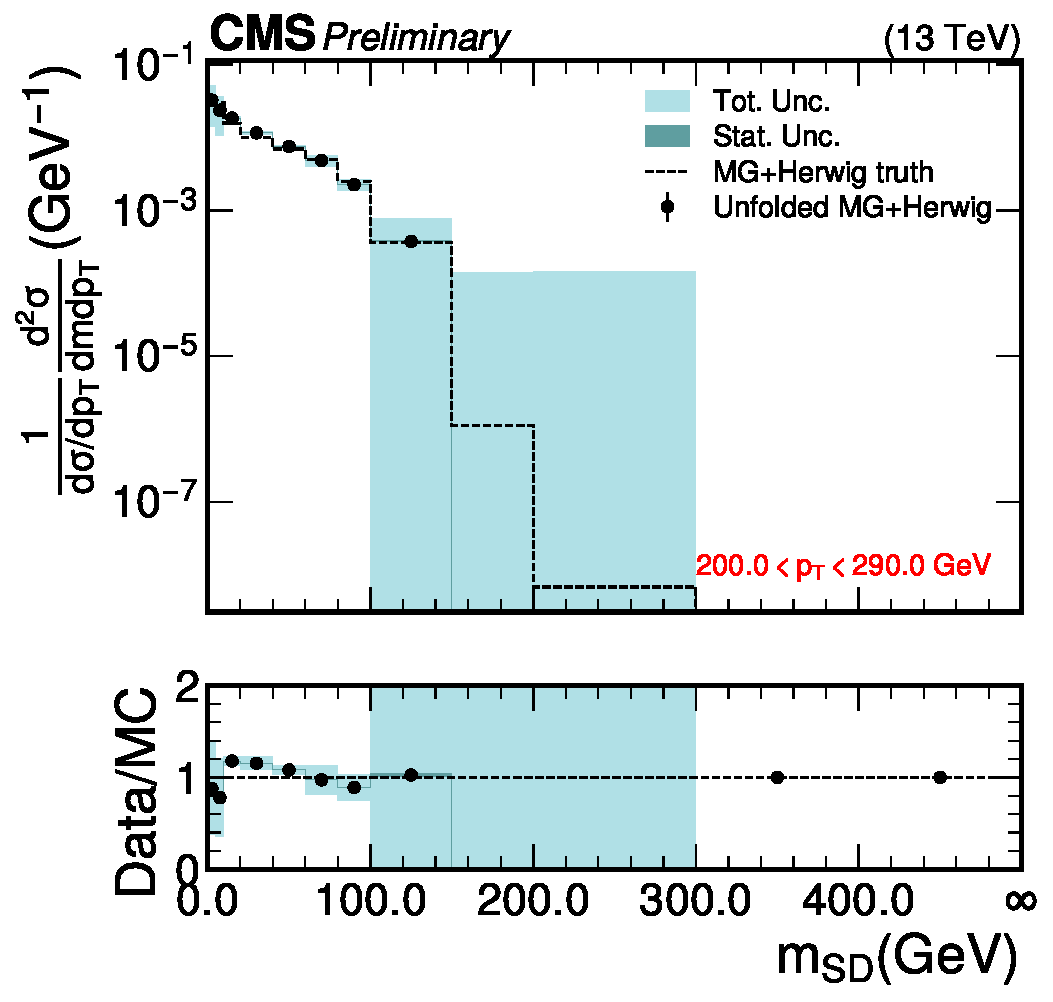
\includegraphics[width=0.45\textwidth]{figures/multijet/unfolding/dijet/closure_herwig_binnedResult_groomed_0.pdf}
        \end{subfigure} 
        \begin{subfigure}
          \centering
          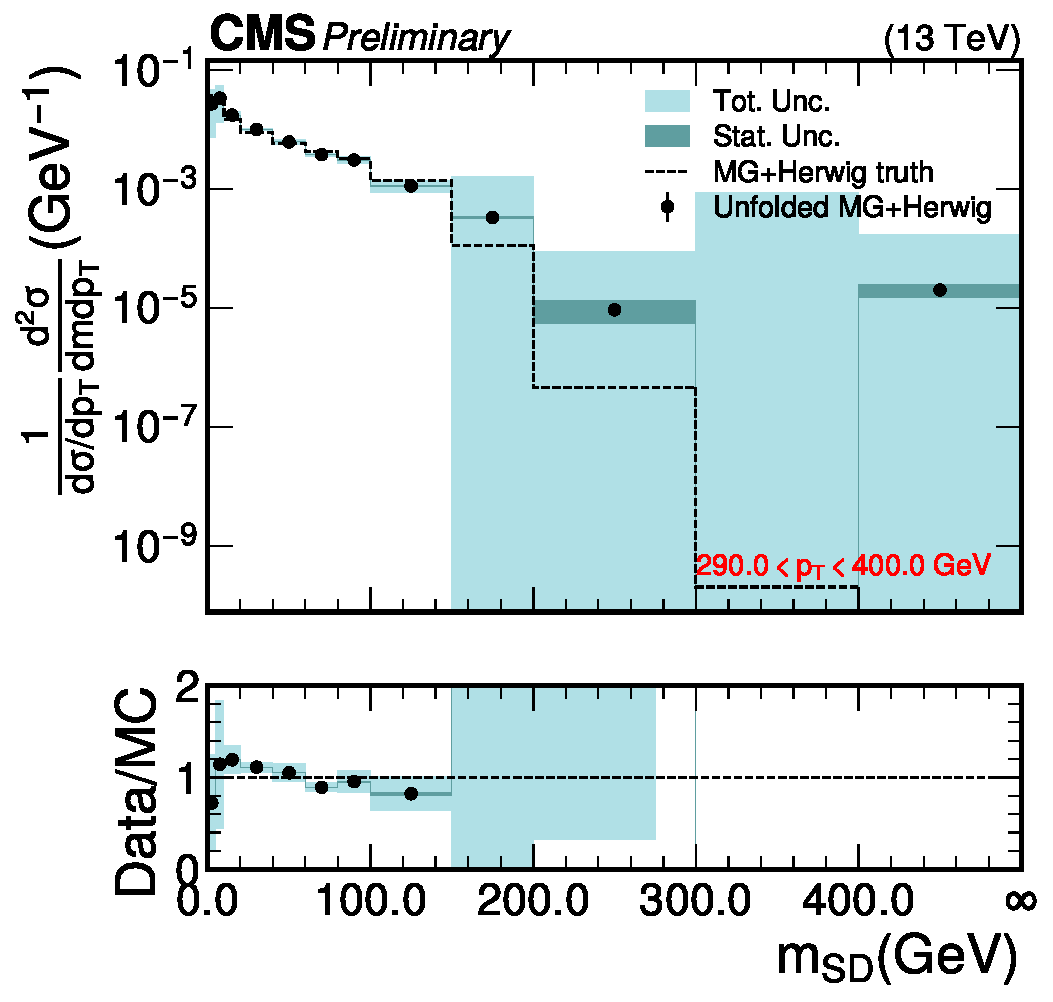
\includegraphics[width=0.45\textwidth]{figures/multijet/unfolding/dijet/closure_herwig_binnedResult_groomed_1.pdf}
        \end{subfigure}
        \begin{subfigure}
          \centering
          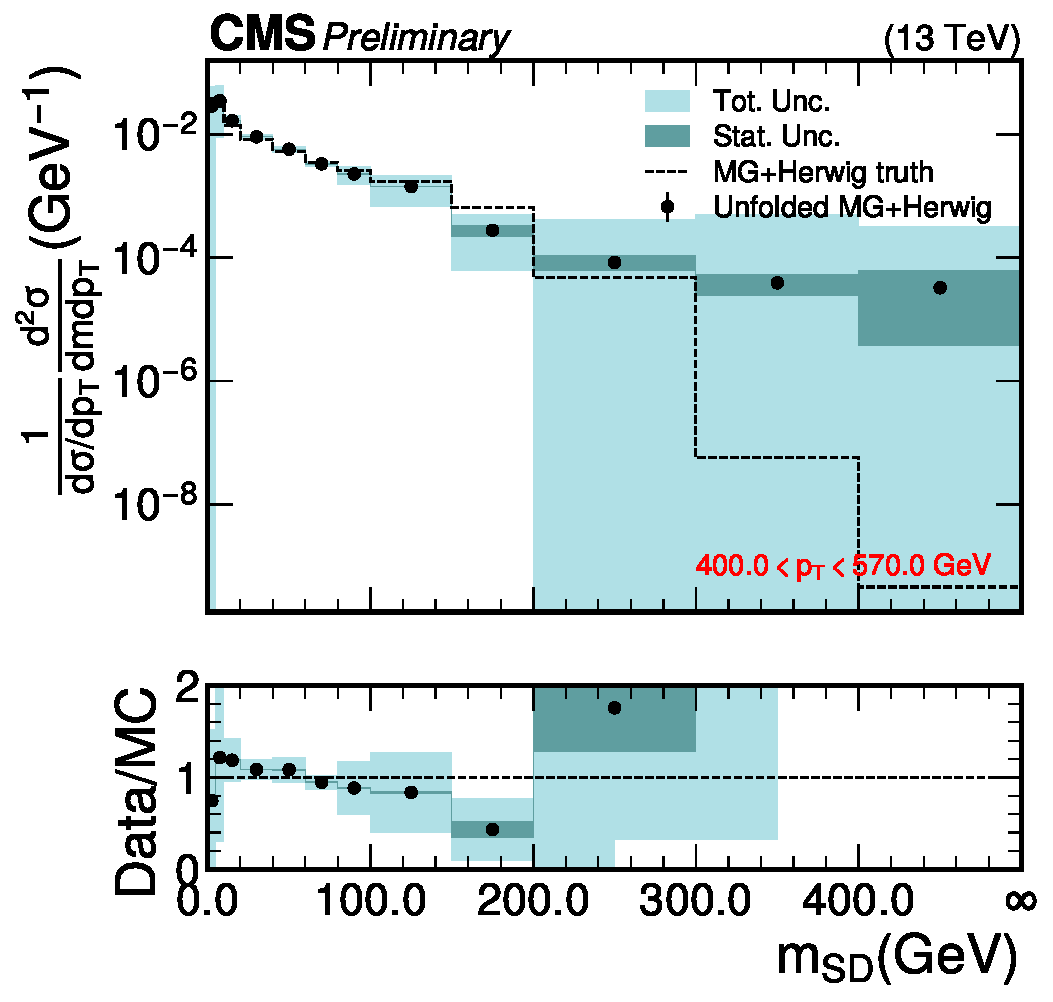
\includegraphics[width=0.45\textwidth]{figures/multijet/unfolding/dijet/closure_herwig_binnedResult_groomed_2.pdf}
        \end{subfigure} 
        \begin{subfigure}
          \centering
          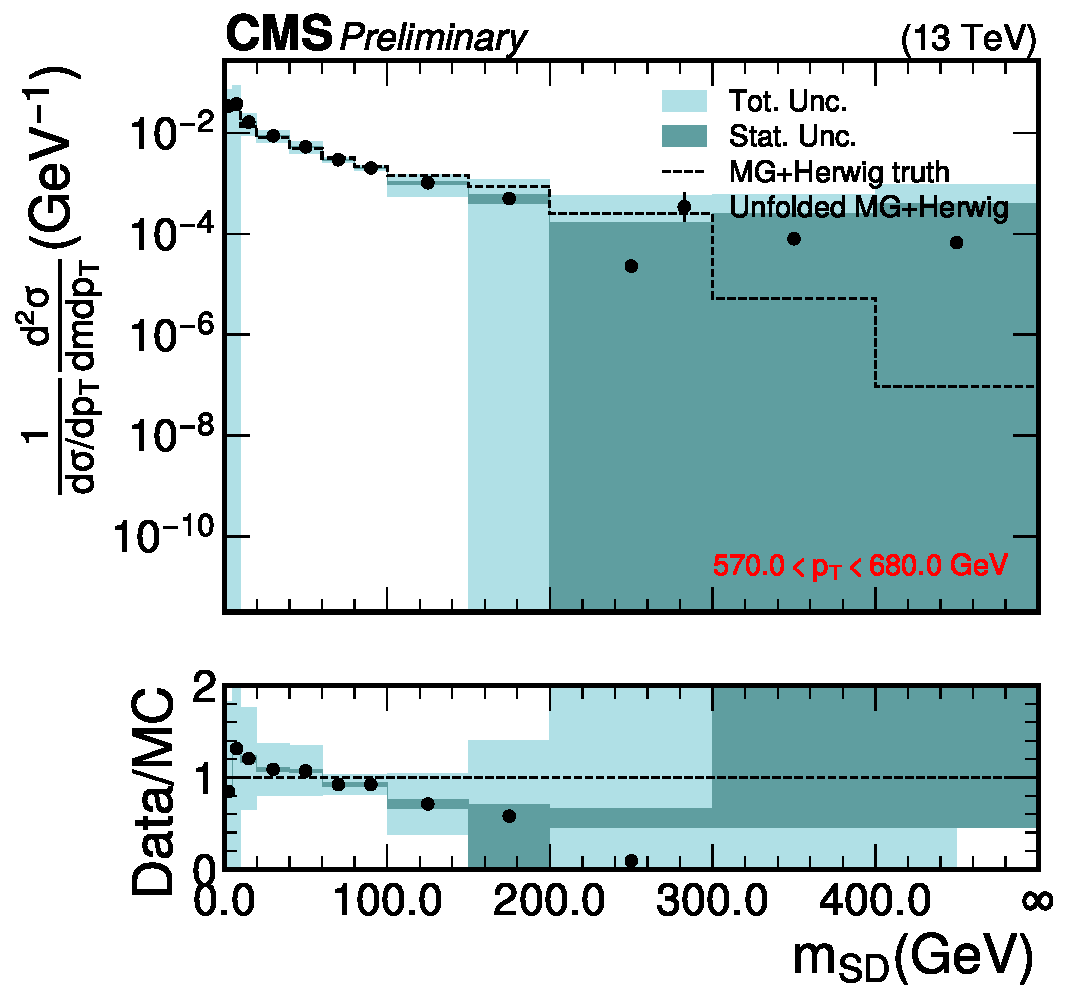
\includegraphics[width=0.45\textwidth]{figures/multijet/unfolding/dijet/closure_herwig_binnedResult_groomed_3.pdf}
        \end{subfigure}
        \begin{subfigure}
          \centering
          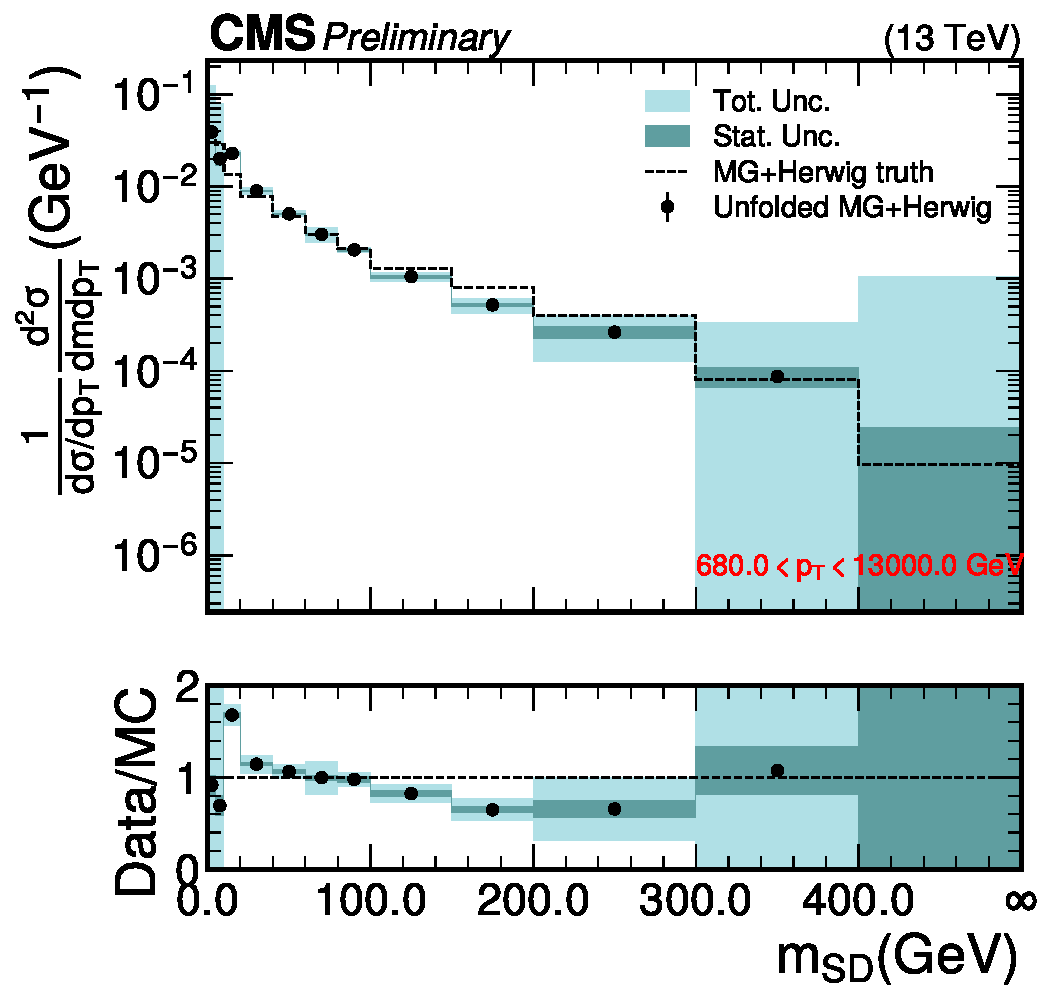
\includegraphics[width=0.45\textwidth]{figures/multijet/unfolding/dijet/closure_herwig_binnedResult_groomed_4.pdf}
        \end{subfigure}\\
	\caption{Dijet MG+HERWIG samples unfolded with the MG+Pythia8 response matrix compared to MG+HERWIG truth for the groomed jet mass.}
	\label{fig:dijetherwigclosurebinned_g}
      \end{figure}
      
      \begin{figure}[htp!]
	\centering
	\begin{subfigure}
          \centering
          \includegraphics[width=0.45\textwidth]{figures/multijet/unfolding/trijet/closure_herwig_binnedResult_ungroomed_0.pdf}
        \end{subfigure}%
        \begin{subfigure}
          \centering
          \includegraphics[width=0.45\textwidth]{figures/multijet/unfolding/trijet/closure_herwig_binnedResult_ungroomed_1.pdf}
        \end{subfigure}%
        \begin{subfigure}
          \centering
          \includegraphics[width=0.45\textwidth]{figures/multijet/unfolding/trijet/closure_herwig_binnedResult_ungroomed_2.pdf}
        \end{subfigure}%
        \begin{subfigure}
          \centering
          \includegraphics[width=0.45\textwidth]{figures/multijet/unfolding/trijet/closure_herwig_binnedResult_ungroomed_3.pdf}
        \end{subfigure}
        \caption{Trijet MG+HERWIG samples unfolded with the MG+Pythia8 response matrix compared to MG+HERWIG truth for the ungroomed jet mass.}
	\label{fig:trijetherwigclosurebinned_u}
      \end{figure}

      \begin{figure}[htp!]
        \begin{subfigure}
          \centering
          \includegraphics[width=0.45\textwidth]{figures/multijet/unfolding/trijet/closure_herwig_binnedResult_groomed_0.pdf}
        \end{subfigure} 
        \begin{subfigure}
          \centering
          \includegraphics[width=0.45\textwidth]{figures/multijet/unfolding/trijet/closure_herwig_binnedResult_groomed_1.pdf}
        \end{subfigure}
        \begin{subfigure}
          \centering
          \includegraphics[width=0.45\textwidth]{figures/multijet/unfolding/trijet/closure_herwig_binnedResult_groomed_2.pdf}
        \end{subfigure} 
        \begin{subfigure}
          \centering
          \includegraphics[width=0.45\textwidth]{figures/multijet/unfolding/trijet/closure_herwig_binnedResult_groomed_3.pdf}
        \end{subfigure} \\
	\caption{Trijet MG+HERWIG samples unfolded with the MG+Pythia8 response matrix compared to MG+HERWIG truth for the ungroomed jet mass.}
	\label{fig:trijetherwigclosurebinned_g}
      \end{figure}

      \subsection{Bottom line test}
      
      Aa a sanity check that the unfolding does not introduce additional discrepancies between data and simulation, the ratio of the unfolded result and the truth are compared to the data. Ideally the unfolded result will not bring the distribution further from agreement with data compared to the MC truth. These bottom line test plots can be seen in Figures \ref{fig:dijet_bottomline} and \ref{fig:trijet_bottomline} and it can be seen that the unfolded results are fairly stable across the bins and have better agreement in the groomed channel.
        \begin{figure}[htp!]
        \begin{subfigure}
          \centering
          \includegraphics[width=0.45\textwidth]{figures/multijet/unfolding/dijet/biastest_u.pdf}
        \end{subfigure} 
        \begin{subfigure}
          \centering
          \includegraphics[width=0.45\textwidth]{figures/multijet/unfolding/dijet/biastest_g.pdf}
        \end{subfigure} \\
	\caption{Dijet bottom line tests for the ungroomed mass (left column) and groomed mass (right column).}
	\label{fig:dijet_bottomline}
      \end{figure}
            \begin{figure}[htp!]
        \begin{subfigure}
          \centering
          \includegraphics[width=0.45\textwidth]{figures/multijet/unfolding/trijet/biastest_u.pdf}
        \end{subfigure} 
        \begin{subfigure}
          \centering
          \includegraphics[width=0.45\textwidth]{figures/multijet/unfolding/trijet/biastest_g.pdf}
        \end{subfigure} \\
	\caption{Dijet bottom line tests for the ungroomed mass (left column) and groomed mass (right column).}
	\label{fig:trijet_bottomline}
      \end{figure}
       \section{Results and summary}
  Normalized, double differential cross-section measurements with respect to jet mass and \pt of the dijet and softest jet of trijet events are presented here, using proton-proton collision data taken at a center of mass energy of$ \sqrt{s} = 13$ TeV from the combined years 2016, 2017, and 2018, corresponding to an integrated luminosity of $137.6 fb^{-1}$. The cross-sections with respect to soft drop groomed mass and ungroomed mass were measured separately for boosted jets with a radius parameter of $R=0.8$. The goal of this measurement is to provide verification of jet mass modelling for quark and gluon jets by looking at the resulting cross-sections with respect to mass for channels of varying quark and gluon content and with and without softdrop grooming applied to get a handle on the modelling of the soft content of these jets. The dijet channel is a quark-gluon admixture, and the results for the normalized differential cross section with respect to the ungroomed mass are shown in Fig. \ref{fig:dijetresultsbinned_u}, and with respect to the groomed mass in Fig. \ref{fig:dijetresultsbinned_g}. Bins with \jetmass $<20 GeV$ and where the total uncertainty is $> 60\%$ have been removed. We see that there is agreement between the unfolded data and simulation for all bins except the highest mass bin in the highest \pt bin where the simulation breaks down. The trijet channel shows the softest jet of three QCD jets and is gluon enriched, the results for the ungroomed mass can be seen in Fig.  \ref{fig:trijetresultsbinned_u} and for the groomed case in Fig. \ref{fig:trijetresultsbinned_g}. Again, bins with \jetmass $<20 GeV$ and where the total uncertainty is $> 60\%$ have been removed. For the trijet case there are much lower statistics, but we still observe fairly good agreement between the unfolded data and simulation.
  \begin{figure}[htp!]
    \centering
    \begin{subfigure}
      \centering
      \includegraphics[width=0.45\textwidth]{figures/multijet/unfolding/dijet/binnedResult_ungroomed_0.pdf}
    \end{subfigure}%
    \begin{subfigure}
      \centering
      \includegraphics[width=0.45\textwidth]{figures/multijet/unfolding/dijet/binnedResult_ungroomed_1.pdf}
    \end{subfigure}%
    \begin{subfigure}
      \centering
      \includegraphics[width=0.45\textwidth]{figures/multijet/unfolding/dijet/binnedResult_ungroomed_2.pdf}
    \end{subfigure}%
    \begin{subfigure}
      \centering
      \includegraphics[width=0.45\textwidth]{figures/multijet/unfolding/dijet/binnedResult_ungroomed_3.pdf}
    \end{subfigure}
    \begin{subfigure}
      \centering
      \includegraphics[width=0.45\textwidth]{figures/multijet/unfolding/dijet/binnedResult_ungroomed_4.pdf}
    \end{subfigure}
    \caption{Unfolded, normalized differential cross-sections with respect to \textbf{ungroomed} jet mass and \pt for the \textbf{dijet} channel. }
    \label{fig:dijetresultsbinned_u}
  \end{figure}
  
  \begin{figure}[htp!]
    \begin{subfigure}
      \centering
      \includegraphics[width=0.45\textwidth]{figures/multijet/unfolding/dijet/binnedResult_groomed_0.pdf}
    \end{subfigure} 
    \begin{subfigure}
      \centering
      \includegraphics[width=0.45\textwidth]{figures/multijet/unfolding/dijet/binnedResult_groomed_1.pdf}
    \end{subfigure}
    \begin{subfigure}
      \centering
      \includegraphics[width=0.45\textwidth]{figures/multijet/unfolding/dijet/binnedResult_groomed_2.pdf}
    \end{subfigure} 
    \begin{subfigure}
      \centering
      \includegraphics[width=0.45\textwidth]{figures/multijet/unfolding/dijet/binnedResult_groomed_3.pdf}
    \end{subfigure}
    \begin{subfigure}
      \centering
      \includegraphics[width=0.45\textwidth]{figures/multijet/unfolding/dijet/binnedResult_groomed_4.pdf}
    \end{subfigure}\\
    \caption{Unfolded, normalized differential cross-sections with respect to \textbf{soft drop groomed} mass and \pt for the \textbf{dijet} channel.}
    \label{fig:dijetresultsbinned_g}
  \end{figure}
  
  \begin{figure}[htp!]
    \centering
    \begin{subfigure}
      \centering
      \includegraphics[width=0.45\textwidth]{figures/multijet/unfolding/trijet/binnedResult_ungroomed_0.pdf}
    \end{subfigure}%
    \begin{subfigure}
      \centering
      \includegraphics[width=0.45\textwidth]{figures/multijet/unfolding/trijet/binnedResult_ungroomed_1.pdf}
    \end{subfigure}%
    \begin{subfigure}
      \centering
      \includegraphics[width=0.45\textwidth]{figures/multijet/unfolding/trijet/binnedResult_ungroomed_2.pdf}
    \end{subfigure}%
    \begin{subfigure}
      \centering
      \includegraphics[width=0.45\textwidth]{figures/multijet/unfolding/trijet/binnedResult_ungroomed_3.pdf}
    \end{subfigure}
    \caption{Unfolded, normalized differential cross-sections with respect to \textbf{ungroomed} mass and \pt for the \textbf{trijet} channel.}
    \label{fig:trijetresultsbinned_u}
  \end{figure}
  
  \begin{figure}[htp!]
    \begin{subfigure}
      \centering
      \includegraphics[width=0.45\textwidth]{figures/multijet/unfolding/trijet/binnedResult_groomed_0.pdf}
    \end{subfigure} 
    \begin{subfigure}
      \centering
      \includegraphics[width=0.45\textwidth]{figures/multijet/unfolding/trijet/binnedResult_groomed_1.pdf}
    \end{subfigure}
    \begin{subfigure}
      \centering
      \includegraphics[width=0.45\textwidth]{figures/multijet/unfolding/trijet/binnedResult_groomed_2.pdf}
    \end{subfigure} 
    \begin{subfigure}
      \centering
      \includegraphics[width=0.45\textwidth]{figures/multijet/unfolding/trijet/binnedResult_groomed_3.pdf}
    \end{subfigure} \\
    \caption{Unfolded, normalized differential cross-sections with respect to \textbf{softdrop groomed} mass and \pt for the \texbf{trijet} channel.}
    \label{fig:trijetresultsbinned_g}
  \end{figure}
  \newpage



